\appendix
\clearpage
\setcounter{figure}{0}
\setcounter{table}{0}
\setcounter{page}{1}
\onecolumn


% \setlength{\oddsidemargin}{1.875in}
% \setlength{\evensidemargin}{1.875in}
% \addtolength{\textwidth}{-3.75in}

\newlength\addedmarginsingle
\setlength\addedmarginsingle{0.875in}
\newlength\addedmargintotal
\setlength\addedmargintotal{2\addedmarginsingle}

\addtolength{\oddsidemargin}{\addedmarginsingle}
\addtolength{\evensidemargin}{\addedmarginsingle}
\addtolength{\textwidth}{-\addedmargintotal}
\addtolength{\linewidth}{-\addedmargintotal}
\addtolength{\hsize}{-\addedmargintotal}
\addtolength{\topmargin}{\addedmarginsingle}
\addtolength{\textheight}{-\addedmargintotal}
\addtolength{\vsize}{-\addedmargintotal}

\pagestyle{plain}

\clearpage
% \thispagestyle{empty}\ \

\thispagestyle{empty}
\ \\ \ \\ \ \\ \ \\ \ \\
\begin{center}
 {\Huge Bringing biological networks}\\ \ \\ {\Huge to life with ANIMO}\\ \ \\ \ \\
 {\huge Additional Materials}
\end{center}
\clearpage






\makeatletter

% Copied from the LaTeX sources
\def\addcontentsline#1#2#3{%
  \addtocontents{#1}{\protect\contentsline{#2}{#3}{\thepage}}}
\long\def\addtocontents#1#2{%
  \protected@write\@auxout
    {\let\label\@gobble \let\index\@gobble \let\glossary\@gobble}%
    {\string\@writefile{#1}{#2}}}
\titlecontents{section} % set formatting for \section -
                        % \subsection must be formatted separately
[2.em]                 % adjust left margin
{\bf}             % font formatting
{\contentslabel{2.em}} % section label and offset
{\hspace*{-2.em}}
{\titlerule*[1pc]{}\contentspage}
\titlecontents{subsection} % set formatting for \section -
                        % \subsection must be formatted separately
[4.5em]                 % adjust left margin
{\rmfamily}             % font formatting
{\contentslabel{2.5em}} % section label and offset
{\hspace*{2.5em}}
{\titlerule*[1pc]{.}\contentspage}
% Copied from article.cls
%\setcounter{tocdepth}{5}
\newcommand\tableofcontents{%
\begin{spacing}{1.3}
    \section*{\contentsname
        \@mkboth{%
           \MakeUppercase\contentsname}{\MakeUppercase\contentsname}}%
    \@starttoc{toc}%
\end{spacing}
}
% \newcommand*\l@paragraph{\@dottedtocline{4}{7.0em}{4.1em}}
% \newcommand*\l@subparagraph{\@dottedtocline{5}{10em}{5em}}
% \newcommand\listoffigures{%
%     \section*{\listfigurename}%
%       \@mkboth{\MakeUppercase\listfigurename}%
%               {\MakeUppercase\listfigurename}%
%     \@starttoc{lof}%
%     }
% \newcommand*\l@figure{\@dottedtocline{1}{1.5em}{2.3em}}
% \newcommand\listoftables{%
%     \section*{\listtablename}%
%       \@mkboth{%
%           \MakeUppercase\listtablename}%
%          {\MakeUppercase\listtablename}%
%     \@starttoc{lot}%
%     }
% \let\l@table\l@figure

\makeatother




\addtocontents{toc}{\protect\setcounter{tocdepth}{5}}
\thispagestyle{empty}
\tableofcontents
\clearpage

\setcounter{page}{1}
\setcounter{section}{0}

\renewcommand\figurename{Figure}
\renewcommand*\thefigure{S\arabic{figure}}
\renewcommand*\thetable{S\arabic{table}}

\def\ta{TA}
\def\tas{TA}




\section{Requirements and installation}\label{sec:animo-installation}
In order to run ANIMO, a desktop or laptop computer is needed with the following software installed:
\begin{itemize}
  \item Java: see Section~\ref{sec:install-java}
  \item Cytoscape~\citep{cytoscape}: see Section~\ref{sec:install-cytoscape}
  \item UPPAAL~\citep{uppaal}: see Section~\ref{sec:install-uppaal}
\end{itemize}
Each works under Windows~(\winsymbol), Mac-OS~(\macsymbol) and all most common GNU/Linux~(\linuxsymbol) distributions.
If the requirements are already met, ANIMO can be directly installed following the instructions in Section~\ref{sec:install-animo}.\\
\emph{Note}: when required to type something, the text to input will be represented ``{\tt like this}'': the quotation marks
are not intended to be typed.

\subsection{Java}\label{sec:install-java}
\begin{enumerate}
\item\label{step:open-console} In order to check that Java is installed, open a console
\winmaclinux{Windows 7: press Windows button and type ``{\tt cmd}'', then press Return. Previous versions: in the Start
menu find \emph{All programs} $\rightarrow$ \emph{Accessories} $\rightarrow$ \emph{Command Prompt}.}%
{Go to \emph{Applications} $\rightarrow$ \emph{Utilities} $\rightarrow$ \emph{Terminal}.}%
{Under Gnome, press Alt-F2, type ``{\tt gnome-terminal}'', then press Return. Under KDE, press the KMenu button, type
``{\tt konsole}'' and click Konsole. Under Unity, press the home button (the one with the Ubuntu
logo:~\ubuntusymbol), type ``{\tt terminal}'' and click the Terminal icon.}
\item Type ``{\tt java}'' and press Return. If a brief error message like ``{\tt unknown command}'' is shown, Java needs to be
installed: please proceed to step~\ref{step:install-java}. Otherwise, please continue to Section~\ref{sec:install-cytoscape}.
\item\label{step:install-java}
\winmaclinux{Point your web browser to \url{java.sun.com}.\\
Click \emph{Downloads}, then on \emph{Java SE} (can be usually found under \emph{Popular Downloads}, or by performing
a search inside the text of the web page).\\
Choose \emph{Java Platform (JDK)}, and select \emph{Accept License Agreement}.\\
Choose the correct package to download, based on your platform: if you have a 32 bit installation, choose the version
named \emph{Windows x86}, otherwise
choose the \emph{Windows x64} package.\\
After the download, double click the installer and install Java. You don't need to register with Oracle, so you can
close the browser when it opens at the end of the installation.\\
To check that Java has been correctly installed, open the console (see the instructions of
step~\ref{step:open-console} in Section~\ref{sec:install-java})
and type ``{\tt java}'', followed by Return. If you get the message ``{\tt unknown command}'', read on.
Otherwise, skip the rest of this
section and continue with the installation of Cytoscape (Sec.~\ref{sec:install-cytoscape}).\\
Open \emph{My Computer}, and enter the local disc (C). Usually, Java is installed in ``{\tt Program
Files$\backslash{}$Java}''. In that directory,
there should be a directory named {\tt jdk1.6.nnnn} with {\tt nnnn} = some numbers.
Inside this directory, there is a {\tt bin} directory. Copy the complete path to that {\tt bin} directory (it should be
something similar to
``{\tt C:$\backslash{}$Program Files$\backslash{}$Java$\backslash{}$jdk1.6.0\_{}26$\backslash{}$bin}'').
Go to Control Panel (Start $\rightarrow$ Settings $\rightarrow$ Control Panel) and look for the \emph{System} icon.
In the System properties window, select the \emph{Advanced} tab, and then click the \emph{Environment variables}
button.
In the upper part of the new window, look for a property named \emph{PATH}. If present, double click it,
otherwise click the button \emph{New} (pay attention that you focus on the {\bfseries upper} part of the window).
Check that \emph{Variable name} says \emph{PATH}. If you have clicked \emph{New}, you must insert the word ``{\tt PATH}''
yourself.
\emph{Variable value} can correspond to an empty field, and in that case you have to paste the path you copied at
the previous step.
If there is something else in that field, go to the end of the field, add a ``{\tt ;}'' and paste the path after the ``{\tt ;}''.\\
Click \emph{OK} in both the \emph{Environment variables} and \emph{System properties} windows.\\
Open a {\bfseries new} console (using one that is already open will not update the PATH variable), and try again to type
``{\tt java}'' and press Return. This time, a longer
message should be shown instead of the ``{\tt unknown command}'' message. Java has been successfully installed.}%
{Go to \emph{Applications} $\rightarrow$ \emph{Utilities} $\rightarrow$ \emph{Java Preferences}.\\
If the Java Preferences window is shown, Java is already installed, otherwise the system will prompt you to install
it. Follow the instructions and Java will be correctly installed at the end of the procedure.}%
{If you run Ubuntu, open the Software centre, search for ``java'' and select \emph{OpenJDK Java 6 Runtime}. An
\emph{Install} button
will appear next to the name of the package: click that button and Java will be correctly installed.\\
If you run another distribution, use your package manager in a similar way. If you cannot find OpenJDK, there may be
the possibility to install \emph{Sun Java Development Kit (JDK)} instead.}
\end{enumerate}


\subsection{Cytoscape}\label{sec:install-cytoscape}
Cytoscape can be found at the address \url{www.cytoscape.org/download.html}: an automatic installer
program can be downloaded. Please note that you need to accept Cytoscape's terms of use before being able to start the download.
Choose the latest version (at least 2.8.3), possibly using a platform specific installer. For Windows, you can choose \emph{64bit} only
if you know that your computer can run 64bit programs, otherwise it is safe to choose \emph{32bit}.
% \begin{enumerate}
% \item Point your browser to \url{www.cytoscape.org/download.html}.
% \item Insert the required data and accept the terms of use.
% \item Download the installer for the latest version, choosing the correct platform.
% \item Once the download is finished, find the downloaded file and double click to start the installation.
% \item Once the installation is complete, you should find a \emph{Cytoscape} menu item in your
% \emph{Applications}/\emph{Programs} menu.
% \end{enumerate}

\subsection{UPPAAL}\label{sec:install-uppaal}
\begin{enumerate}
\item Point your browser to \url{www.uppaal.org}.\\
\emph{Note}: UPPAAL is free only for
academic use. Information and contacts for commercial licenses can be found on the web site.
\item Click the \emph{Download} link, and choose the latest \emph{development} version (at least 4.1) for your operating system.
\item Fill in the required contact information and click the \emph{Accept and download} button to download UPPAAL.\\
\emph{Note}: problems with the registration on UPPAAL website have been reported when using some versions of Internet Explorer.
If the registration is unsuccessful, please consider changing your web browser.
\item Unzip the downloaded file to a known location: UPPAAL will be installed there.
\item\label{step:mac-install-uppaal} Complete UPPAAL installation. \macpc{Open the UPPAAL installation location in Finder,
drop the \emph{UPPAAL.App} icon in your \emph{Applications} folder,
and copy the \emph{verifyta} executable file to a known location. The installation of UPPAAL is complete:
go to Section~\ref{sec:install-animo}.}{Open a console (this was done in Sec.~\ref{sec:install-java}, step
number~\ref{step:open-console}), type ``\url{cd} \url{PATH_TO_THE_UPPAAL_DIRECTORY}'' and press Return;
\url{PATH_TO_THE_UPPAAL_DIRECTORY} is the path to the directory where you installed UPPAAL. It can be for example
``\url{c:\Users\myuser\Desktop\uppaal-4.1.7}'',
 or
``\url{/home/myuser/programs/uppaal-4.1.7}''.\\
\winsymbol\ \emph{Note}: some Windows users may have access only to specific partitions (D:, Z:,\dots): in that case,
please first change to the corresponding
drive letter where the downloaded file was extracted. For example: if UPPAAL is located in \url{d:\myuser\Programs\uppaal-4.1.7},
the two commands to be entered are\\
``\url{d:}''\\
``\url{cd} \url{\user\Programs\uppaal-4.1.7}''}
\item Type ``{\tt java -jar uppaal.jar}'' and press Return.
\item The license for UPPAAL will be automatically acquired, and the main window of UPPAAL user interface will appear:
you may now close that window.
\end{enumerate}

\subsection{Installing ANIMO}\label{sec:install-animo}
\begin{enumerate}
\item ANIMO is {\bfseries free only for academic use}. For commercial licenses, please contact us.
\item Run Cytoscape.
\item Click the menu command \emph{Plugins} $\rightarrow$ \emph{Manage Plugins}: the \emph{Manage Plugins}
window will open.
\item Select the \emph{Settings tab} and press the \emph{Add} button.
\item Insert this \emph{Name}: ``{\tt ANIMO}'', and this \emph{URL}:
``\url{http://fmt.cs.utwente.nl/tools/animo/plugins.xml}''
(please note: the ``\url{http://}'' is required), then confirm with \emph{OK}.
\item From the \emph{Download Sites} list in the upper part of the \emph{Manage Plugins} window, select \emph{ANIMO}
(you may need to scroll down: it should appear after \emph{Cytoscape}).
\item The panel on the left shows a smaller list of plugins: under \emph{Available for Install} $\rightarrow$
\emph{Analysis},
select \emph{ANIMO v1.28}.
\item Click the \emph{Install} button. The ANIMO tool will be automatically downloaded and installed.
\item The tool will ask you to indicate the position of the \emph{verifyta} executable, which is the tool to verify Timed Automata models.
You can find it in the \emph{bin} (\emph{bin-Linux}, \emph{bin-Win32}, \dots\ depending on your operating system) directory inside the
UPPAAL installation directory, or where it was copied at step~\ref{step:mac-install-uppaal} for \macsymbol\ in Section~\ref{sec:install-uppaal}.
\item Click the \emph{Close} button to close the \emph{Manage Plugins} window.
\item ANIMO is correctly installed and ready to be used.
\end{enumerate}

\clearpage
\section{ANIMO user's manual}\label{sec:animo-manual}
We will now present a step-by-step sequence to obtain an example model
with ANIMO, which will allow us to illustrate the main features of the tool.

\subsection{Modelling a small network}\label{sec:modeling-network-example}
\begin{enumerate}
\item Run Cytoscape.
\item If Cytoscape is already running and there are open documents, please make sure that the current work is saved before proceeding.
\item From the \emph{File} menu, select \emph{New} $\rightarrow$ \emph{Session}. Answer positively to the question
``\emph{Current session (all networks/attributes) will be lost. Do you want to continue?}''.
\item From the \emph{File} menu, select \emph{New} $\rightarrow$ \emph{Network} $\rightarrow$ \emph{Empty Network}.
\item In the \emph{Control Panel} find the \emph{Editor} tab. If you cannot find it,
click the black arrows on the top right of the panel to search through the available tabs. Click the name of the tab to activate it.
\item\label{step:add-nodes} Add $5$ nodes to the empty network by Ctrl-clicking
on empty areas of the \emph{Network} window.\\
\emph{Note}: \emph{Ctrl-clicks} are obtained as follows. While
holding the {\tt Ctrl} key down, click with the left mouse button, then release the {\tt Ctrl} key.
The {\tt Ctrl} key is usually located in the lower left or lower right corner of the keyboard. Apple keyboards
may have the \maccmd\ symbol instead of {\tt Ctrl}.
\item The \emph{Edit reactant} dialogue window is opened when a new node is added,
or when you right click an existing node and then select the \emph{[ANIMO] Edit reactant\dots}
item from the menu. Use that window to set the properties of the nodes as indicated in Table~\ref{tab:setting-nodes},
taking the setting in Figure~\ref{fig:edit-reactant} for node A as reference. When
the properties of a node have been inserted, confirm the choice with the \emph{Save} button.
\newcounter{miocounterperenumerate}
\setcounter{miocounterperenumerate}{\value{enumi}}
\end{enumerate}\vspace{-2ex}

\begin{table}[htbp]
\begin{minipage}{\textwidth}
\processtable{The settings for the nodes (signalling network components) in the example.\label{tab:setting-nodes}}
{\begin{tabular}{llllll}%|c|c|c|c|c|c|}
\ \\
\hline\noalign{\vskip 2mm}
  \multirow{2}{*}{{\bfseries Name}} & {\bfseries Total act.} & {\bfseries Initial act.} & \multirow{2}{*}{{\bfseries Molecule type}} &
\multirow{2}{*}{{\bfseries Enabled?}} & \multirow{2}{*}{{\bfseries Plotted?}}\\
& {\bfseries levels} & {\bfseries level} & & & \\[2mm]
\hline\noalign{\vskip 2mm}
  A & 15 & 15 & Cytokine & Yes & No\\[5mm]
  B & 15 & 0 & Receptor & Yes & No\\[5mm]
  C & 15 & 0 & Phosphatase & Yes & No\\[5mm]
  D & 100 & 0 & Kinase & Yes & Yes\\[5mm]
  E & 1 & 1 & Phosphatase & Yes & No\\[2mm]
\hline
\end{tabular}
}{}
\end{minipage}
\end{table}

\begin{figure}[htpb]
\begin{minipage}{\textwidth}
\begin{center}
 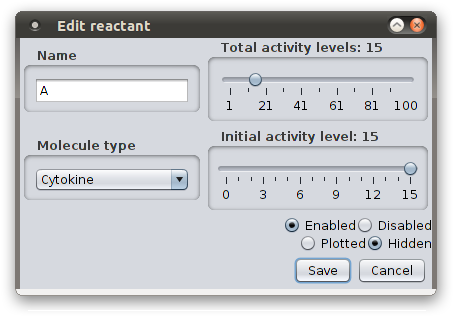
\includegraphics[width=.5\textwidth]{images/edit_reactantA}\\
 \caption{The \emph{Edit reactant} window: modifying the properties of node A.}\label{fig:edit-reactant}
\end{center}
\end{minipage}
\end{figure}


\begin{enumerate}
\setcounter{enumi}{\value{miocounterperenumerate}}
\item\label{step:add-edges} In order to add edges to the network, make sure that the \emph{Editor} tab is still active
in the \emph{Control Panel}, and
add the following edges by Ctrl-clicking the source and then clicking the target: A~$\rightarrow$~B, B~$\rightarrow$~C,
C~$\rightarrow$~B, B~$\rightarrow$~D, E~$\rightarrow$~D.
\item The \emph{Edit reaction} dialogue window is opened when you add a new edge,
or when you right click an existing edge and then select the \emph{[ANIMO] Edit reaction\dots} item
from the menu. Use that window to set the parameters of the edges as indicated in Table~\ref{tab:setting-edges}. The settings
for the edge A $\rightarrow$ B should reflect the ones shown in the \emph{Edit reaction} window in Figure~\ref{fig:edit-reaction}.\\
\emph{Note}: In order to insert a qualitative parameter like the ones required by the example network,
click once the slider in the \emph{parameter} box to activate it, and then move the slider to match the requested value.
\setcounter{miocounterperenumerate}{\value{enumi}}
\end{enumerate}

\begin{table}[!ht]
\begin{minipage}{\textwidth}
\processtable{The settings for the edges (interactions) in the example.\label{tab:setting-edges}}
{\begin{tabular}{llll}%|c|c|c|c|}
\hline\noalign{\vskip 2mm}
  {\bfseries Interaction} & {\bfseries Scenario} & {\bfseries Parameter value} & {\bfseries Influence}\\[2mm]
\hline
\noalign{\vskip 2mm}  A $\rightarrow$ B & 1 & Fast & Activation\\[5mm]
\noalign{\vskip 2mm}  B $\rightarrow$ C & 1 & Medium & Activation\\[5mm]
\noalign{\vskip 2mm}  C $\rightarrow$ B & 1 & V. Fast & Inhibition\\[5mm]
\noalign{\vskip 2mm}  B $\rightarrow$ D & 1 & Medium & Activation\\[5mm]
\noalign{\vskip 2mm}  E $\rightarrow$ D & 2 & 0.00015 & Inhibition\\[2mm]
\hline
\end{tabular}}{}
\end{minipage}
\end{table}\vspace{-2ex}

\begin{figure}[!tpb]
\begin{minipage}{\textwidth}
\begin{center}
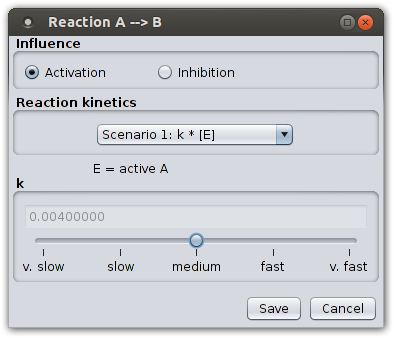
\includegraphics[width=.5\textwidth]{images/edit_reactionAB}\\
\caption{The \emph{Edit reaction} window: modifying the properties of edge A $\rightarrow$ B.}\label{fig:edit-reaction}
\end{center}
\end{minipage}
\end{figure}

\begin{enumerate}
\setcounter{enumi}{\value{miocounterperenumerate}}
\item In the \emph{Control Panel} activate the \emph{ANIMO} tab by clicking its title.
\item Click the \emph{Choose seconds/step} button. A new dialogue window will appear: you can
%just click \emph{OK} to confirm that you request a time resolution of 12 seconds.
safely choose a time resolution of 12 seconds per step and click \emph{OK}.
\item Click the \emph{Analyse network} button.
\item After a few seconds the \emph{Results Panel} should appear on the right,
showing a plot of the activity level of reactant D over a time course of 240 minutes.
Figure~\ref{fig:rete-esempio} shows the resulting network and graph plot.
\end{enumerate}

\begin{figure}[!tpb]
\begin{minipage}{\textwidth}
\begin{center}
  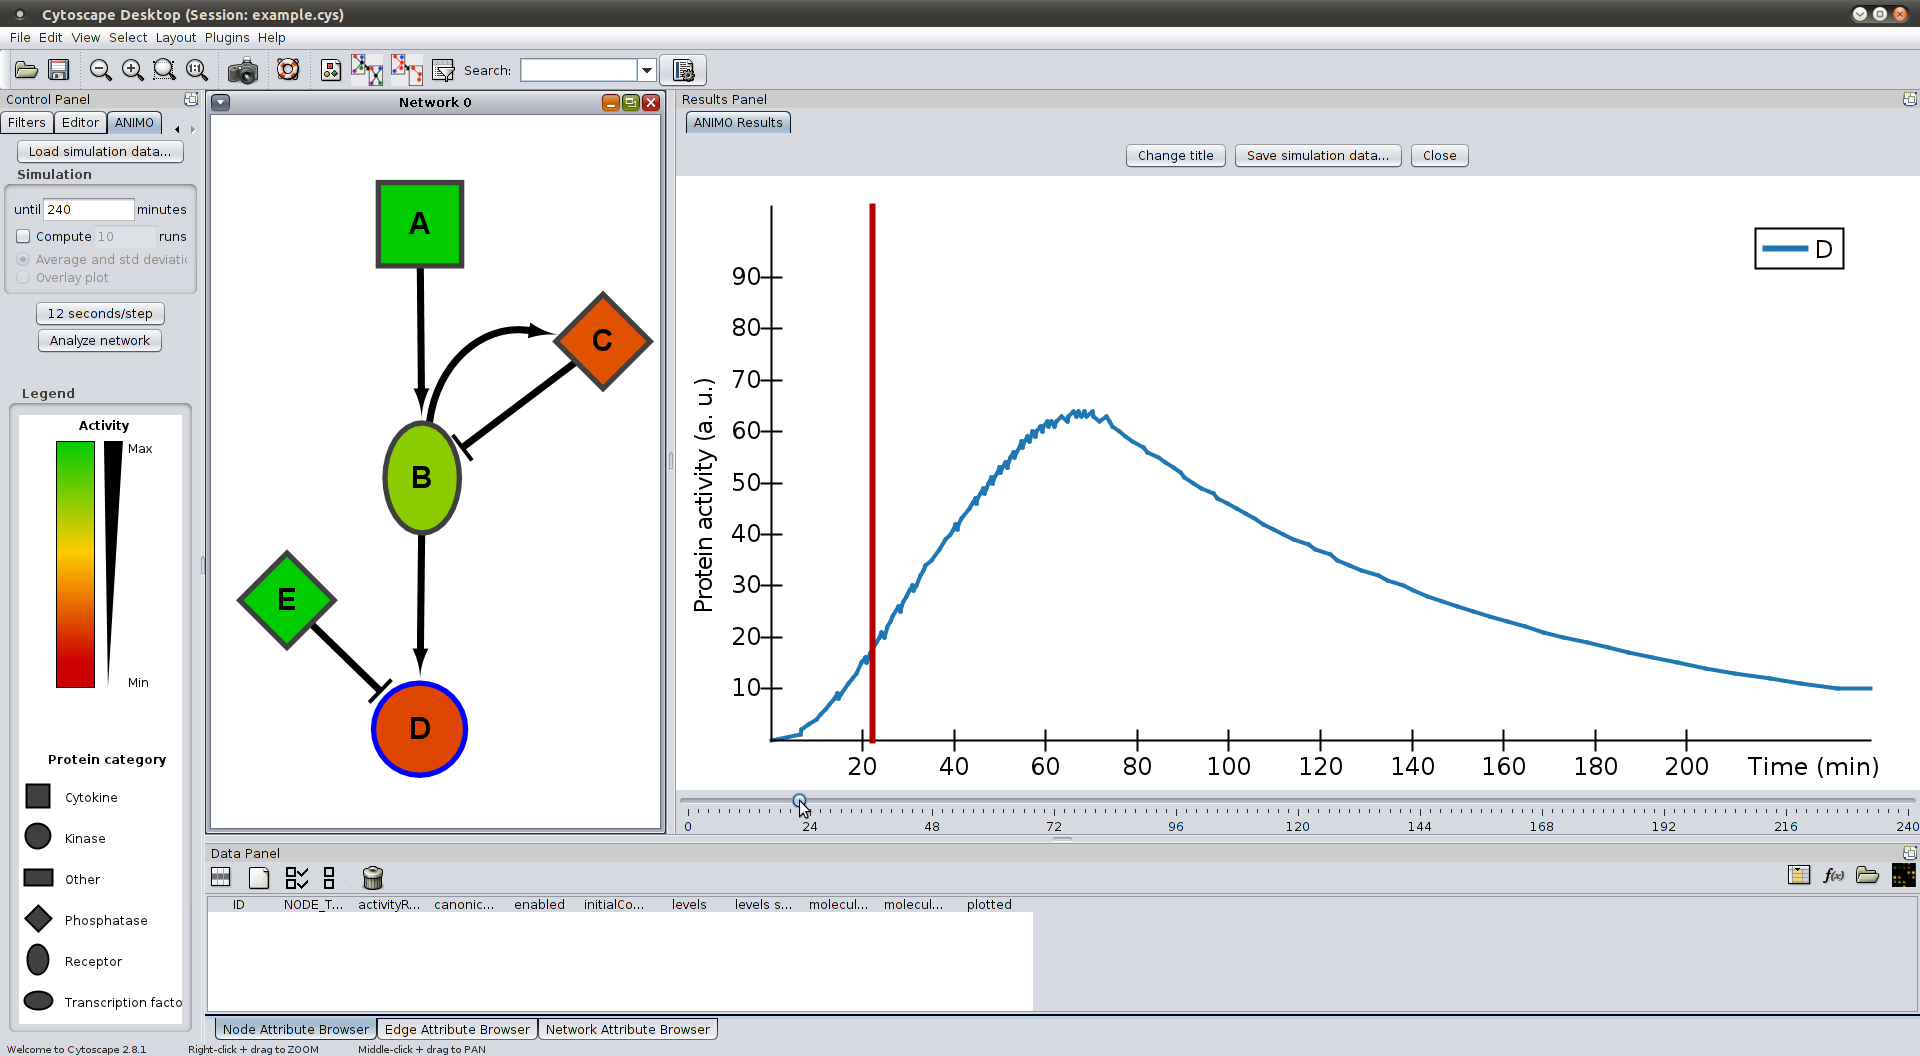
\includegraphics[width=.9\textheight, angle=90]{images/esempio_uso_ANIMO3}
\end{center}
\caption{The completed example, where also the feature that allows to view the activity levels
of reactants at chosen simulation times is demonstrated: the vertical red bar in the graph on the
right can be moved through the slider under the graph, and indicates the point in the time series
on which the colouring of the nodes in the \emph{Network} window is based.
The legends for colours and shapes can be found in the \emph{Legend} panel.}\label{fig:rete-esempio}
\end{minipage}
\end{figure}


\subsubsection{Managing simulation data and activity levels plots}
Each time a simulation result is obtained, a new tab is added to the \emph{Results Panel} (see the right part of Fig.~\ref{fig:rete-esempio})
in which we identify three buttons, a plot of the activity levels of the selected reactants and a time slider.

Clicking on the button \emph{Change title} allows to select a new title for the tab: this can be useful e.g. when comparing different
simulations made on similar configurations of the same network. Button \emph{Save simulation data\dots} allows to save
the simulation data of the current tab on a \emph{.sim} file, which can then be loaded and inspected in the future.
The \emph{Load simulation data\dots} button in the \emph{Control Panel} above the \emph{Simulation} box can be used for this purpose.
Please note that the best results are obtained only when loading a \emph{.sim} file when the \emph{Network} window contains the same network
on which the simulation data are based. If no network is currently opened, a network will \emph{not} be opened by loading a \emph{.sim} file.
The \emph{Close} button is used to close the currently displayed results tab.

Right clicking inside the graph area will bring up a menu that allows to perform some basic operations with the graph
and its data:
\begin{itemize}
  \item \emph{Add data from CSV}: \label{csv-import-format}superpose the graph with other data series found in a \emph{.csv} (comma separated values) file. This file type can be
obtained for example by exporting data from the default Excel format. If you want the data in the \emph{.csv} file to be rescaled so
that its maximum Y value coincides with the maximum in the plot, the data file needs to contain a column named (exactly)
\emph{Number\_{}of\_{}levels}, on the first row of which the maximum of the scale for the \emph{.csv} data needs to be put. For example,
if the data in the \emph{.csv} file are on a 0-100 scale, the value for \emph{Number\_{}of\_{}levels} will be 100.
  \item \emph{Save as PNG}: save the graph as it is shown in a \emph{.png} image file. This file format can be opened by most
image editors.
  \item \emph{Export visible as CSV}: export to a \emph{.csv} file all the series that are currently visible (i.e., not hidden)
in the graph.
  \item \emph{Clear Data}: clear the contents of the graph, removing all series. This can be useful for plotting
a \emph{.csv} file without superposing it to the current graph, or for loading a file in which all hidden data where removed
(exporting the visible graph to a \emph{.csv} with the previous command).
  \item \emph{Graph interval}: change the lower and upper bounds for X and Y axes.
  \item \emph{Zoom rectangle}: zoom the graph around a user-chosen rectangular area.
    After selecting this command the shape of the mouse cursor changes into a cross. The area of the plot to be
    zoomed can then be selected by dragging a rectangular selection around it (see the definition of \emph{rectangular
    selection} on page~\pageref{nota:rectangular-selection}).
  \item \emph{Zoom extents}: bring the zoom level back to default, cancelling the effects of any \emph{Zoom rectangle}
command.
\end{itemize}

Whenever the result of one or more simulations is shown as a graph, it is possible to use the slider under the graph to
move through the entire simulation, showing the activity levels of all reactants represented with different node colouring in
the \emph{Network} window on the left. For an example, see Figure~\ref{fig:rete-esempio}: the vertical red line in the
graph represents the time instant on which the colours of the nodes in the \emph{Network} window are based, and can
be moved with the slider over which the mouse cursor is drawn.




\subsection{Additional tips}
\subsubsection{Editing a network in Cytoscape}
Nodes and arcs can be placed in the network as shown previously: with the \emph{Editor} tab selected in the
\emph{Control Panel},
Ctrl-click (click while holding the {\tt Ctrl} or \maccmd\ key) in an empty place to add a node; Ctrl-click the source
node and click the target node to add an arc. It is also possible to drag and drop the node/arc icons from the \emph{Control Panel}
into the \emph{Network} window.\\
\emph{Note}: to perform \emph{drag and drop} move the mouse cursor over the icon in the \emph{Control Panel}, click with the left mouse
button and, without releasing the button, drag the mouse cursor on the \emph{Network} window where you want to
place the symbol; then release the left mouse button.

In order to delete a node/edge, select it by clicking
or grouping them in a larger rectangular selection, and then press the \emph{Delete} key on the keyboard
or select the \emph{Edit} $\rightarrow$ \emph{Delete Selected Nodes and Edges} menu command.\\
\emph{Note}: in order to obtain a \emph{rectangular selection}\label{nota:rectangular-selection},
left click in the \emph{Network} window where the upper-left corner of the rectangle should be and,
without releasing the left mouse button, drag the mouse cursor to where the lower-right corner of the
rectangular selection should be; then release the left mouse button. All the entities which were
\emph{even partially} touched by the rectangle are now selected.

Navigation inside the \emph{Network} window can be performed by clicking and dragging the centre mouse button,
while zooming can be done by either rotating the mouse wheel or clicking and holding the right mouse button
while moving the mouse in a vertical direction.

Finally, note that the colours used to represent node activity can be changed using the \emph{VizMapper}
interface provided by Cytoscape, changing the setting for \emph{Node colour}, shown in Figure~\ref{fig:change-gradient}.
To change the node colours, activate the \emph{VizMapper\texttrademark} tab in the \emph{Control Panel}, and
find the entry named \emph{Node Colour} in the \emph{Visual Mapping Browser} box. Click the arrow-shaped
icon directly to the left of \emph{Node Colour}: the current setting for the node colours should appear:
click the coloured bar to open the window shown in Figure~\ref{fig:change-gradient}.
The \emph{activityRatio} on which the node colouring is based is the ratio between the current activity level
of a node and its number of activity levels.
The coloured arrows pointing downward on the upper border of the coloured rectangle can be dragged along the length of the $[0, 1]$
interval, thus changing the point at which a particular colour appears. New arrows can be added with the \emph{Add} button, while
clicking an arrow and pressing the \emph{Delete} button will remove one. To change the colour of a point in the interval,
double click the corresponding arrow, and a new window will open, allowing you to choose a new colour: clicking \emph{OK} will
accept the new colour. The modifications made in the \emph{Gradient Editor for Node Colour} window should be automatically reflected in
the model: when the gradient is as wanted, simply close the window. If the node colours seem not to have been updated, please move the
slider under an existing graph in the \emph{Results Panel}.

\begin{figure}[!tpb]
\begin{minipage}{\textwidth}
\centering
  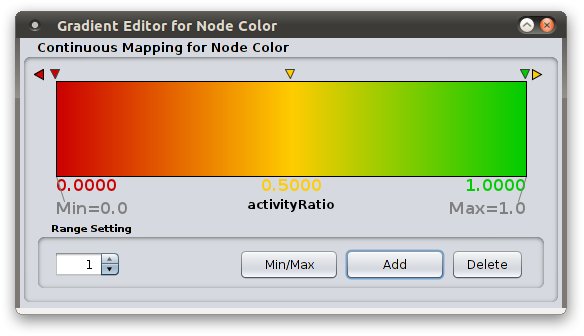
\includegraphics[width=.6\textwidth]{images/editing-gradient2}
  \caption{Changing the colours used to represent node activity in an ANIMO model.}\label{fig:change-gradient}
\end{minipage}
\end{figure}


\subsubsection{ANIMO features}
Nodes and edges (and groups of nodes/edges highlighted via a rectangular selection)
can be disabled by choosing \emph{[ANIMO] Enable/disable} from
the right-click menu: they will be represented with less saturated colours and can be re-enabled by performing
the same action. Moreover, a node can be enabled/disabled directly in its properties window, where it is
also possible to add/remove the node from the list of series appearing in the graph resulting from a simulation
of the network by selecting \emph{Plotted} or \emph{Hidden} (see also Figure~\ref{fig:edit-reactant}):
nodes that will be plotted are circled in blue.
Every enabled node will be taken into account when computing the evolution of the system,
but only nodes marked as \emph{Plotted} will appear in a graph.

Each plot in an \emph{ANIMO Results} tab contains by default a legend, which can be used to modify which series are
displayed and how they are displayed. Clicking with the central mouse button on a series name will hide it from the
graph, while the same centre-click the coloured line beside the series name will change the colour of that series,
cycling through a predefined set of available colours. The entire legend can be hidden by clicking with the
central mouse button anywhere on the graph (not inside the legend), or it can be dragged around by clicking and holding the left
mouse button, releasing it when the preferred position is reached. Rotating the mouse wheel will allow the thickness of all
the graph lines, and the size of the text, to grow or decrease: this feature can be useful when the window containing
the graph is very large.

As the model is non-deterministic, i.e. its
evolution will not be exactly the same for every single simulation run, it is possible to ask ANIMO to perform
a number of simulation runs in a batch, plotting the averages of the activity levels over the runs together with a standard
deviation value, or showing a so-called \emph{overlay plot} where all runs are plotted over each other. The controls
that allow to ask for multiple simulation runs can be found in the \emph{Control Panel}, inside the \emph{Simulation} box.

Standard deviation may be represented in the graph: it is normally shown as vertical bars, but its aspect can be
cycled through five possibilities (vertical bars, shading, both bars and shading, bars and symbols, none) by right-clicking the
corresponding line in the legend. Symbols associated to a representation of standard deviation can be changed by Shift-right-clicking
(holding down the \emph{Shift} key, right click) on the corresponding line in the legend.
Standard deviation values can be obtained when asking for multiple simulations in the network
analysis, but they can also be present in a \emph{.csv} file, e.g. when the file contains averages of experimental data.
In a \emph{.csv} file, the column containing the standard deviation values for column \emph{A}
should be named \emph{A\_{}StdDev} for the program to recognize it and properly display the data series
with the associated error values.



\subsubsection{Parameter settings}
The application of some basic strategies when setting the parameters for a network allows
the less experienced users to considerably shorten the modelling time.
First of all, it is important to proceed in a \emph{top-to-bottom} order, trying to match
a component to the corresponding data before inserting the components downstream thereof.
Second, when choosing the kinetic parameter for an interaction, we advise to first use the qualitative settings (very slow, slow, medium, fast, very fast):
this allows to define the relative speeds of the interactions as soon as possible,
leaving the more precise parameter setting procedure as a follow-up step. Finally, as can be seen from
the parameter settings of Section~\ref{sec:modeling-network-example}, in order to obtain a peak
behaviour it is particularly important that
a negative feedback is present (as an example, see the interactions involving B and C in Tab.~\ref{tab:setting-edges}),
and that the inactivating interaction in the loop is faster than the ones activating the target node.

A final note on the \emph{seconds/step} button. This button allows to define the time granularity
of the simulations, but it is not strictly necessary to choose a very precise value.
% As the time bounds in the \tas\ model are integers, rounding errors can make the model
% behave differently from what the parameters define.
If the current value for \emph{seconds/step}
is too high (or too low) to allow the network to be properly simulated, ANIMO will automatically choose (respectively)
the highest (lowest) value that still allows to avoid rounding problems. It will be possible to notice
such a change in the value of time scale when the number on the \emph{seconds/step} button changes.


\subsubsection{Updating ANIMO}
To check whether a new version of ANIMO has been published, run Cytoscape and ask for an update of all
plug-ins via the menu command \emph{Plugins} $\rightarrow$ \emph{Update Plugins}. After some seconds
during which Cytoscape will contact all the providers of the installed plug-ins,
the system should report the list of updatable plug-ins.\\
\emph{Note}: a window with the message \emph{Attempting to connect to XYZ\dots} may appear and disappear multiple times:
it is the normal behaviour.

If an updated version of ANIMO is available, it will appear
under the category \emph{Updatable Plugins} $\rightarrow$
\emph{Analysis} $\rightarrow$ \emph{ANIMO v1.28}. If no plug-in can be updated, a message stating \emph{No
updates available for currently installed plug-ins.} will be shown.




\clearpage
\section{Naming conventions}\label{suppl-sec:names}
Table~\ref{suppl-tab:names} explains the abbreviations used in the paper.

\begin{center}
\begin{longtable}{lll}
\caption{Explanation of the abbreviated names referring to molecular species
in the main text.}\label{suppl-tab:names} \\
%\begin{tabular}{lll}
\hline
\noalign{\vskip 2mm} {\bfseries Abbreviation} & {\bfseries Full name} \\[2mm]
\hline
\endfirsthead

\multicolumn{3}{c}%
{\scriptsize{\bfseries \tablename\ \thetable{}} \--\ continued from previous page} \\
\hline
\noalign{\vskip 2mm} {\bfseries Abbreviation} & {\bfseries Full name} \\[2mm]
\hline
\endhead

\hline \multicolumn{3}{r}{{Continued on next page}} \\ %\hline
\endfoot

\hline
\endlastfoot

\noalign{\vskip 2mm}  Akt & protein kinase B & \\
\noalign{\vskip 2mm}  AP-1 & activator protein 1 \\
\noalign{\vskip 2mm}  Casp3 & caspase 3 & \\
\noalign{\vskip 2mm}  Casp8 & caspase 8 & \\
\noalign{\vskip 2mm}  c-Fos & proto-oncogene-protein c-fos & \\
\noalign{\vskip 2mm}  c-Jun & Jun activation domain binding protein & \\
\noalign{\vskip 2mm}  CLK & clock & \\
\noalign{\vskip 2mm}  CRY & cryptochrome & \\
\noalign{\vskip 2mm}  CWO & clockwork orange & \\
\noalign{\vskip 2mm}  CYC & cycle & \\
\noalign{\vskip 2mm}  CYC/CLK & cycle-clock complex & \\
\noalign{\vskip 2mm}  DBT & double-time kinase & \\
\noalign{\vskip 2mm}  DISC1 & death-inducing signalling complex 1 & \\
\noalign{\vskip 2mm}  DISC2 & death-inducing signalling complex 2 & \\
\noalign{\vskip 2mm}  EGF & epidermal growth factor & \\
\noalign{\vskip 2mm}  EGFR & EGF receptor & \\
\noalign{\vskip 2mm}  ERK & extracellular regulated kinase & \\
\noalign{\vskip 2mm}  FKHR & forkhead box protein O1 & \\
\noalign{\vskip 2mm}  IKK & inhibitor of nuclear factor kappa-B kinase & \\
\noalign{\vskip 2mm}  IL-1a & interleukin 1 $\alpha$ & \\
\noalign{\vskip 2mm}  IL-1R & interleukin 1 receptor & \\
\noalign{\vskip 2mm}  IL-1ra & interleukin 1 receptor antagonist & \\
\noalign{\vskip 2mm}  IRS1 (S) & insulin receptor substrate 1 (Serine 636) & \\
\noalign{\vskip 2mm}  IRS1 (Y) & insulin receptor substrate 1 (Tyrosine 896) & \\
\noalign{\vskip 2mm}  JNK1 & c-Jun N-terminal kinase 1 & \\
\noalign{\vskip 2mm}  MEK & MAPK ERK kinase & \\
\noalign{\vskip 2mm}  MEKK1 & MAPK/ERK kinase kinase 1 & \\
\noalign{\vskip 2mm}  MK2 & mitogen-activated protein kinase-activated protein kinase 2 & \\
\noalign{\vskip 2mm}  MKK3/6 & dual specificity mitogen-activated protein kinase kinase 3/6 & \\
\noalign{\vskip 2mm}  MKK4/7 & dual specificity mitogen-activated protein kinase kinase 4/7 & \\
\noalign{\vskip 2mm}  NF-kB & nuclear factor kappa-B & \\
\noalign{\vskip 2mm}  p38 & mitogen-activated protein kinase p38 & \\
\noalign{\vskip 2mm}  PDP1 & par-domain protein 1 & \\
\noalign{\vskip 2mm}  PER & period & \\
\noalign{\vskip 2mm}  PER/TIM-p & phosphorylated period-timeless complex & \\
\noalign{\vskip 2mm}  RAF & Raf & \\
\noalign{\vskip 2mm}  RAS & Ras GTPase-activating protein & \\
\noalign{\vskip 2mm}  TGF$\alpha$ & transforming growth factor $\alpha$ & \\
\noalign{\vskip 2mm}  TNF$\alpha$ & tumour necrosis factor-$\alpha$ & \\
\noalign{\vskip 2mm}  TNFR & TNF receptor & \\
\noalign{\vskip 2mm}  TIM & timeless & \\
\noalign{\vskip 2mm}  VRI & vrille & \\[2mm]
\hline
%\end{tabular}
\end{longtable}
\end{center}




\clearpage
\section{Normalizing experimental data for use with ANIMO}\label{suppl-sec:normalization}
Document S1 in the Supplemental Data of the work by~\citet{pathway-autocrine} contains
three tables, named {\sf Replicates}, {\sf Averages} and {\sf DPLSR dataset}.
The data we use to compare the results computed with ANIMO are based on the 
values from the {\sf Averages} table.
In particular, we compute activity data by performing a normalization on a $0\dots 100$ scale using this formula
$$
v_{\mbox{\scriptsize norm}} = \frac{v}{v_{\mbox{\scriptsize max}}} \times 100
$$
where $v$ is the datum to be normalized taken from the column $v$ in the {\sf Averages} table,
$v_{\mbox{\scriptsize norm}}$ is the normalized value and
$v_{\mbox{\scriptsize max}}$ is the maximum value over the whole column $v$ in the {\sf Replicates} table.
For each series, we compute also the standard deviation using the triplicate measurements
present in table {\sf Replicates}. The standard deviation is also normalized using the formula presented for the average.
Each table produced with this process contains a subset of the columns from the {\sf Averages} table,
and refers to one treatment condition only. A column with time references is added to the table in first position.
Finally, a column named \emph{Number\_of\_levels} containing only the value $100$ (see the instructions
on page~\pageref{csv-import-format}) is added at the rightmost position.
The tables are all exported in .csv format to be used with ANIMO, and are included in the \emph{Model\_and\_data.zip}
file in the additional materials of the present work.


\clearpage
\section{ANIMO and Timed Automata}\label{suppl-sec:animo-ta}

\subsection{Timed Automata model}
The Timed Automata (\tas) model underlying an ANIMO network is generated whenever an analysis is requested by the user.
Starting from the network represented in the Cytoscape-based user interface, ANIMO automatically generates a \tas\ model
to be used with UPPAAL. The analysis result is then parsed and properly presented to the user, for example
as a graph of reactant activity levels. This workflow is described in Figure~\ref{fig:animo-sim-workflow}.

\begin{figure}[htb]
\begin{minipage}{\textwidth}
  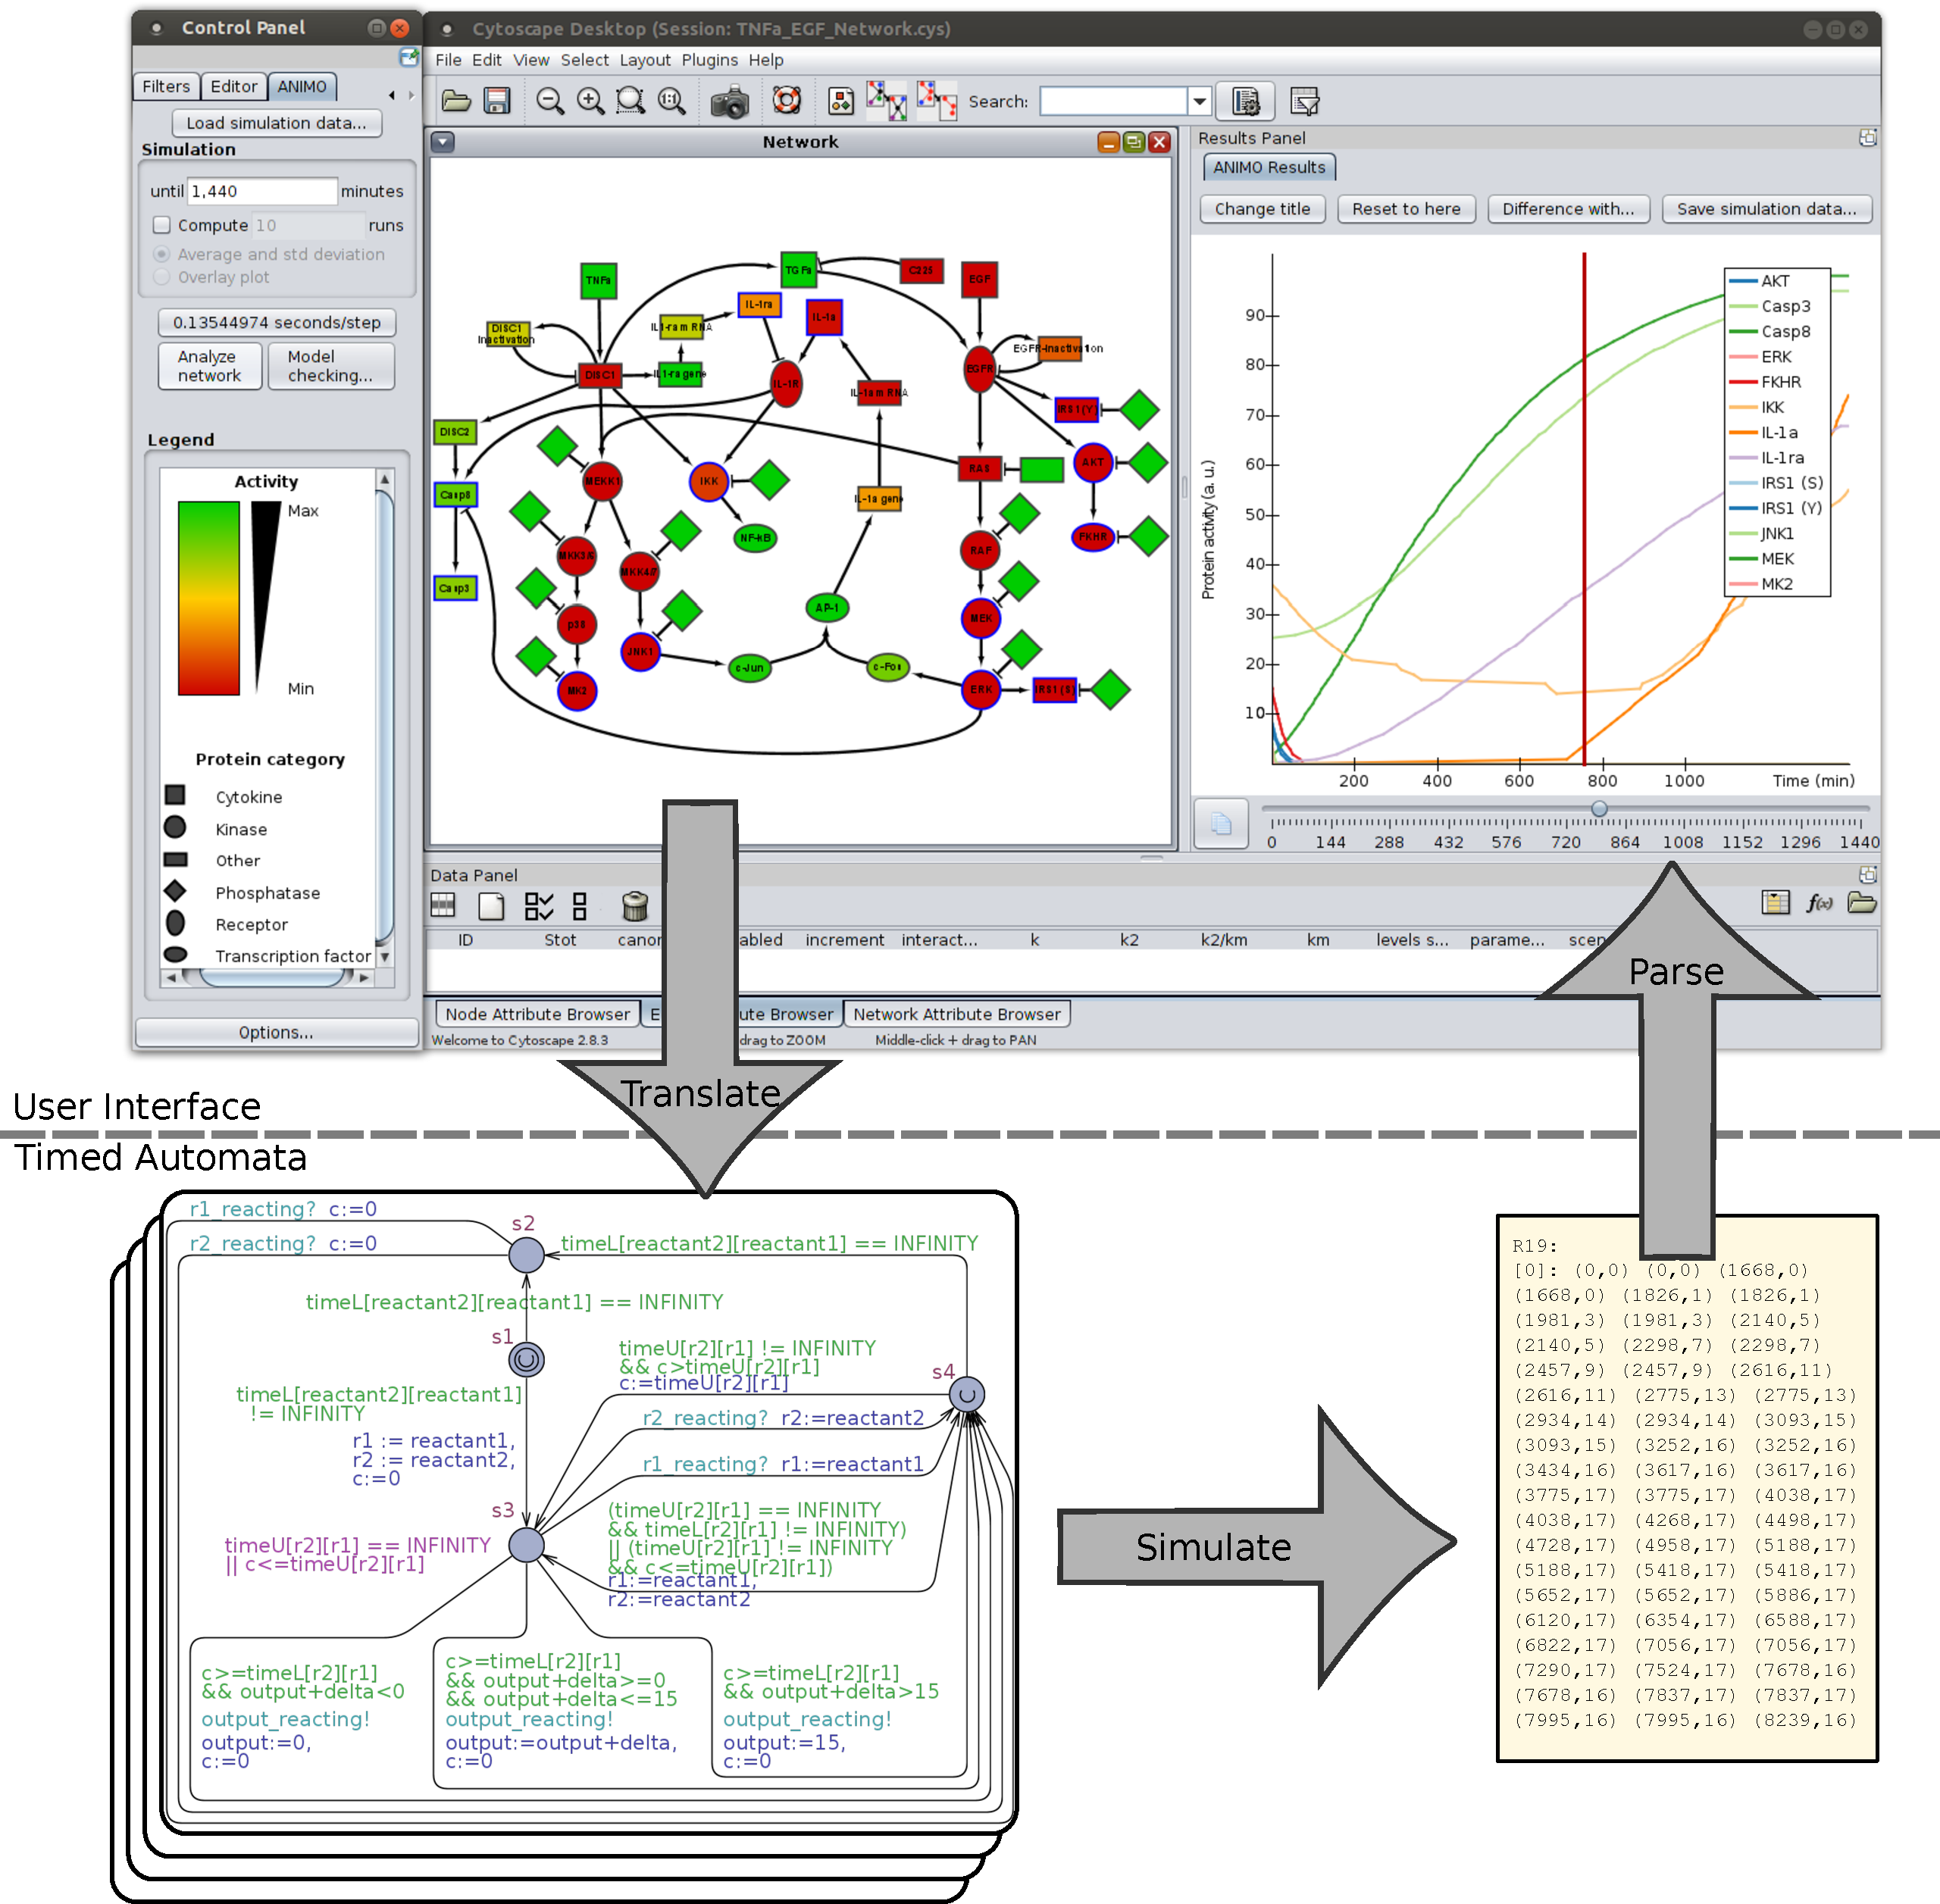
\includegraphics[width=\textwidth]{images/animo_simulation_workflow}
\caption{The passages intercurring between the press of the \emph{Analyse network} button
and the generation of an activity level graph.
A simulation produces, for each selected node, a series of pairs {\sf ($t$, $a$)},
with $t$ a time instant along the simulation and $a$ an activity level. These data are
then parsed and translated into a graph.}\label{fig:animo-sim-workflow}
\end{minipage}
\end{figure}

Each \tas\ model generated by ANIMO contains one automaton for each interaction (activation or inhibition) in the network.
A \ta\ representing an interaction performs a cyclic series of steps, continuously updating
the target of the interaction it represents, and adapting the timing of the next update according to
the user-defined dynamics. Synchronizations between different automata occur when the activity level of a network component (e.g. ERK)
changes: this allows the automata depending on that component to update their time settings.

The abstract behaviour of the interaction $\mbox{MEK} \rightarrow \mbox{ERK}$ in the \tas\ model used in ANIMO is described in Figure~\ref{fig:ta-diagram}.
There, the activity levels of MEK and ERK are represented by variables called, respectively, $\mbox{MEK}_{\mbox{\scriptsize activity}}$
and $\mbox{ERK}_{\mbox{\scriptsize activity}}$. A more detailed description of the \tas\ model underlying ANIMO has been presented
at the IEEE conference BIBE 2012~\citep{animo-bibe}.

\tikzstyle{decision} = [rectangle, draw, fill=yellow!20, text width=.45\textwidth, text badly centered]
\tikzstyle{block} = [rectangle, draw, fill=blue!20,
    text width=.45\textwidth, text centered, rounded corners, minimum height=4em]
\tikzstyle{line} = [draw, thick, -latex']
\tikzstyle{cloud} = [draw, ellipse,fill=blue!20, minimum height=2em]
\def\svgwidth{.8\textwidth}
\definecolor{lowActivity}{rgb}{0.8,0,0}
\definecolor{highActivity}{rgb}{0,0.8,0}%{1,0.8,0}
\newsavebox{\mysquareLow}
\savebox{\mysquareLow}{%
  \raisebox{-0.08em}{%
    \textcolor{black}{%
      \rule{.7em}{.7em}%
    }%
    \hspace{-.65em}%
    \raisebox{.05em}{%
      \textcolor{lowActivity}{%
	\rule{.6em}{.6em}%
      }%
    }%
  }%
}
\newsavebox{\mysquareHigh}
\savebox{\mysquareHigh}{%
  \raisebox{-0.08em}{%
    \textcolor{black}{%
      \rule{.7em}{.7em}%
    }%
    \hspace{-.65em}%
    \raisebox{.05em}{%
      \textcolor{highActivity}{%
	\rule{.6em}{.6em}%
      }%
    }%
  }%
}

\begin{figure}[!ht]
\begin{minipage}{\textwidth}
\centering

\begin{tikzpicture}[node distance = 2cm, auto, scale=0.8, every node/.style={scale=0.8}]
    % Place nodes
    \node [block] (init) {
\begingroup
  \makeatletter
  \providecommand\color[2][]{%
    \errmessage{(Inkscape) Color is used for the text in Inkscape, but the package 'color.sty' is not loaded}
    \renewcommand\color[2][]{}%
  }
  \providecommand\transparent[1]{%
    \errmessage{(Inkscape) Transparency is used (non-zero) for the text in Inkscape, but the package 'transparent.sty'
is not loaded}
    \renewcommand\transparent[1]{}%
  }
  \providecommand\rotatebox[2]{#2}
  \ifx\svgwidth\undefined
    \setlength{\unitlength}{1974.66679688pt}
  \else
    \setlength{\unitlength}{\svgwidth}
  \fi
  \global\let\svgwidth\undefined
  \makeatother
  \begin{picture}(1,0.37)%26031697)%
    \put(0,0){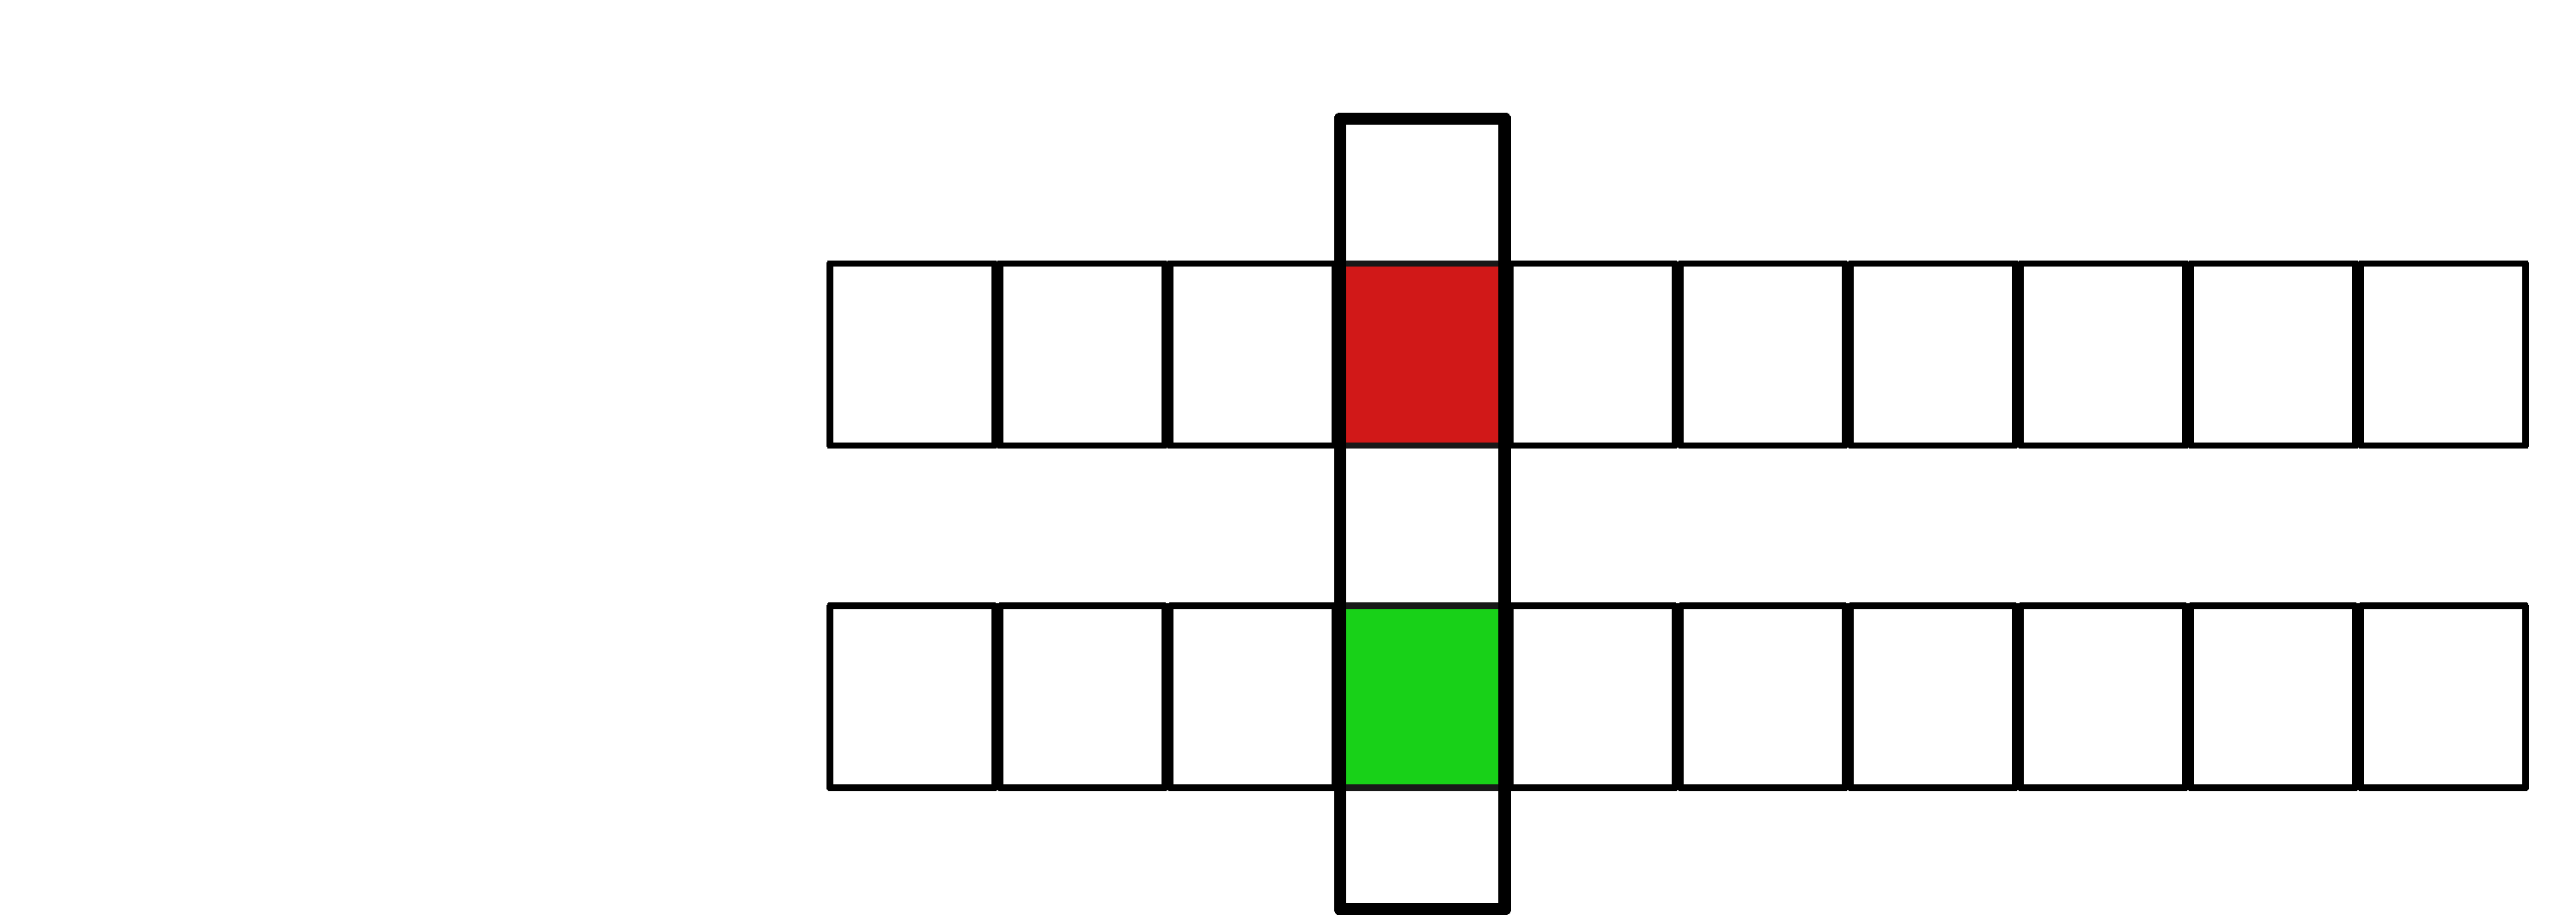
\includegraphics[width=\unitlength]{images/mek_activity_time_tables2.pdf}}%
    \put(0.005,0.20182345){\color[rgb]{0,0,0}\makebox(0,0)[lb]{\smash{$R_{\mbox{\scriptsize lowerBound}}$}}}%
    \put(0.005,0.07442319){\color[rgb]{0,0,0}\makebox(0,0)[lb]{\smash{$R_{\mbox{\scriptsize upperBound}}$}}}%
    \put(0.45,0.325)%23815501)
	{\color[rgb]{0,0,0}\makebox(0,0)[lb]{\smash{$\mbox{MEK}_{\mbox{\scriptsize
activity}}$}}}%
  \end{picture}%
\endgroup
};
    \node [block, above of=init, node distance=2.5cm] (reset) {Reset the internal clock: ${\sf t} \!\!:= \!\!0$};
    \node [cloud, above of=reset, node distance=1.5cm] (start) {Start};
\node [block, below of=init, node distance=2.5cm] (choose) {$R$ will occur when
\raisebox{-0.3ex}{\pgfuseimage{lower-bound}} $\leq\!\!\! {\sf t}\!\!\! \leq$
\raisebox{-0.3ex}{\pgfuseimage{upper-bound}}
    };
    \node [block, below of=choose] (increase) {Increase $\mbox{ERK}_{\mbox{\scriptsize activity}}$
by $+1$ level};
    \node [block, below of=increase] (inform) {Inform interactions depending on $\mbox{ERK}_{\mbox{\scriptsize
activity}}$\\
    of the change};
    % Draw edges
    \path [line] (start) -- (reset);
    \path [line] (reset) -- (init);
    \path [line] (init) -- (choose);
    \path [line] (choose.west) -| +(-0.5, 2) node [pos=0.78, sloped, above, align=left] {$\mbox{MEK}_{\mbox{\scriptsize activity}}$ was changed} |- (init.west);
    \path [line] (choose) -- (increase);
    \path [line] (increase) -- (inform);
    \path [line] (inform.east) -| +(1, 4) |- (reset.east);
\end{tikzpicture}
\caption{Schematic overview of the steps taken during a simulation run by a Timed Automaton modelling an interaction $R$ that
increases $\mbox{ERK}_{\mbox{\scriptsize activity}}$ and depends only on $\mbox{MEK}_{\mbox{\scriptsize activity}}$.
In this example, MEK has 10 activity levels.\\
After resetting the internal clock {\sf t}, the automaton sets the time constraints for the interaction.
$\mbox{MEK}_{\mbox{\scriptsize activity}}$ is used as the index inside the time
tables $R_{\mbox{\scriptsize lowerBound}}$ and $R_{\mbox{\scriptsize upperBound}}$, which contain pre-computed lower- and upper-bounds
for the interaction timing.
Once the bounds have been identified, %the internal clock {\sf t} begins counting.
$R$ can occur when {\sf t} reaches a value
inside the continuous time interval~$[\,\usebox{\mysquareLow}, \usebox{\mysquareHigh}\,]$. When it occurs, $R$ increases the value of
$\mbox{ERK}_{\mbox{\scriptsize activity}}$ by $1$. All interactions that depend on
$\mbox{ERK}_{\mbox{\scriptsize activity}}$ are notified of the change (via a synchronization on a specific channel),
so that the associated time bounds are updated accordingly.
After resetting the clock {\sf t}, the process can restart.
If $\mbox{MEK}_{\mbox{\scriptsize activity}}$ was changed by another automaton before the occurrence of $R$, 
the time bounds are updated according to the new activity level of MEK.}\label{fig:ta-diagram}
\end{minipage}
\end{figure}



\subsection{Granularity of an ANIMO network node}
Figure~\ref{fig:levels} shows the differences between different choices for the
number of levels of a node. This allows to adapt a model to the quality of experimental data.

\begin{figure}[htpb]
\begin{minipage}{\textwidth}
\centering
\subfloat[\label{suppl:fig1-1level}]{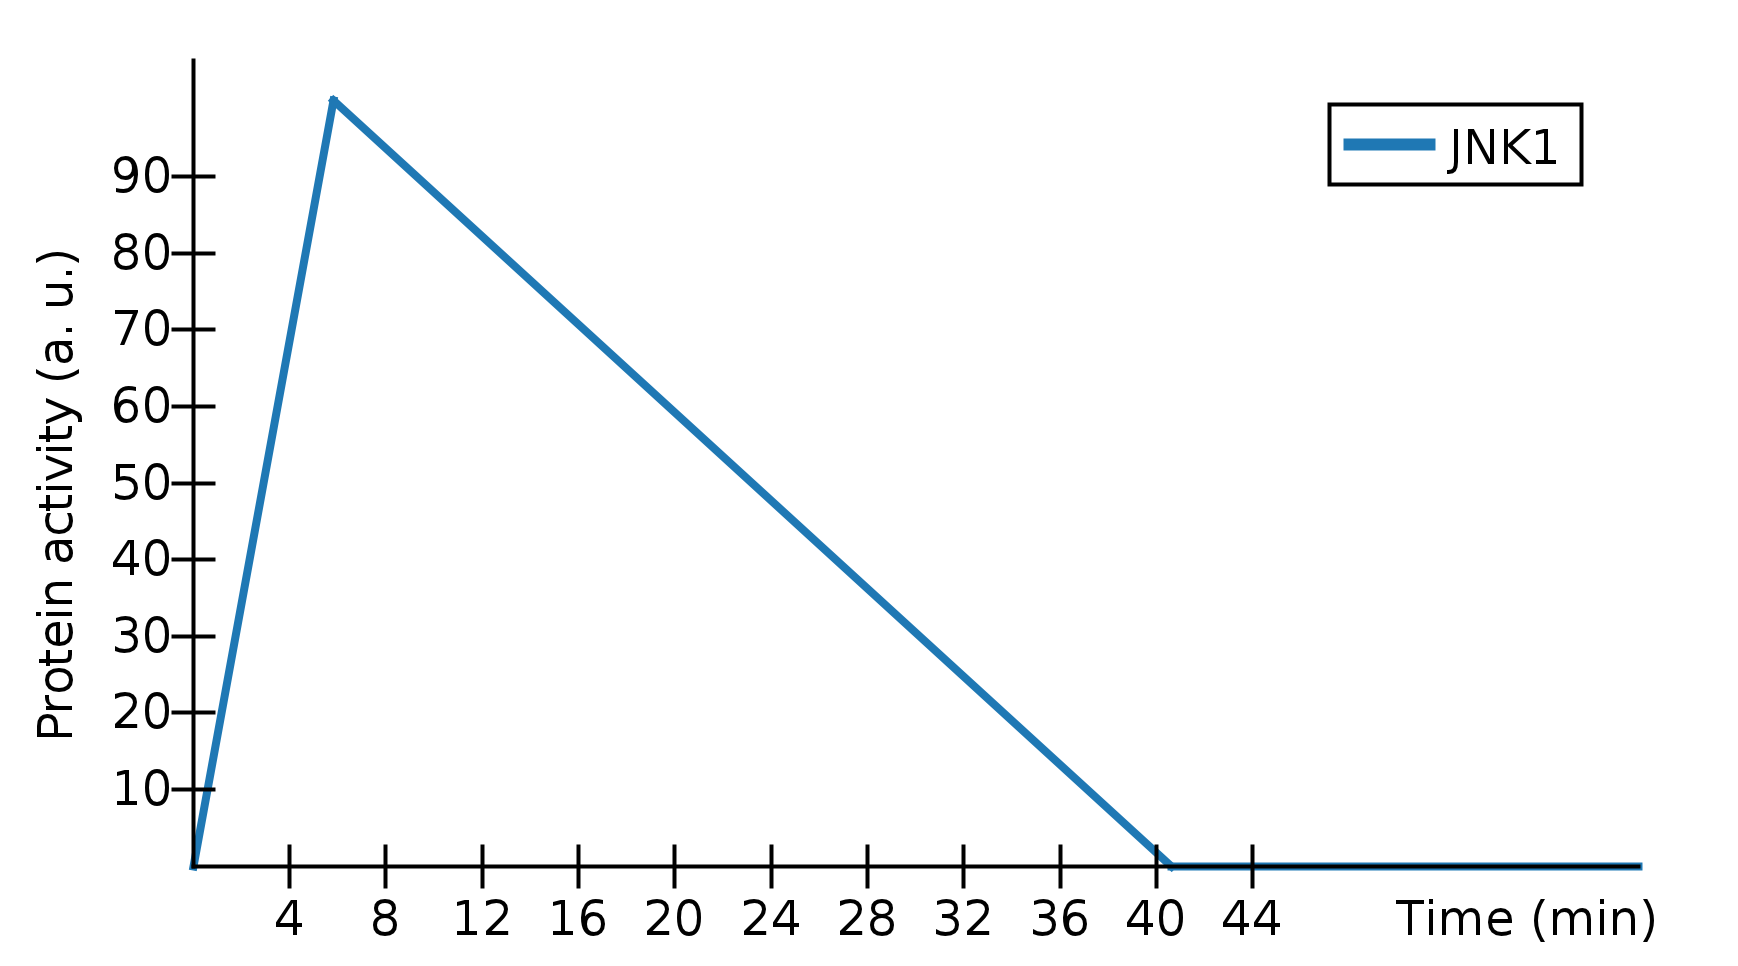
\includegraphics[width=.45\textwidth]{images/JNK1_1level2}} \qquad
\subfloat[\label{suppl:fig1-10levels}]{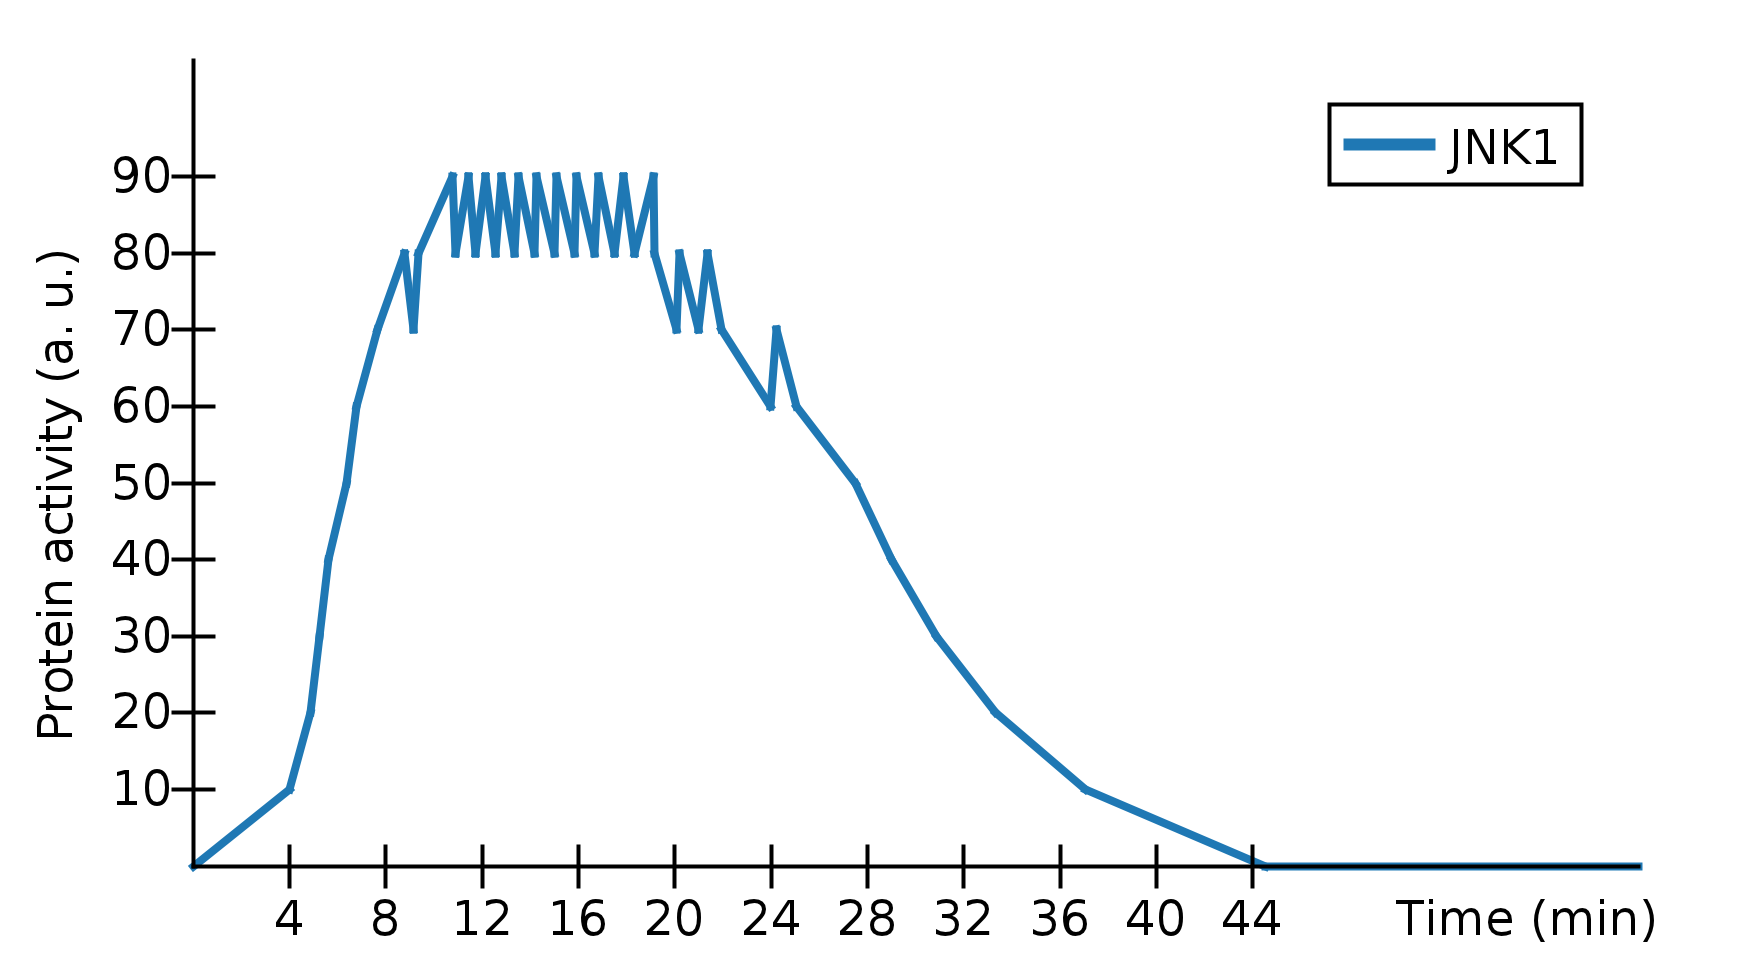
\includegraphics[width=.45\textwidth]{images/JNK1_10levels2}} \\
\subfloat[\label{suppl:fig1-50levels}]{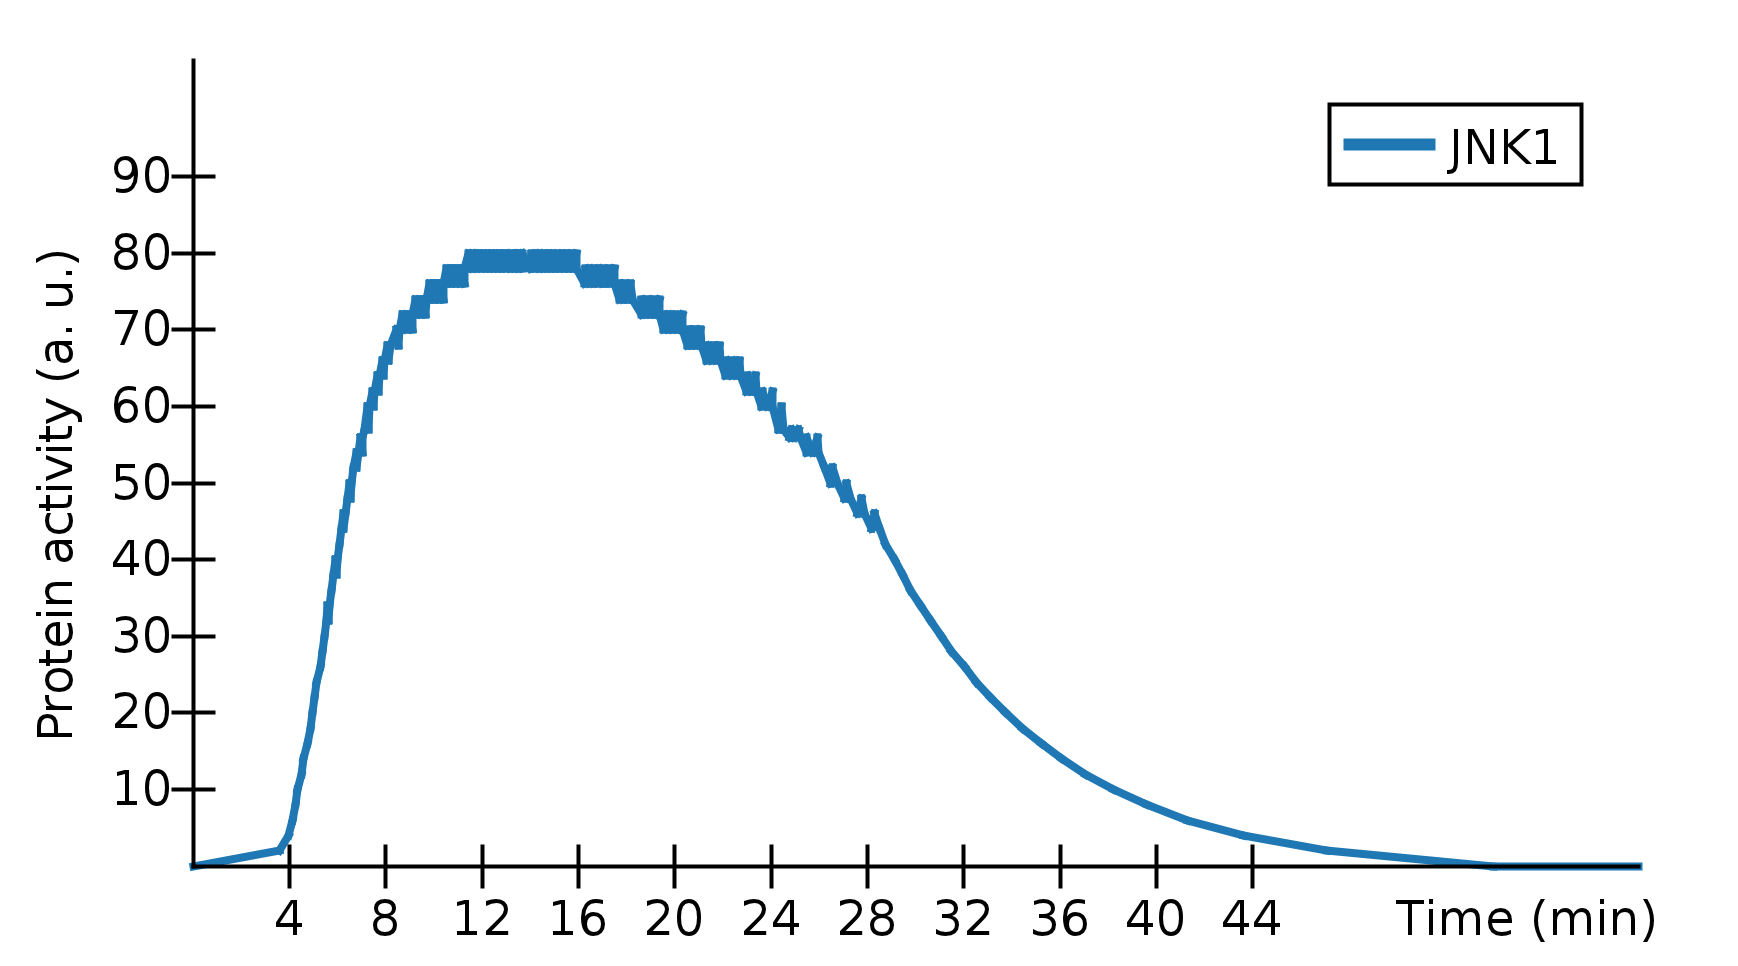
\includegraphics[width=.45\textwidth]{images/JNK1_50levels2}} \qquad
\subfloat[\label{suppl:fig1-100levels}]{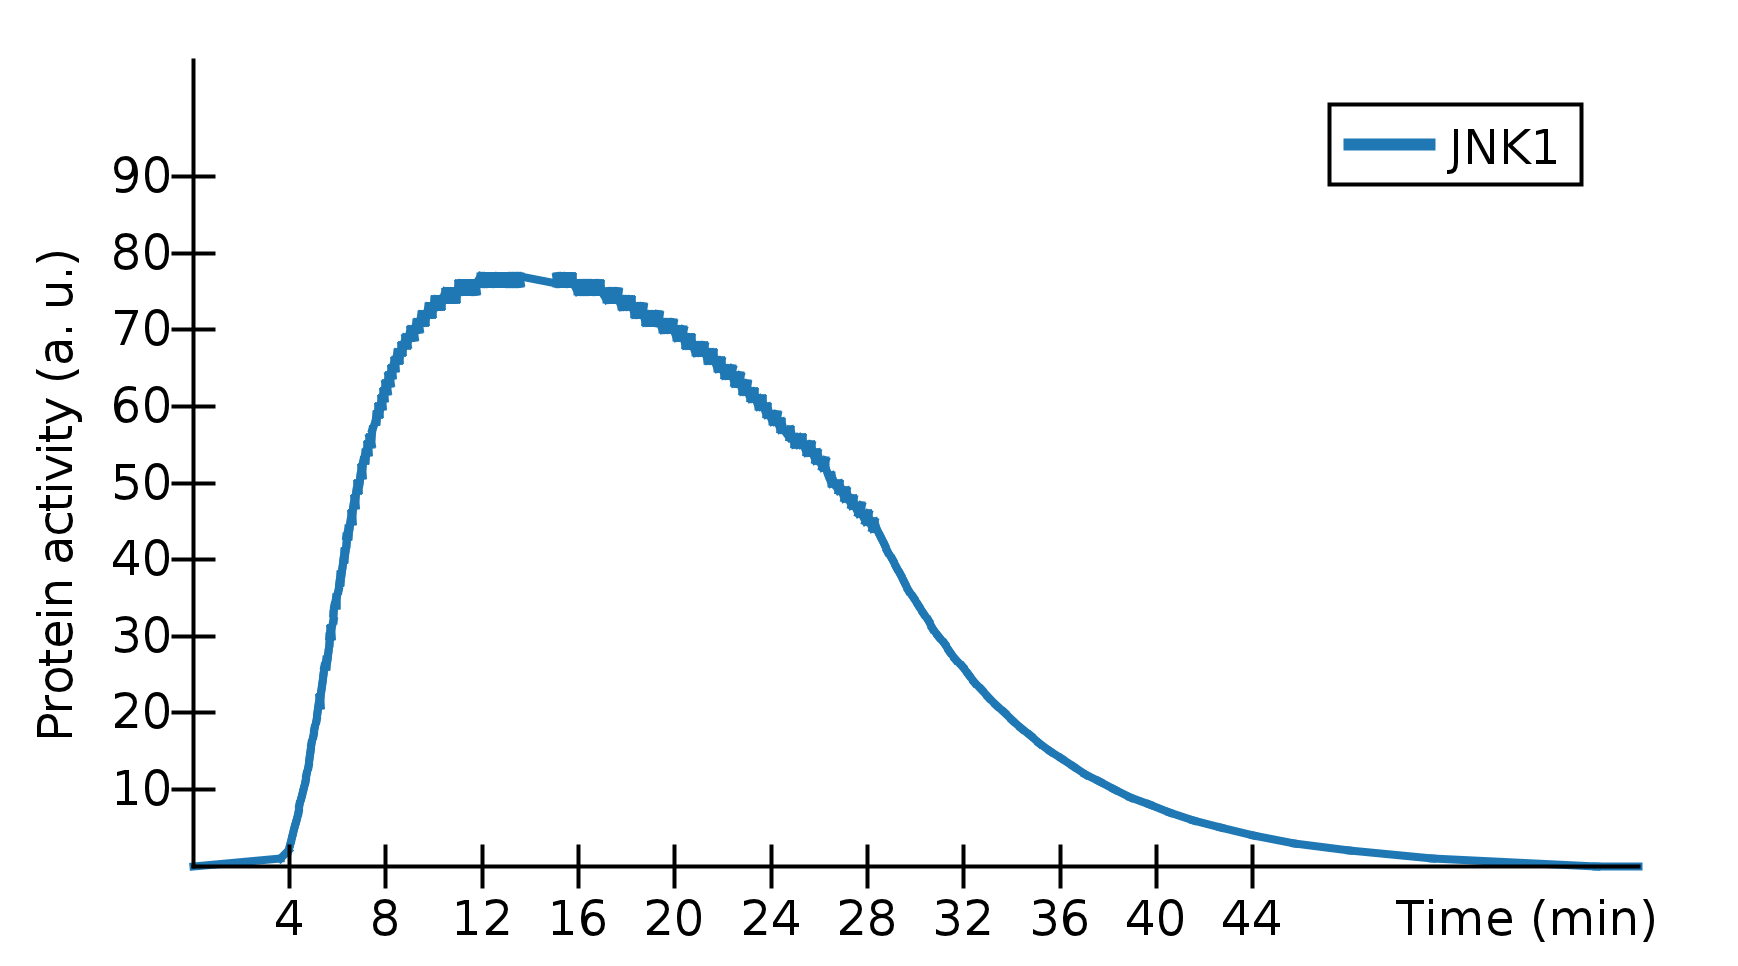
\includegraphics[width=.45\textwidth]{images/JNK1_100levels2}}
\caption{Comparing different reactant granularity settings. {\bfseries (\protect\subref*{suppl:fig1-1level})} 2 levels, {\bfseries (\protect\subref*{suppl:fig1-10levels})} 10 levels,  {\bfseries (\protect\subref*{suppl:fig1-50levels})} 50 levels, {\bfseries (\protect\subref*{suppl:fig1-100levels})} 100 levels. The {\sf JNK1} series is computed from the model presented in Figure~\ref{fig:large-model-complete}, considering 100 ng/ml TNF$\alpha$ as treatment condition over a period of 60 minutes.}\label{fig:levels}
\end{minipage}
\end{figure}



\clearpage
\section{Additional notes}

\subsection{Simulating the day-night cycle}\label{suppl:repressilator}
The model presented in Figure~\ref{subfig:drosophila-model} contains a node
labelled {\sf Day/Night}. That node abstracts our representation
of the cyclic alternation of day and night, which causes the variations
in cryptochrome ({\sf cry}): these oscillations allow the network
to synchronize to a time zone. Note that the network oscillates
also when the node {\sf cry} is not included in the model.

The alternation between day and night is represented in our model with a
repressilator-like~\citep{repressilator} subnetwork, as can be seen in Figure~\ref{fig:repressilator}.
In the model by~\cite{drosophila-ode-model} a specific function
was introduced in the equations to approximate the experimental data from~\cite{drosophila-cry-data}.

\def\reprGraph{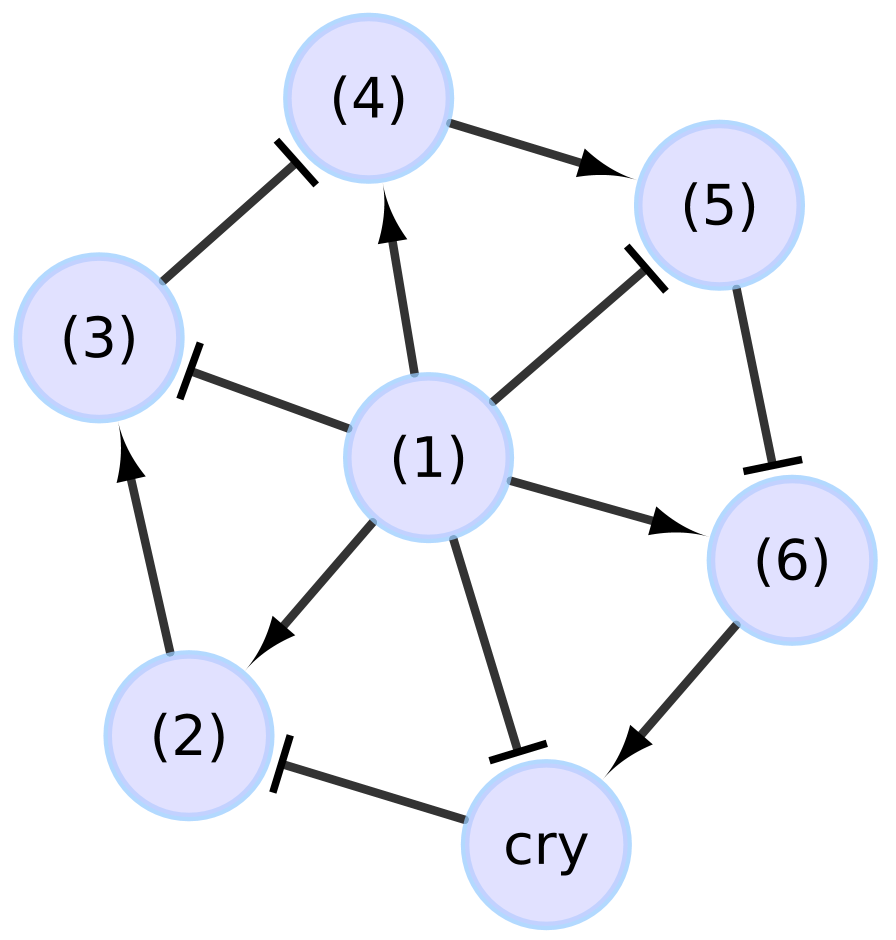
\includegraphics[scale=0.15]{images/drosophila_model_repressilator}}
\newlength\reprGraphHeight
\setlength\reprGraphHeight{\heightof{\reprGraph}}
\begin{figure}[!htb]
\begin{minipage}{\textwidth}
  \centering
  \subfloat[\label{subfig:repressilator-model}]{\begin{minipage}[c][\reprGraphHeight]{0.35\textwidth}\begin{center}\reprGraph\end{center}\end{minipage}}\qquad
  \subfloat[\label{subfig:repressilator-graph}]{\begin{minipage}[c][\reprGraphHeight]{0.6\textwidth}\begin{center}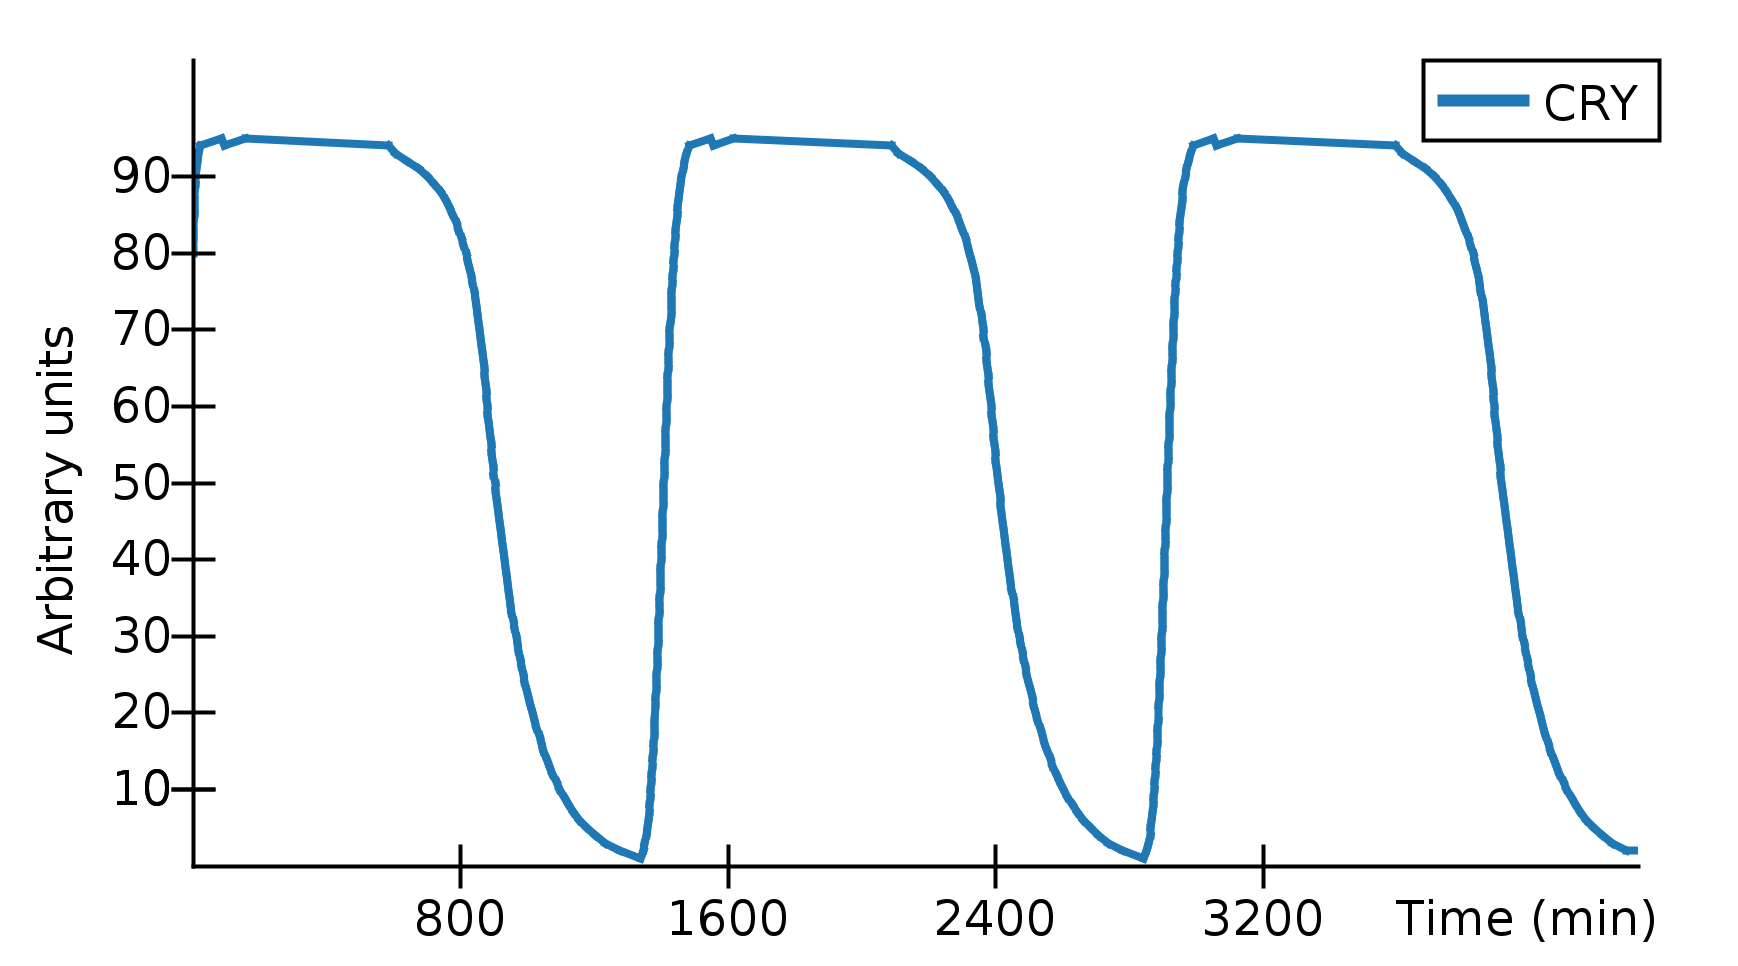
\includegraphics[width=\textwidth]{images/CRY_oscillations}\end{center}\end{minipage}}
\caption{{\bf \protect\subref{subfig:repressilator-model}} The repressilator-like subnetwork used to represent the alternation
between day and night that cause the oscillations in {\sf CRY} concentrations in the
network modelled in Section~\ref{sec:animo-drosophila}.
{\bf \protect\subref{subfig:repressilator-graph}} A graph plotting the oscillations in {\sf CRY} along
a period of three days.}\label{fig:repressilator}
\end{minipage}
\end{figure}


\subsection{ANIMO model of the Drosophila circadian clock}\label{suppl-sec:animo-drosophila}
Comparison between ODE and ANIMO models.
% The parameters of the ANIMO model used to represent the \emph{Drosophila Melanogaster} circadian clock in Section~\ref{sec:animo-drosophila}
% are given in Tables~\ref{tab:drosophila-model-reactants} and~\ref{tab:drosophila-model-reactions}.
% 
% 
% 
% \begin{table}[htbp]
% \begin{minipage}{\textwidth}
% \begin{center}
% \processtable{The settings for the nodes in the model from Section~\ref{sec:animo-drosophila}.\label{tab:drosophila-model-reactants}}
% % {\begin{tabular}{llllll}%|c|c|c|c|c|c|}
% % \ \\
% % \hline\noalign{\vskip 2mm}
% %   \multirow{2}{*}{{\bfseries Name}} & {\bfseries Total act.} & {\bfseries Initial act.} & \multirow{2}{*}{{\bfseries Molecule type}} &
% % \multirow{2}{*}{{\bfseries Enabled?}} & \multirow{2}{*}{{\bfseries Plotted?}}\\
% % & {\bfseries levels} & {\bfseries level} & & & \\[2mm]
% % \hline\noalign{\vskip 2mm}
% % clk & 100 & 98 & Other & Yes & Yes \\[5mm]
% % CLK & 100 & 100 & Other & Yes & Yes \\[5mm]
% % cry & 100 & 100 & Other & Yes & Yes \\[5mm]
% % CRY & 100 & 80 & Other & Yes & Yes \\[5mm]
% % cwo & 100 & 0 & Other & Yes & Yes \\[5mm]
% % CWO & 100 & 17 & Other & Yes & Yes \\[5mm]
% % CYC & 100 & 100 & Other & Yes & No \\[5mm]
% % CYC/CLK & 100 & 0 & Other & Yes & Yes \\[5mm]
% % DBT & 100 & 100 & Other & Yes & No \\[5mm]
% % pdp1 & 100 & 0 & Other & Yes & Yes \\[5mm]
% % PDP1 & 100 & 49 & Other & Yes & Yes \\[5mm]
% % PER & 100 & 5 & Other & Yes & Yes \\[5mm]
% % per & 100 & 0 & Other & Yes & Yes \\[5mm]
% % PER/TIM-p & 100 & 46 & Other & Yes & Yes \\[5mm]
% % tim & 100 & 0 & Other & Yes & Yes \\[5mm]
% % TIM & 100 & 5 & Other & Yes & Yes \\[5mm]
% % VRI & 100 & 39 & Other & Yes & Yes \\[5mm]
% % vri & 100 & 0 & Other & Yes & Yes \\[5mm]
% % (1) & 100 & 100 & Other & Yes & No \\[5mm]
% % (2) & 100 & 69 & Other & Yes & No \\[5mm]
% % (3) & 100 & 100 & Other & Yes & No \\[5mm]
% % (4) & 100 & 0 & Other & Yes & No \\[5mm]
% % (5) & 100 & 0 & Other & Yes & No \\[5mm]
% % (6) & 100 & 100 & Other & Yes & No \\[2mm]
% % \hline
% % \end{tabular}
% {\begin{tabular}{lll||lll}
% \ \\
% \hline%\noalign{\vskip 2mm}
% & & & & & \\[-1mm]
%   \multirow{2}{*}{{\bfseries Name}} & {\bfseries Total act.} & {\bfseries Initial act.} & \multirow{2}{*}{{\bfseries Name}} &
% {\bfseries Total act.} & {\bfseries Initial act.}\\
% & {\bfseries levels} & {\bfseries level} & & {\bfseries levels} & {\bfseries level} \\[2mm]
% \hline%\noalign{\vskip 5mm}
% & & & & & \\
% clk & 100 & 98 & per & 100 & 0 \\[5mm]
% CLK & 100 & 100 & PER/TIM-p & 100 & 46 \\[5mm]
% cry & 100 & 100 & tim & 100 & 0 \\[5mm]
% CRY & 100 & 80 & TIM & 100 & 5 \\[5mm]
% cwo & 100 & 0 & VRI & 100 & 39 \\[5mm]
% CWO & 100 & 17 & vri & 100 & 0 \\[5mm]
% CYC & 100 & 100 & (1) & 100 & 100 \\[5mm]
% CYC/CLK & 100 & 0 & (2) & 100 & 69 \\[5mm]
% DBT & 100 & 100 & (3) & 100 & 100 \\[5mm]
% pdp1 & 100 & 0 & (4) & 100 & 0 \\[5mm]
% PDP1 & 100 & 49 & (5) & 100 & 0 \\[5mm]
% PER & 100 & 5 & (6) & 100 & 100 \\[2mm]
% \hline
% \end{tabular}
% }{}
% \end{center}
% \end{minipage}
% \end{table}
% 
% 
% \begin{table}[!ht]
% \begin{minipage}{\textwidth}
% \processtable{The settings for the edges (interactions) in the model from Section~\ref{sec:animo-drosophila}.
% $\rightarrow$ indicates activation, while $\dashv$ stands for inhibition.\label{tab:drosophila-model-reactions}}
% {\begin{tabular}{lll||lll}
% \ \\
% \hline%\noalign{\vskip 2mm}
% & & & & & \\[-1mm]
%   {\bfseries Interaction} & {\bfseries Scenario} & {\bfseries Param. value} & {\bfseries Interaction} & {\bfseries Scenario} & {\bfseries Param. value}\\[2mm]
% \hline
% & & & \\
% % \noalign{\vskip 2mm}  DBT $\rightarrow$ PER/TIM-p & 1 & 0.001 & Activation\\[5mm]
% % \noalign{\vskip 2mm}  PER/TIM-p $\dashv$ CYC/CLK & 1 & 0.32 & Inhibition\\[5mm]
% % \noalign{\vskip 2mm}  CYC $\rightarrow$ CYC/CLK & 1 & 0.02 & Activation\\[5mm]
% % \noalign{\vskip 2mm}  CLK $\rightarrow$ CYC/CLK & 1 & 0.072 & Activation\\[5mm]
% % \noalign{\vskip 2mm}  clk $\rightarrow$ CLK & 1 & 0.024 & Activation\\[5mm]
% % \noalign{\vskip 2mm}  CYC/CLK $\rightarrow$ per & 1 & 0.031 & Activation\\[5mm]
% % \noalign{\vskip 2mm}  CYC/CLK $\rightarrow$ tim & 1 & 0.015 & Activation\\[5mm]
% % \noalign{\vskip 2mm}  CYC/CLK $\rightarrow$ cwo & 1 & 0.1 & Activation\\[5mm]
% % \noalign{\vskip 2mm}  CYC/CLK $\rightarrow$ pdp1 & 1 & 0.0375 & Activation\\[5mm]
% % \noalign{\vskip 2mm}  CYC/CLK $\rightarrow$ vri & 1 & 0.03 & Activation\\[5mm]
% % \noalign{\vskip 2mm}  TIM $\rightarrow$ PER/TIM-p & 1 & 0.069 & Activation\\[5mm]
% % \noalign{\vskip 2mm}  PER $\rightarrow$ PER/TIM-p & 1 & 0.053 & Activation\\[5mm]
% % \noalign{\vskip 2mm}  per $\rightarrow$ PER & 1 & 0.0075 & Activation\\[5mm]
% % \noalign{\vskip 2mm}  cwo $\rightarrow$ CWO & 1 & 0.03 & Activation\\[5mm]
% % \noalign{\vskip 2mm}  CWO $\dashv$ cwo & 1 & 0.112 & Inhibition\\[5mm]
% % \noalign{\vskip 2mm}  vri $\rightarrow$ VRI & 1 & 0.026 & Activation\\[5mm]
% % \noalign{\vskip 2mm}  VRI $\dashv$ clk & 1 & 0.0098 & Inhibition\\[5mm]
% % \noalign{\vskip 2mm}  CWO $\dashv$ per & 1 & 0.05 & Inhibition\\[5mm]
% % \noalign{\vskip 2mm}  CWO $\dashv$ vri & 1 & 0.024 & Inhibition\\[5mm]
% % \noalign{\vskip 2mm}  CWO $\dashv$ tim & 1 & 0.02 & Inhibition\\[5mm]
% % \noalign{\vskip 2mm}  CWO $\dashv$ pdp1 & 1 & 0.0384 & Inhibition\\[5mm]
% % \noalign{\vskip 2mm}  tim $\rightarrow$ TIM & 1 & 0.056 & Activation\\[5mm]
% % \noalign{\vskip 2mm}  pdp1 $\rightarrow$ PDP1 & 1 & 0.042 & Activation\\[5mm]
% % \noalign{\vskip 2mm}  PDP1 $\rightarrow$ clk & 1 & 0.01 & Activation\\[5mm]
% % \noalign{\vskip 2mm}  cry $\rightarrow$ CRY & 2 & 0.9733 & Activation\\[5mm]
% % \noalign{\vskip 2mm}  CRY $\dashv$ TIM & 1 & 0.048 & Inhibition\\[5mm]
% % \noalign{\vskip 2mm}  cry $\dashv$ (2) & 1 & 0.10512 & Inhibition\\[5mm]
% % \noalign{\vskip 2mm}  (2) $\rightarrow$ (3) & 1 & 0.10512 & Activation\\[5mm]
% % \noalign{\vskip 2mm}  (3) $\dashv$ (4) & 1 & 0.10512 & Inhibition\\[5mm]
% % \noalign{\vskip 2mm}  (4) $\rightarrow$ (5) & 1 & 0.10512 & Activation\\[5mm]
% % \noalign{\vskip 2mm}  (5) $\dashv$ (6) & 1 & 0.10512 & Inhibition\\[5mm]
% % \noalign{\vskip 2mm}  (6) $\rightarrow$ cry & 1 & 0.10512 & Activation\\[5mm]
% % \noalign{\vskip 2mm}  (1) $\dashv$ cry & 1 & 0.0257 & Inhibition\\[5mm]
% % \noalign{\vskip 2mm}  (1) $\rightarrow$ (2) & 1 & 0.0.0518 & Activation\\[5mm]
% % \noalign{\vskip 2mm}  (1) $\dashv$ (3) & 1 & 0.0257 & Inhibition\\[5mm]
% % \noalign{\vskip 2mm}  (1) $\rightarrow$ (4) & 1 & 0.0518 & Activation\\[5mm]
% % \noalign{\vskip 2mm}  (1) $\dashv$ (5) & 1 & 0.0257 & Inhibition\\[5mm]
% % \noalign{\vskip 2mm}  (1) $\rightarrow$ (6) & 1 & 0.0518 & Activation\\[2mm]
% DBT $\rightarrow$ PER/TIM-p & 1 & 0.001 & CWO $\dashv$ tim & 1 & 0.02 \\[5mm]
% PER/TIM-p $\dashv$ CYC/CLK & 1 & 0.32 & CWO $\dashv$ pdp1 & 1 & 0.0384 \\[5mm]
% CYC $\rightarrow$ CYC/CLK & 1 & 0.02 & tim $\rightarrow$ TIM & 1 & 0.056 \\[5mm]
% CLK $\rightarrow$ CYC/CLK & 1 & 0.072 & pdp1 $\rightarrow$ PDP1 & 1 & 0.042 \\[5mm]
% clk $\rightarrow$ CLK & 1 & 0.024 & PDP1 $\rightarrow$ clk & 1 & 0.01 \\[5mm]
% CYC/CLK $\rightarrow$ per & 1 & 0.031 & cry $\rightarrow$ CRY & 2 & 0.9733 \\[5mm]
% CYC/CLK $\rightarrow$ tim & 1 & 0.015 & CRY $\dashv$ TIM & 1 & 0.048 \\[5mm]
% CYC/CLK $\rightarrow$ cwo & 1 & 0.1 & cry $\dashv$ (2) & 1 & 0.10512 \\[5mm]
% CYC/CLK $\rightarrow$ pdp1 & 1 & 0.0375 & (2) $\rightarrow$ (3) & 1 & 0.10512 \\[5mm]
% CYC/CLK $\rightarrow$ vri & 1 & 0.03 & (3) $\dashv$ (4) & 1 & 0.10512 \\[5mm]
% TIM $\rightarrow$ PER/TIM-p & 1 & 0.069 & (4) $\rightarrow$ (5) & 1 & 0.10512 \\[5mm]
% PER $\rightarrow$ PER/TIM-p & 1 & 0.053 & (5) $\dashv$ (6) & 1 & 0.10512 \\[5mm]
% per $\rightarrow$ PER & 1 & 0.0075 & (6) $\rightarrow$ cry & 1 & 0.10512 \\[5mm]
% cwo $\rightarrow$ CWO & 1 & 0.03 & (1) $\dashv$ cry & 1 & 0.0257 \\[5mm]
% CWO $\dashv$ cwo & 1 & 0.112 & (1) $\rightarrow$ (2) & 1 & 0.0.0518 \\[5mm]
% vri $\rightarrow$ VRI & 1 & 0.026 & (1) $\dashv$ (3) & 1 & 0.0257 \\[5mm]
% VRI $\dashv$ clk & 1 & 0.0098 & (1) $\rightarrow$ (4) & 1 & 0.0518 \\[5mm]
% CWO $\dashv$ per & 1 & 0.05 & (1) $\dashv$ (5) & 1 & 0.0257 \\[5mm]
% CWO $\dashv$ vri & 1 & 0.024 & (1) $\rightarrow$ (6) & 1 & 0.0518 \\[2mm]
% \hline
% \end{tabular}}{}
% \end{minipage}
% \end{table}\vspace{-2ex}


\subsection{Note on the parameters in the TNF$\alpha$-EGF model}\label{suppl:parameters-tnf-egf}
The parameters in the model in Figure~\ref{fig:large-model-complete}
have been set by fitting the model to the experimental data for conditions with 100 ng/ml TNF$\alpha$.
In the model we have set the starting level of TNF$\alpha$ at 100 out of 100 for these conditions.
This level is a dimensionless quantity that indicates the maximum activity level in the data set.
We found that setting the initial level of TNF$\alpha$ at level 8 out of 100 gave slightly better results for the
condition with 5 ng/ml TNF$\alpha$ than level 5 out of 100. We believe that this has to do with the fact that
100 ng/ml is a highly supra-physiological concentration of TNF$\alpha$, that will rapidly cause activation of all
receptors present. Fitting the model to this experimental condition may have resulted in slight deviations
in the parameter values. Nevertheless, the modelling results illustrate that building a model with basic
kinetic rate laws can give useful predictions over a range of concentrations. Figures~\ref{fig:large-model-graph3} and~\ref{fig:large-model-graph4}
show the modelling results with TNF set at 8 out of 100.


\clearpage
\section{Comparison between ANIMO and other modelling tools}\label{suppl:comparison-table}
Different formalisms are in use in the field of computational
modelling of biological systems, each with their specific characteristics.
Many of these formalisms have been implemented into
software tools to support modelling efforts. In order to compare
ANIMO with existing tools, we have selected a number of mathematical formalisms,
each connected to a supporting tool. With an emphasis on the modelling
process rather than the final model, we compared these tools on
the basis of the following parameters:

\begin{enumerate}
  \item {\bf Hidden formalism:} a knowledge of the underlying formalism is not required in order to use the tool
  \item {\bf Visual modelling:} the tool allows the user to model using a visual interface, and is not exclusively
      founded on formula-, text- or table-based input forms
  \item {\bf Qualitative parameters:} parameters for reactions can be input as approximated estimations, and not exclusively as numbers
  \item {\bf Tight coupling with topology:} models are tightly and clearly coupled to the networks they represent, showing the visual
      representation of the model in a shape similar or comparable to the representation currently used by biologists
      for signalling pathways
  \item {\bf User-chosen granularity:} if discretization is applied during the modelling process, the user can change the granularity
      with which such discretization is made, possibly for each component of the model separately
\end{enumerate}
Table~\ref{tab:tool-comparison} shows the comparison between ANIMO and the selected tools.

\newcolumntype{x}[1]{%
>{\centering\hspace{0pt}}p{#1}}%
\savenotes
\begin{table}[!hbt]
\begin{minipage}{\textwidth}
\processtable{Comparison between ANIMO and some existing approaches to modelling biological systems.
A ``Yes'' under a column indicates that the modelling tool (mostly) fulfils the parameter, ``No'' indicates very limited or no fulfilment.
\label{tab:tool-comparison}}
{\begin{tabular}{p{4cm}p{1.8cm}p{1.8cm}p{1.5cm}p{1.8cm}p{1.8cm}p{2cm}}
\toprule
{\bfseries Tool} & {\bfseries Formalism} & {\bfseries Hidden formalism} & {\bfseries Visual modelling} & {\bfseries Qualitative parameters} & {\bfseries Tight coupling with topology} & {\bfseries User-chosen granularity}  \\[5mm]
\midrule
\noalign{\vskip 2mm} ANIMO~\citep{animo-bibe} & Timed \ \ \ Automata & Yes & Yes & Yes & Yes & Yes
      \\[5mm]
\noalign{\vskip 2mm} Bio-PEPA Workbench~\citep{biopepa-interface} & Bio-PEPA & No & No & No & No & Yes
      \\[5mm]
\noalign{\vskip 2mm} Cell Illustrator~\citep{cell-illustrator} & Petri Nets & Yes & Yes & No & Yes & No
     \\[5mm]
\noalign{\vskip 2mm} COPASI~\citep{copasi} & ODE, stochastic models & No & No & No & No & No
      \\[5mm]
\noalign{\vskip 2mm} COSBI LAB~$^1$
 & BlenX & Yes & Yes & No & Yes & No
      \\[5mm]
\noalign{\vskip 2mm} GINsim~\citep{ginsim} & Boolean Networks & No & Yes & Yes & Yes & Yes~$^2$
      \\[5mm]
\noalign{\vskip 2mm} GNA~\citep{gna}    & ODE & No & Yes & Yes & Yes & No~$^3$
      \\
\noalign{\vskip 2mm} Rhapsody~$^4$
 & Statecharts & No & Yes & Yes & No~$^5$ & No
      \\[5mm]
\botrule
\end{tabular}}{$^1$ {COSBILab} web page \url{http://www.cosbi.eu/index.php/research/cosbi-lab}\\
$^2$ The user can choose the number of levels for each reactant, allowing to define
multi-level models based on Boolean reaction dynamics.\\
$^3$ When discretizing an ODE model, the granularity depends on the mathematical
features of the model, and not directly on the user's choice.\\
$^4$ {IBM Rational Rhapsody} web page \url{http://www-01.ibm.com/software/rational/products/rhapsody/designer}\\
$^5$ Statecharts represent more closely the so-called
\emph{transition system} of the model as opposed to the components and interactions occurring among them.}
\end{minipage}
\end{table}



% \addcontentsline{toc}{section}{References}
% \begin{thebibliography}{}
% ...
% \end{thebibliography}




\clearpage

\section{Supplementary figures}\label{sec:supplementary-figures}


\begin{figure}[htpb]
\begin{minipage}{\textwidth}
\centering
  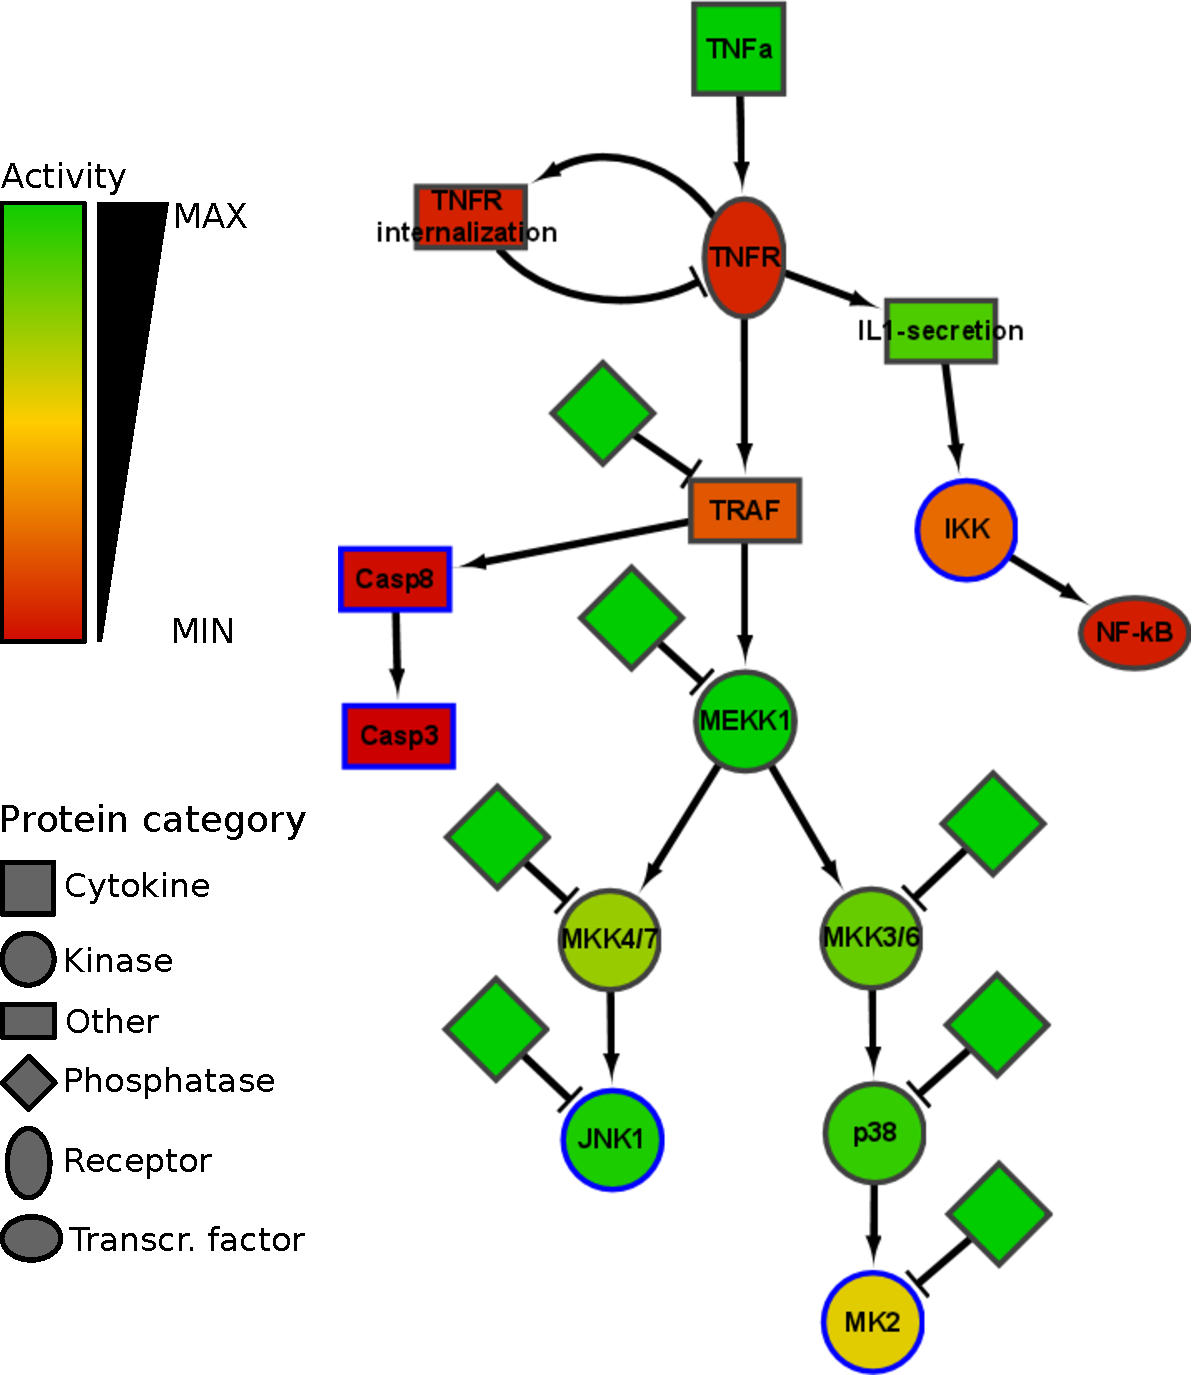
\includegraphics[width=.7\textwidth]{images/large_network_tnfa2}
\caption{The model for the TNF$\alpha$ pathway in isolation. Node colours represent the activity level of the
corresponding modelled reactants at time $t = 10$ minutes after a stimulation of 100 ng/ml TNF$\alpha$.}\label{fig:large-model-tnf}
\end{minipage}
\end{figure}

\begin{figure}[!tpb]
\begin{minipage}{\textwidth}
\centering
  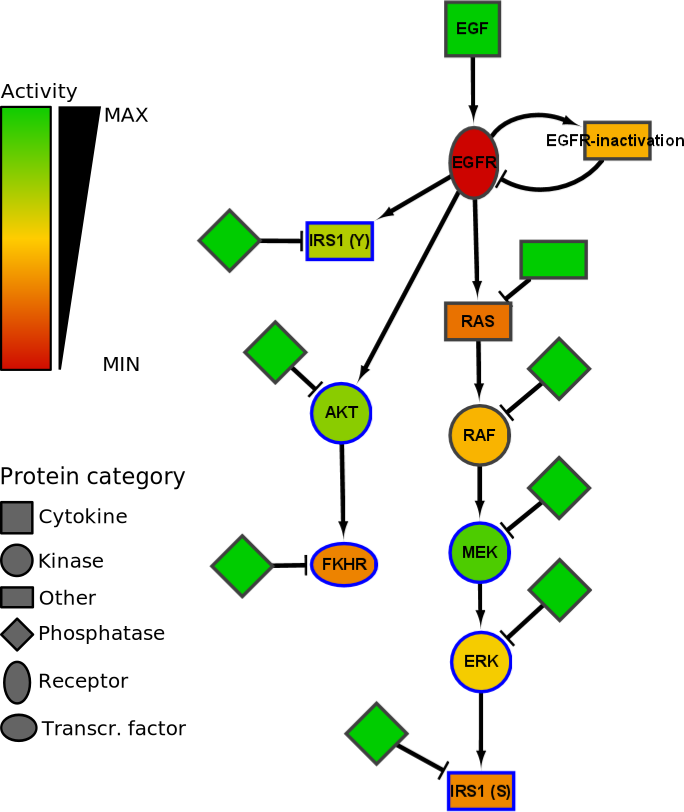
\includegraphics[width=.7\textwidth]{images/large_network_egf3}
\caption{The model for the EGF pathway in isolation. Node colours represent the
activity level of the corresponding modelled reactants at time $t = 5$ minutes after
a stimulation of 100 ng/ml EGF.}\label{fig:large-model-egf}
\end{minipage}
\end{figure}


\begin{figure}[!tpb]
\begin{minipage}{\textwidth}
\centering
  \subfloat{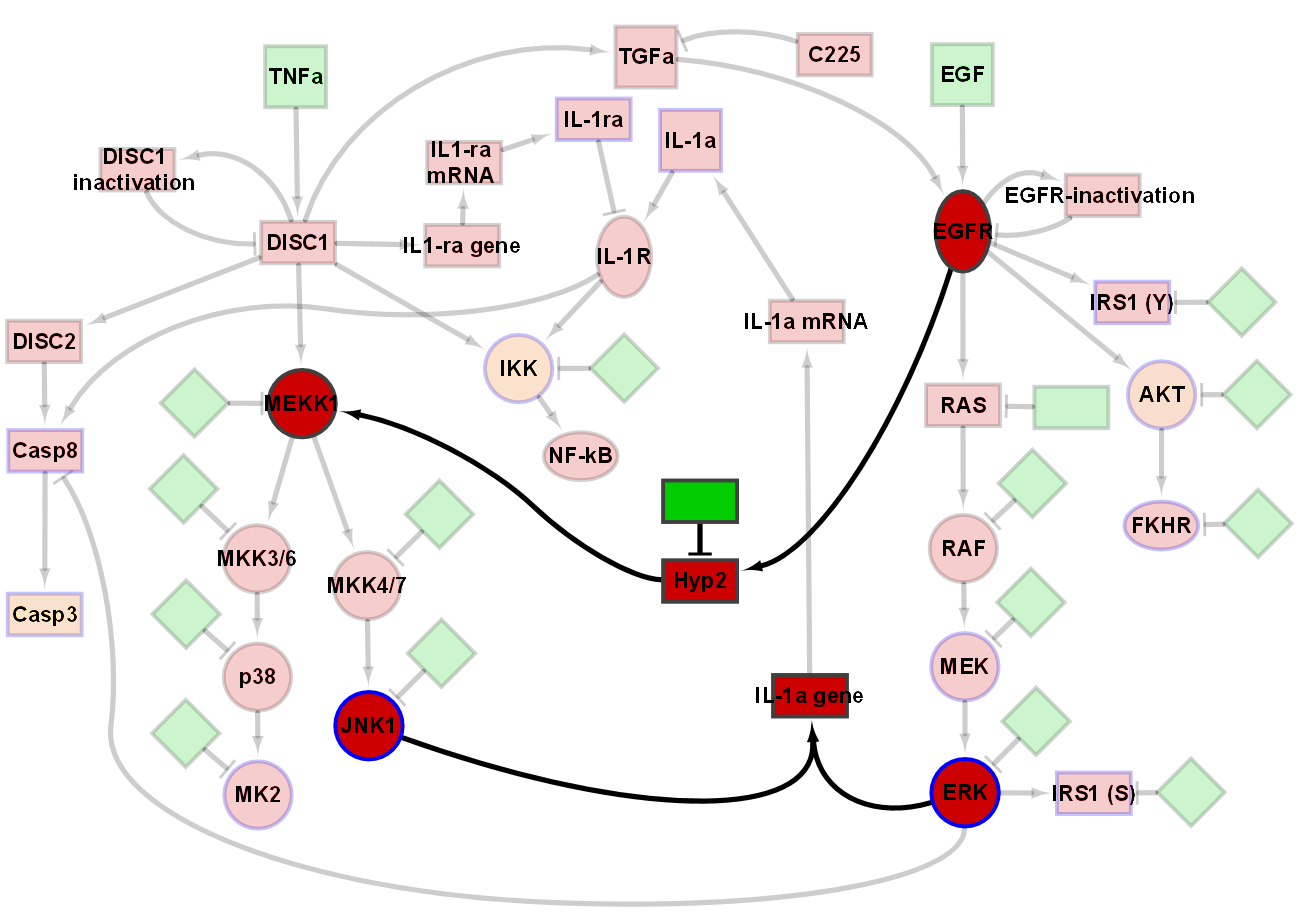
\includegraphics[width=\textwidth]{images/large_network_hypotheses7}}\\
\subfloat{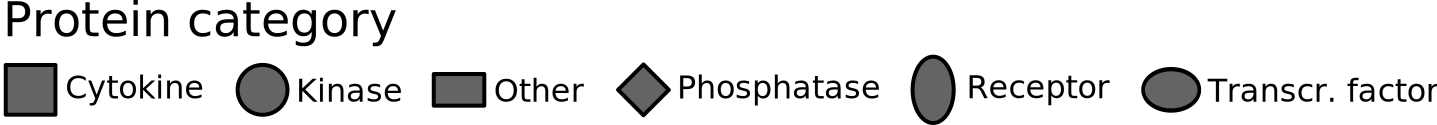
\includegraphics[scale=\legendScalaColori]{images/legenda_forme}} \subfloat{
\includegraphics[scale=\legendScalaForme]{images/legenda_colori}}
\caption{The merged model for the TNF$\alpha$-EGF pathway in which 
the two hypotheses are highlighted. The first hypothesis is the dependence IL-1$\alpha$ expression on the 
combined activity of ERK and JNK1. The second hypothesis assumes an as yet unidentified protein (Hyp2) to link EGFR to MEKK1.
Node colours represent initial activity levels.}\label{fig:large-model-hypotheses}
\end{minipage}
\end{figure}


\renewcommand*\thesubfigure{}
\begin{figure}[!tpb]
\begin{minipage}{\textwidth}
\begin{tabularx}{\textwidth}{XXX}
\subfloat[MK2 (2 hours)]{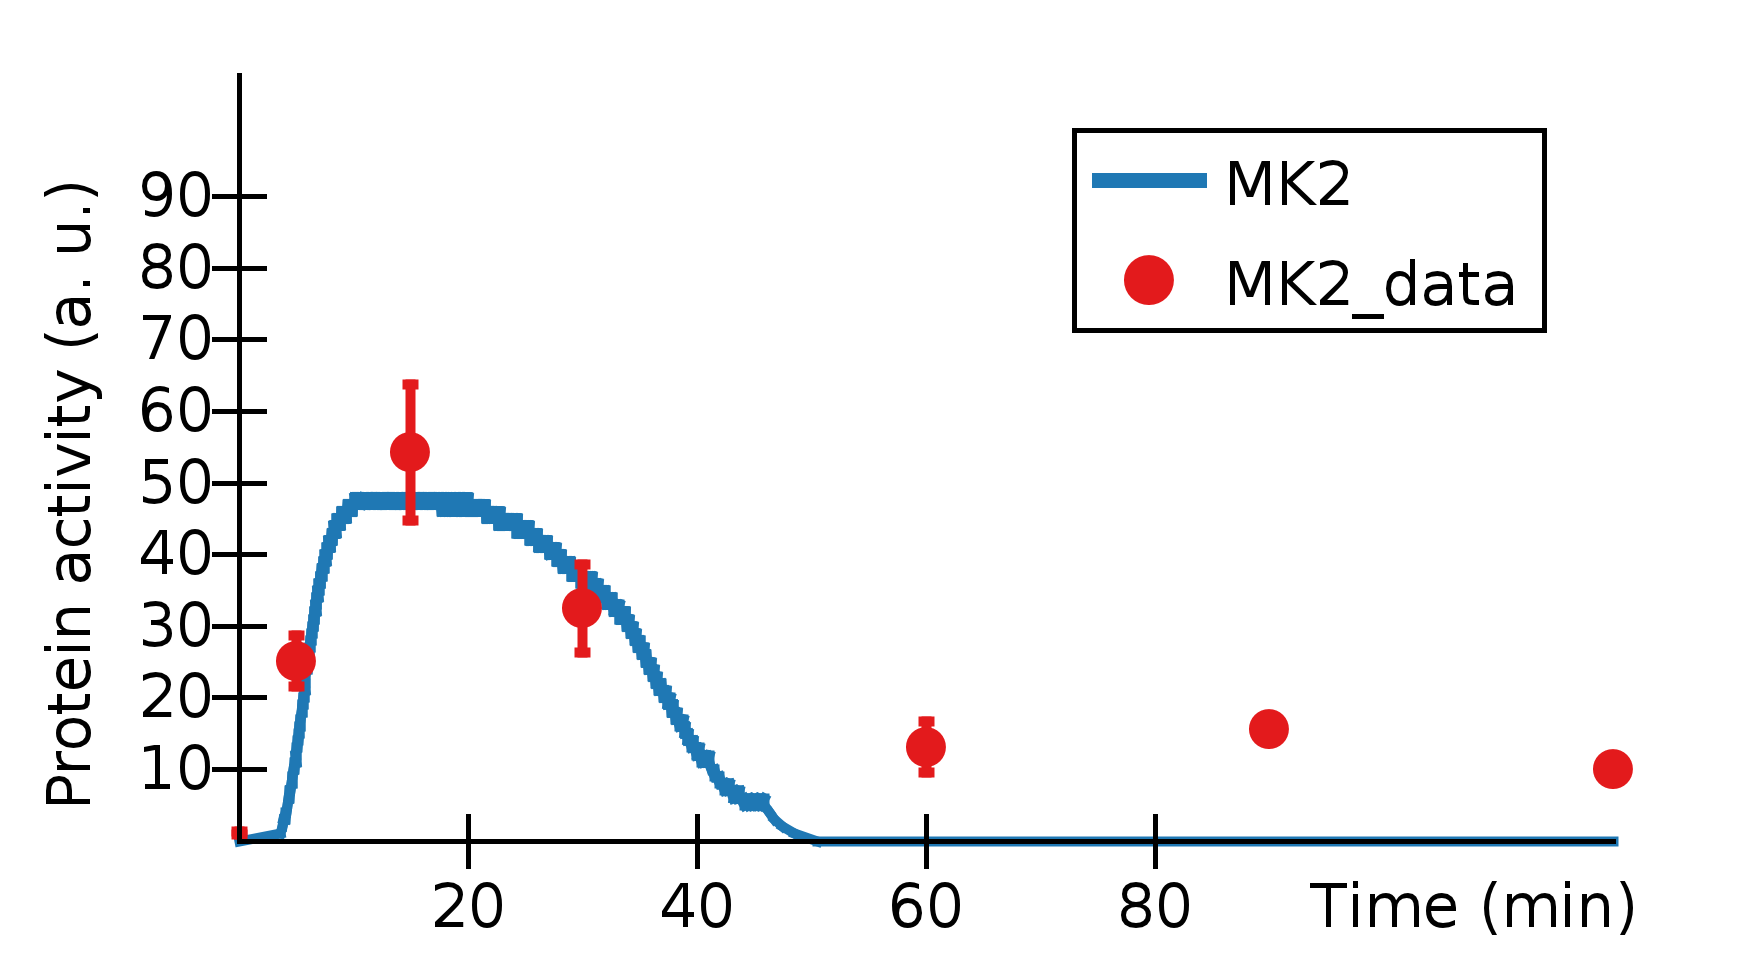
\includegraphics[width=0.29\textwidth]{images/TNFa100/MK2}} &
\subfloat[JNK1 (2 hours)]{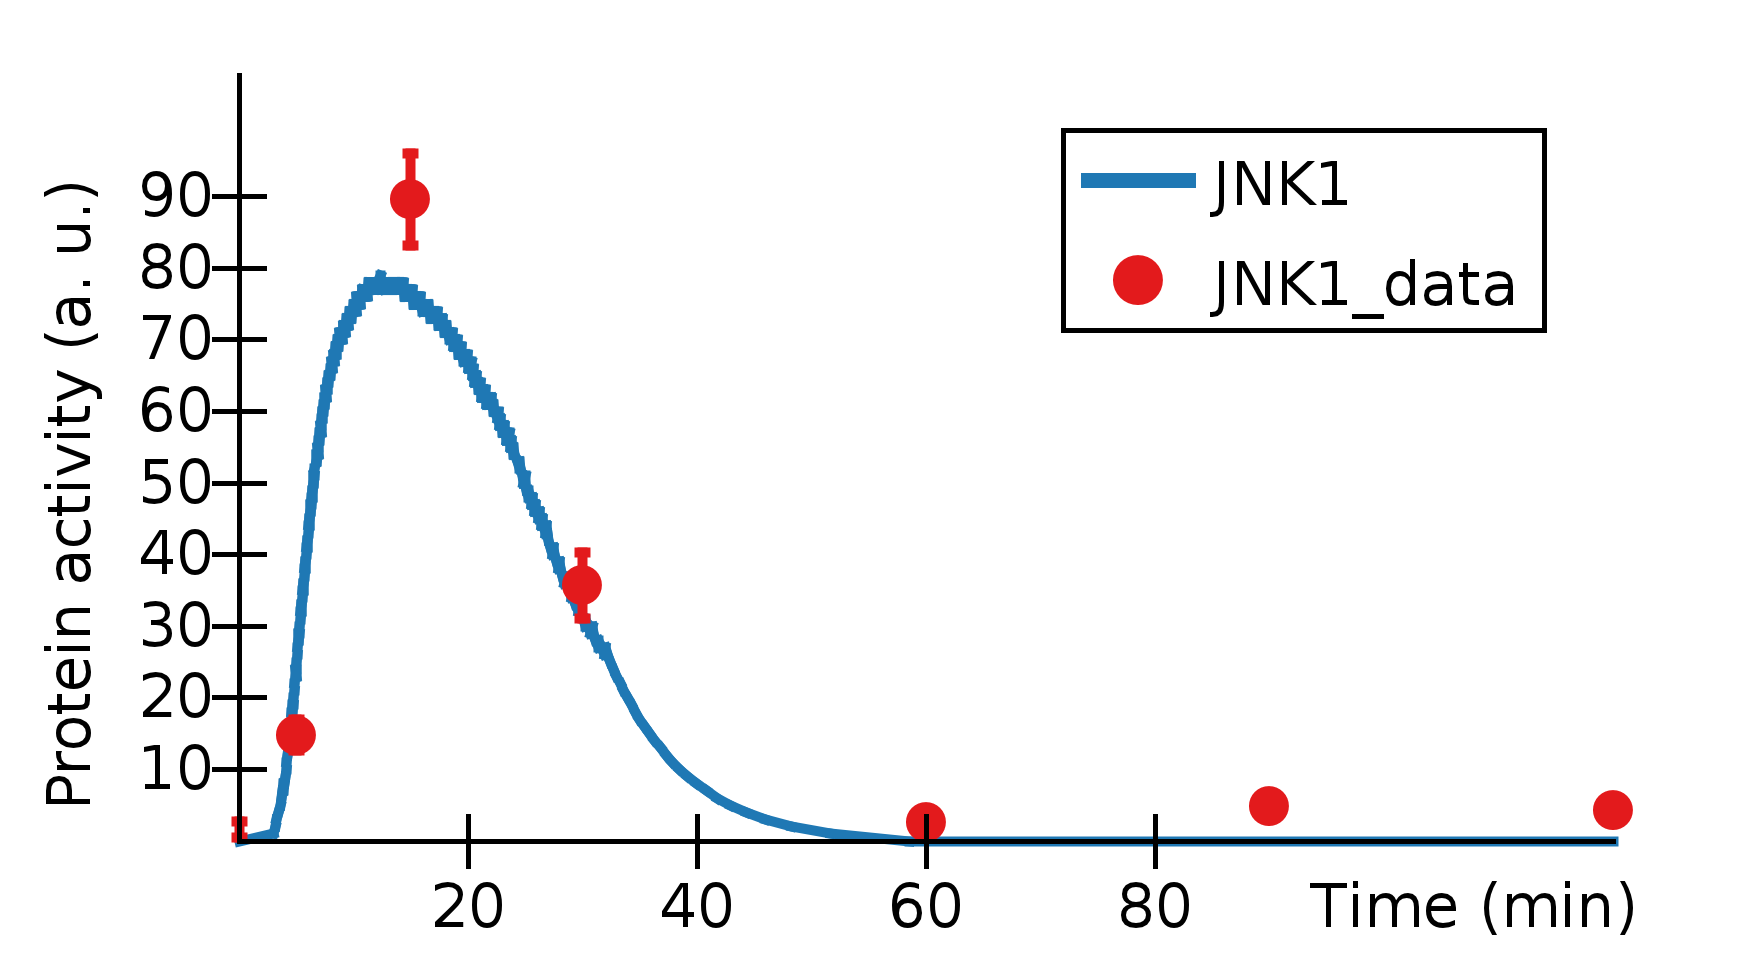
\includegraphics[width=0.29\textwidth]{images/TNFa100/JNK1}} &
\subfloat[IKK (2 hours)]{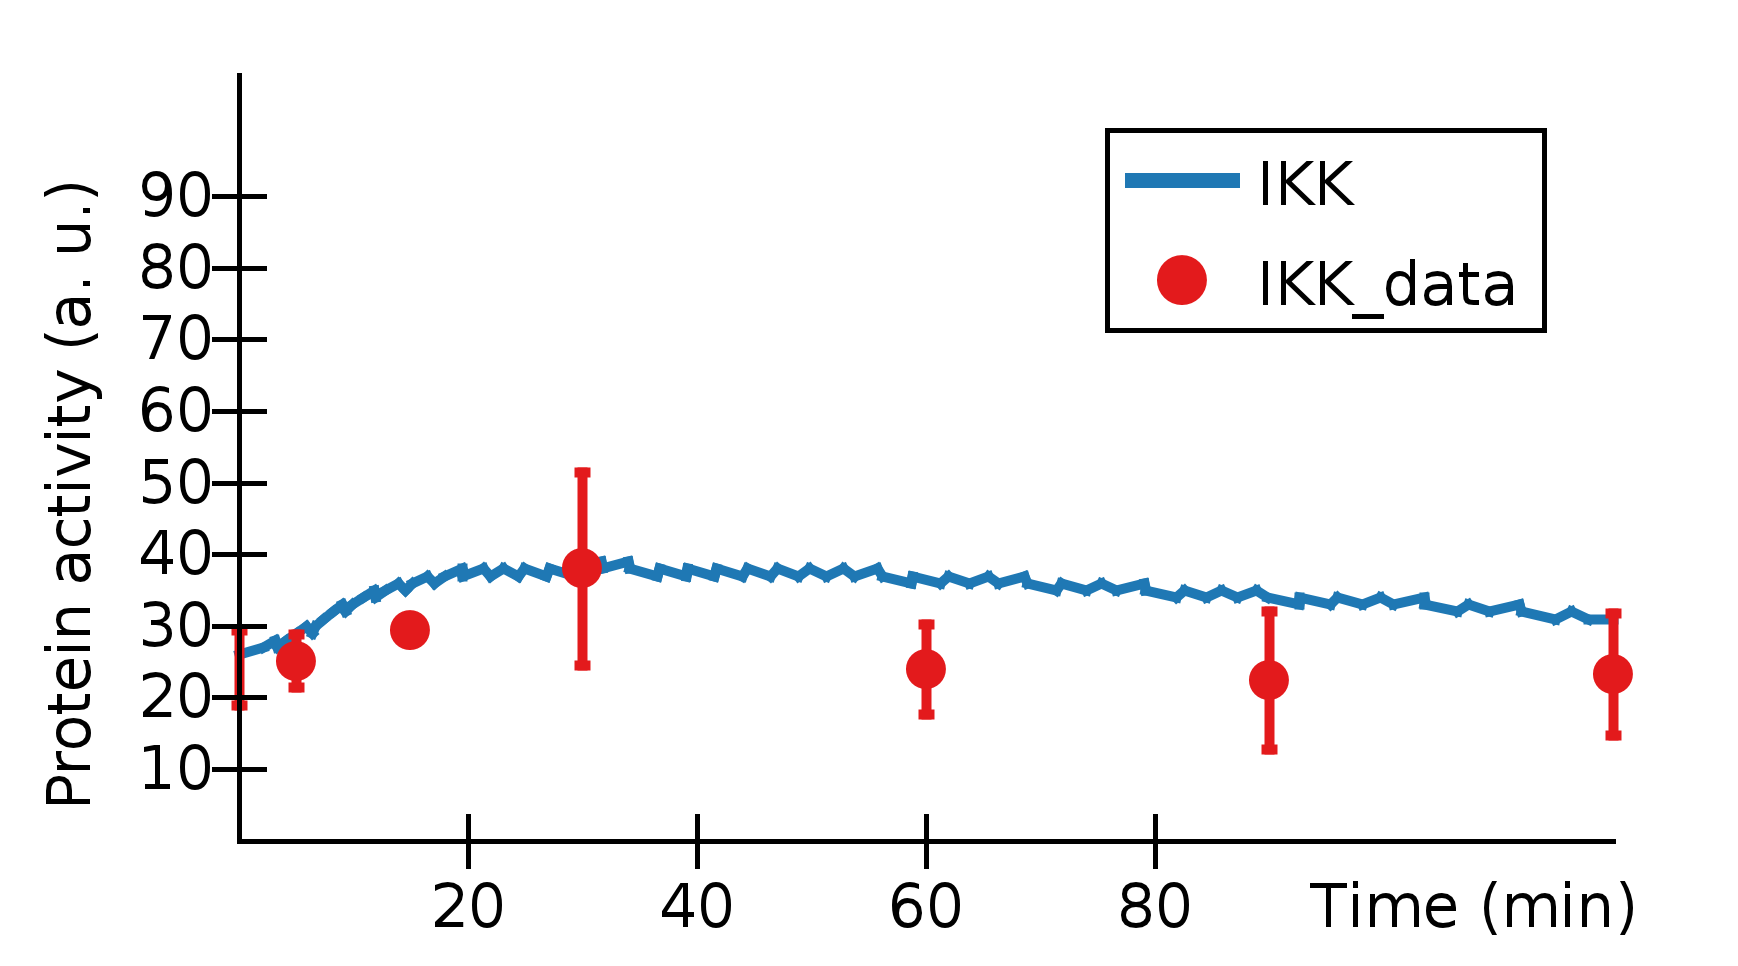
\includegraphics[width=0.29\textwidth]{images/TNFa100/IKK_120}} \\
\subfloat[IKK (24 hours)]{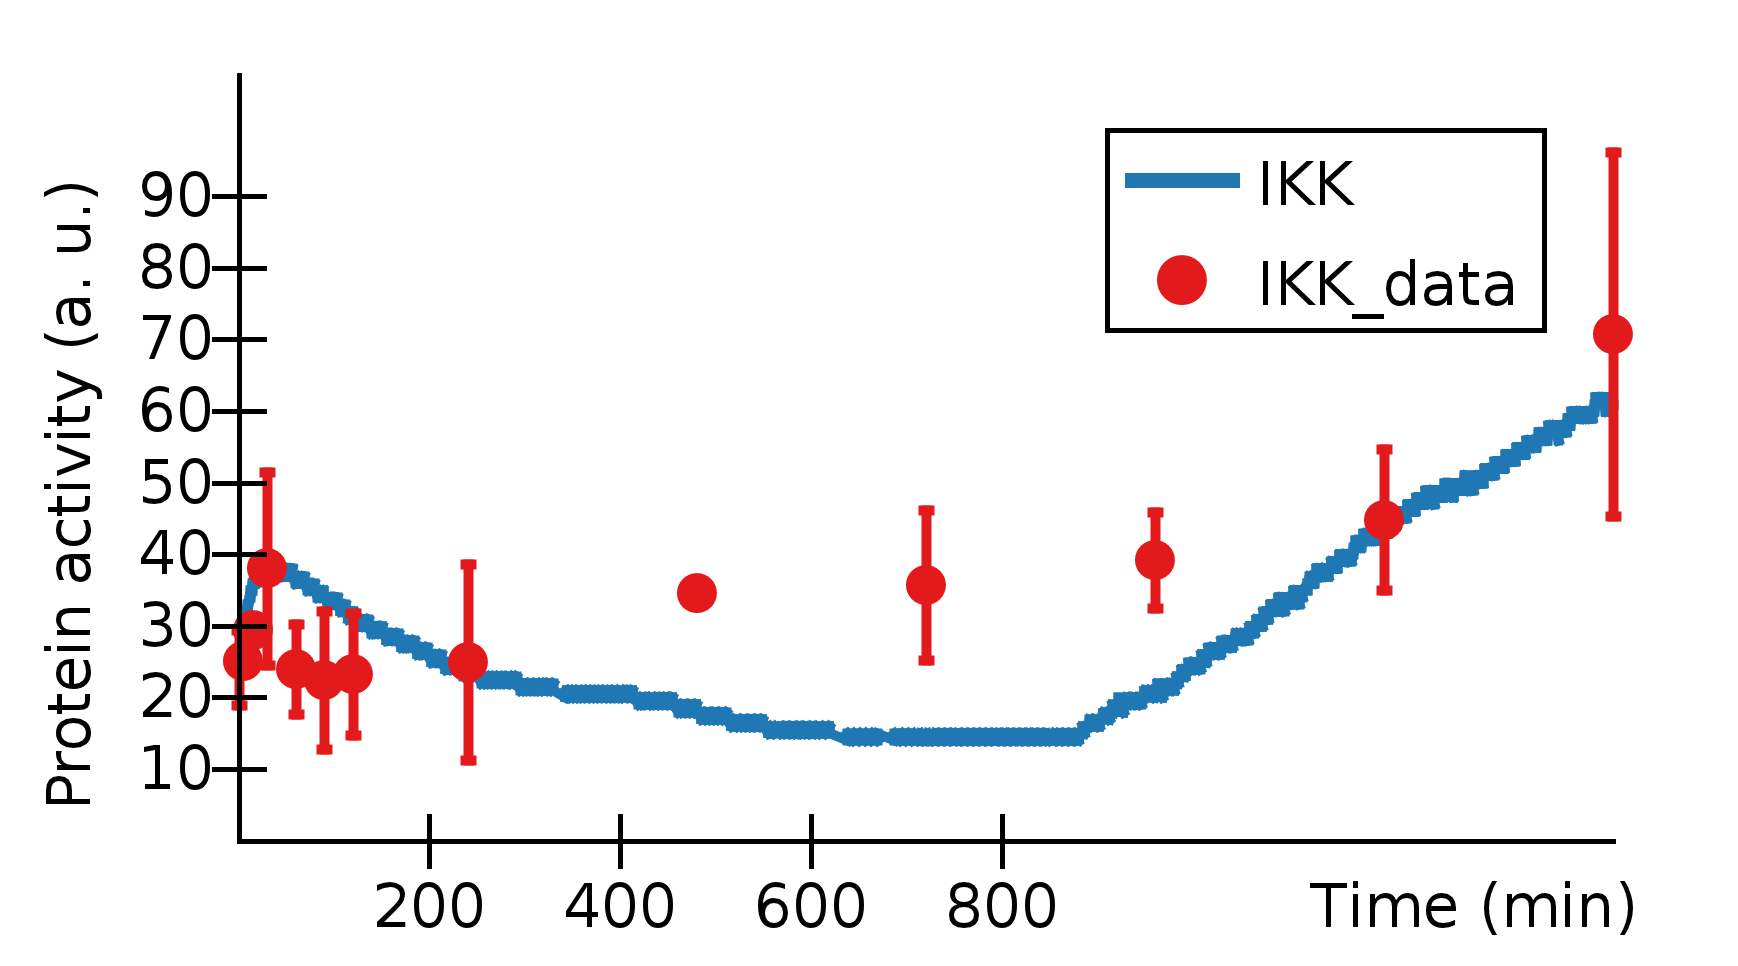
\includegraphics[width=0.29\textwidth]{images/TNFa100/IKK_1440}} &
\subfloat[caspase-8 (24 hours)]{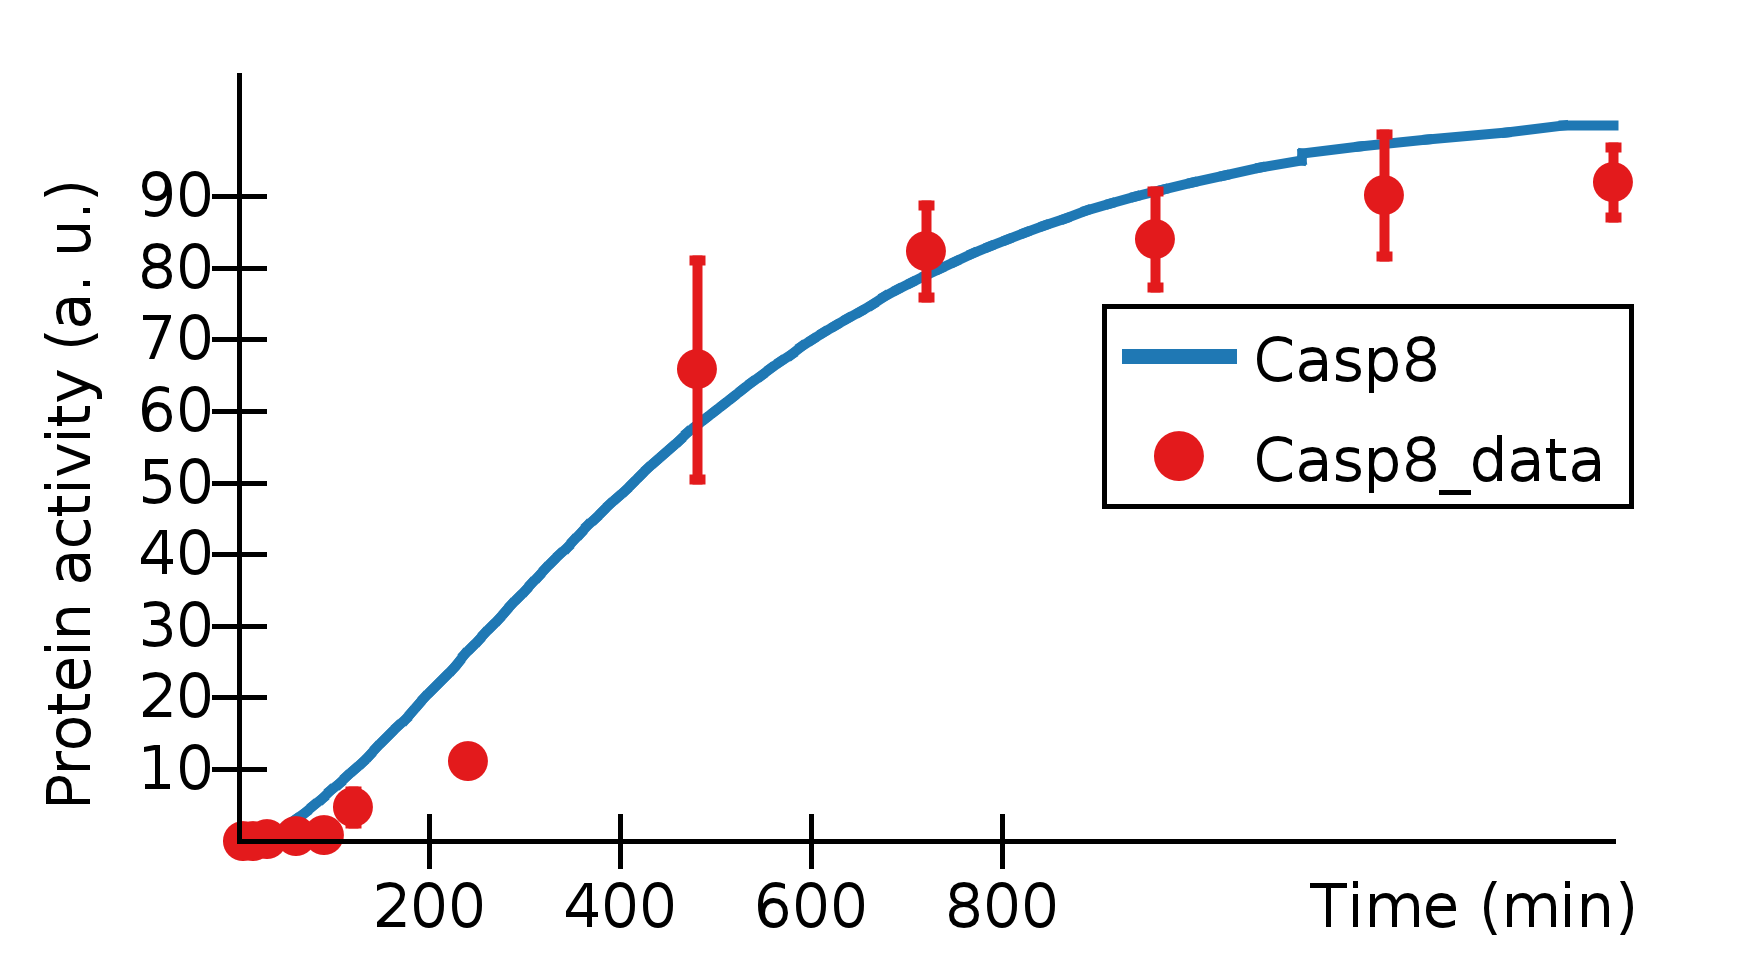
\includegraphics[width=0.29\textwidth]{images/TNFa100/casp8}} &
\subfloat[caspase-3 (24 hours)]{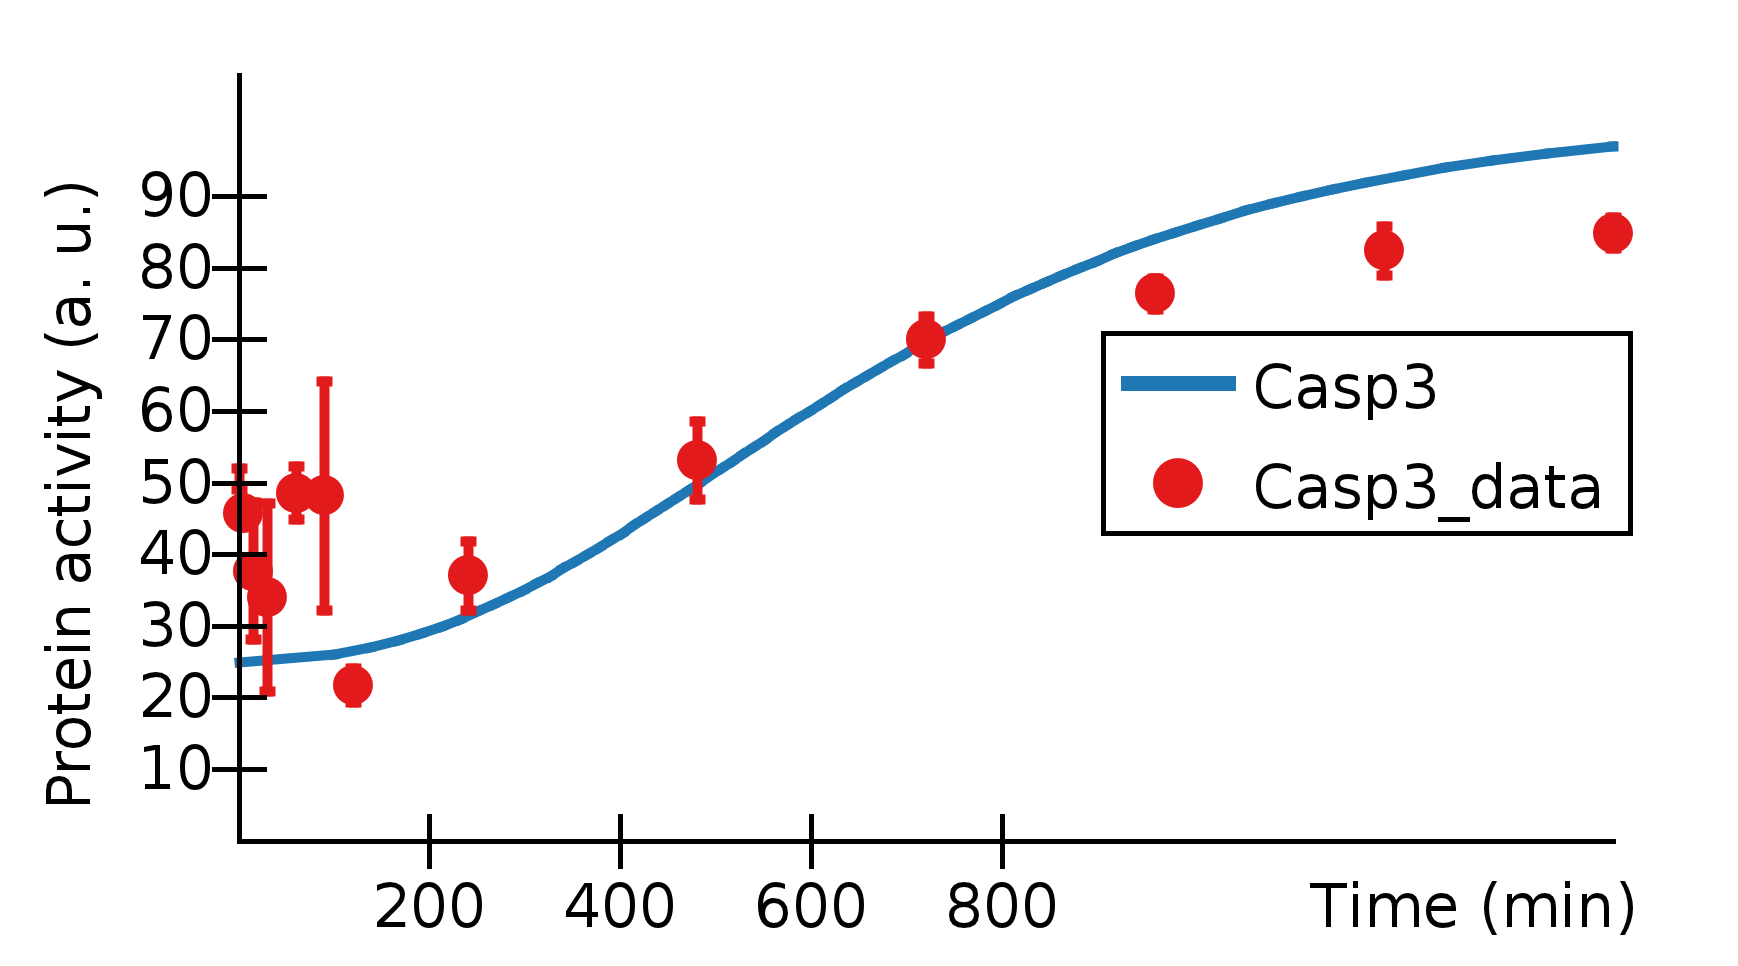
\includegraphics[width=0.29\textwidth]{images/TNFa100/casp3}} \\
\subfloat[MEK (2 hours)]{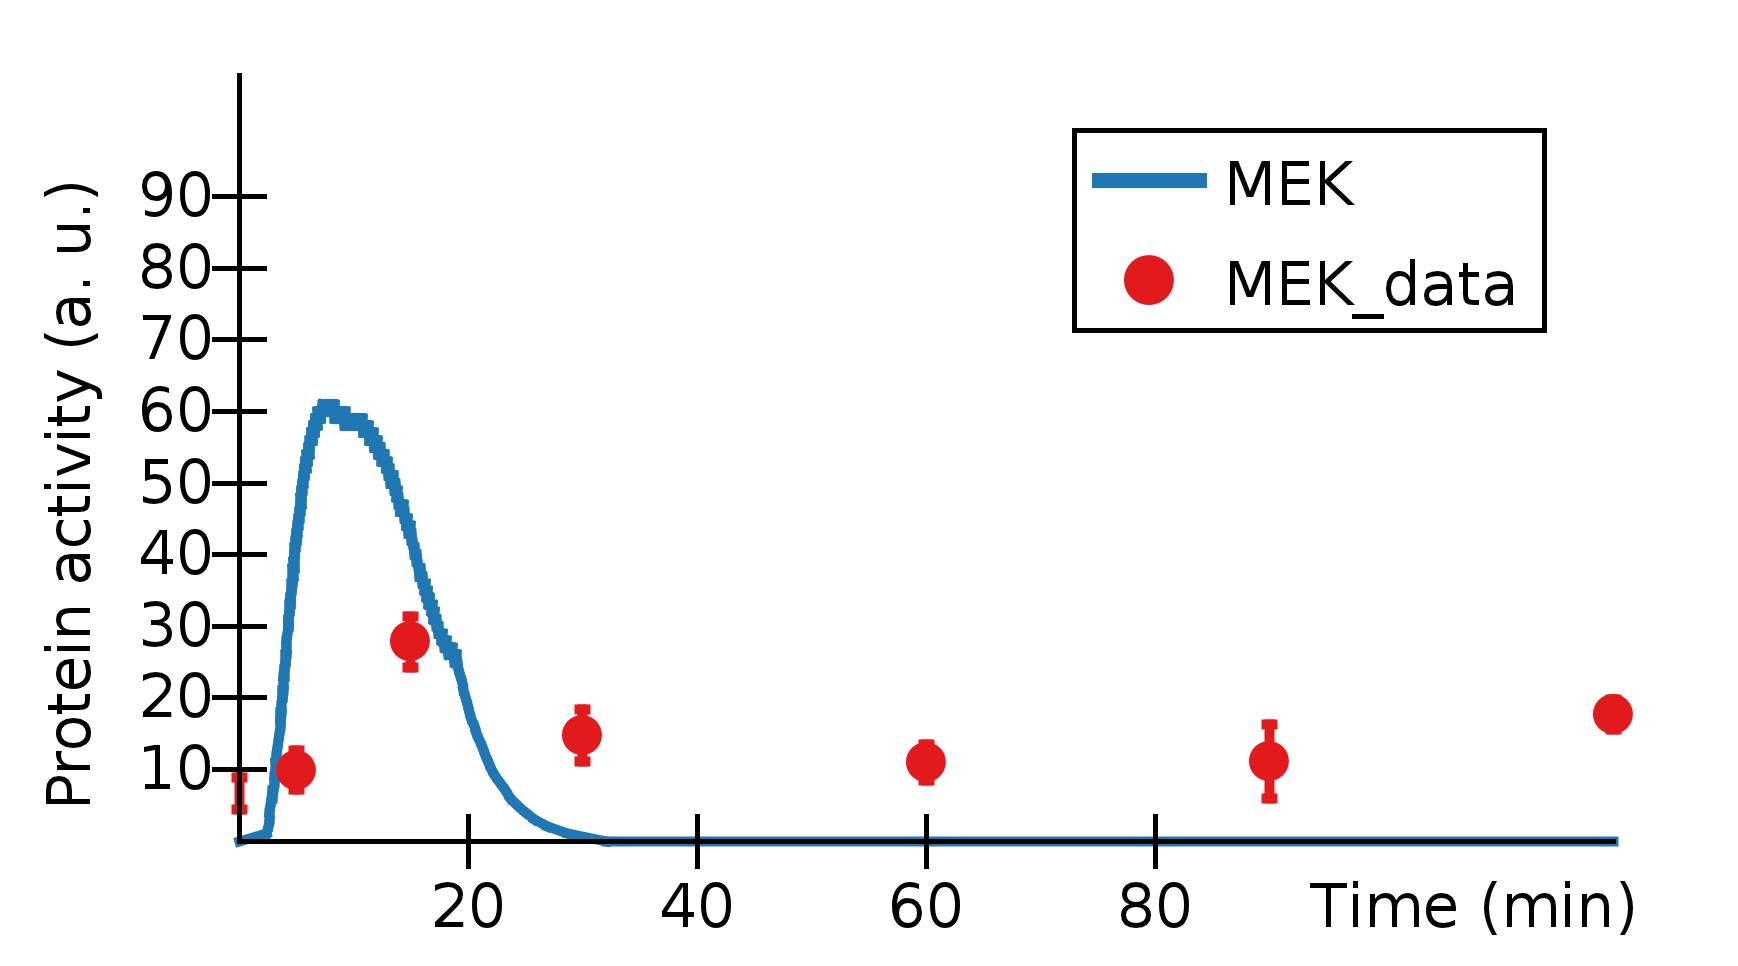
\includegraphics[width=0.29\textwidth]{images/TNFa100/MEK}} &
\subfloat[ERK (2 hours)]{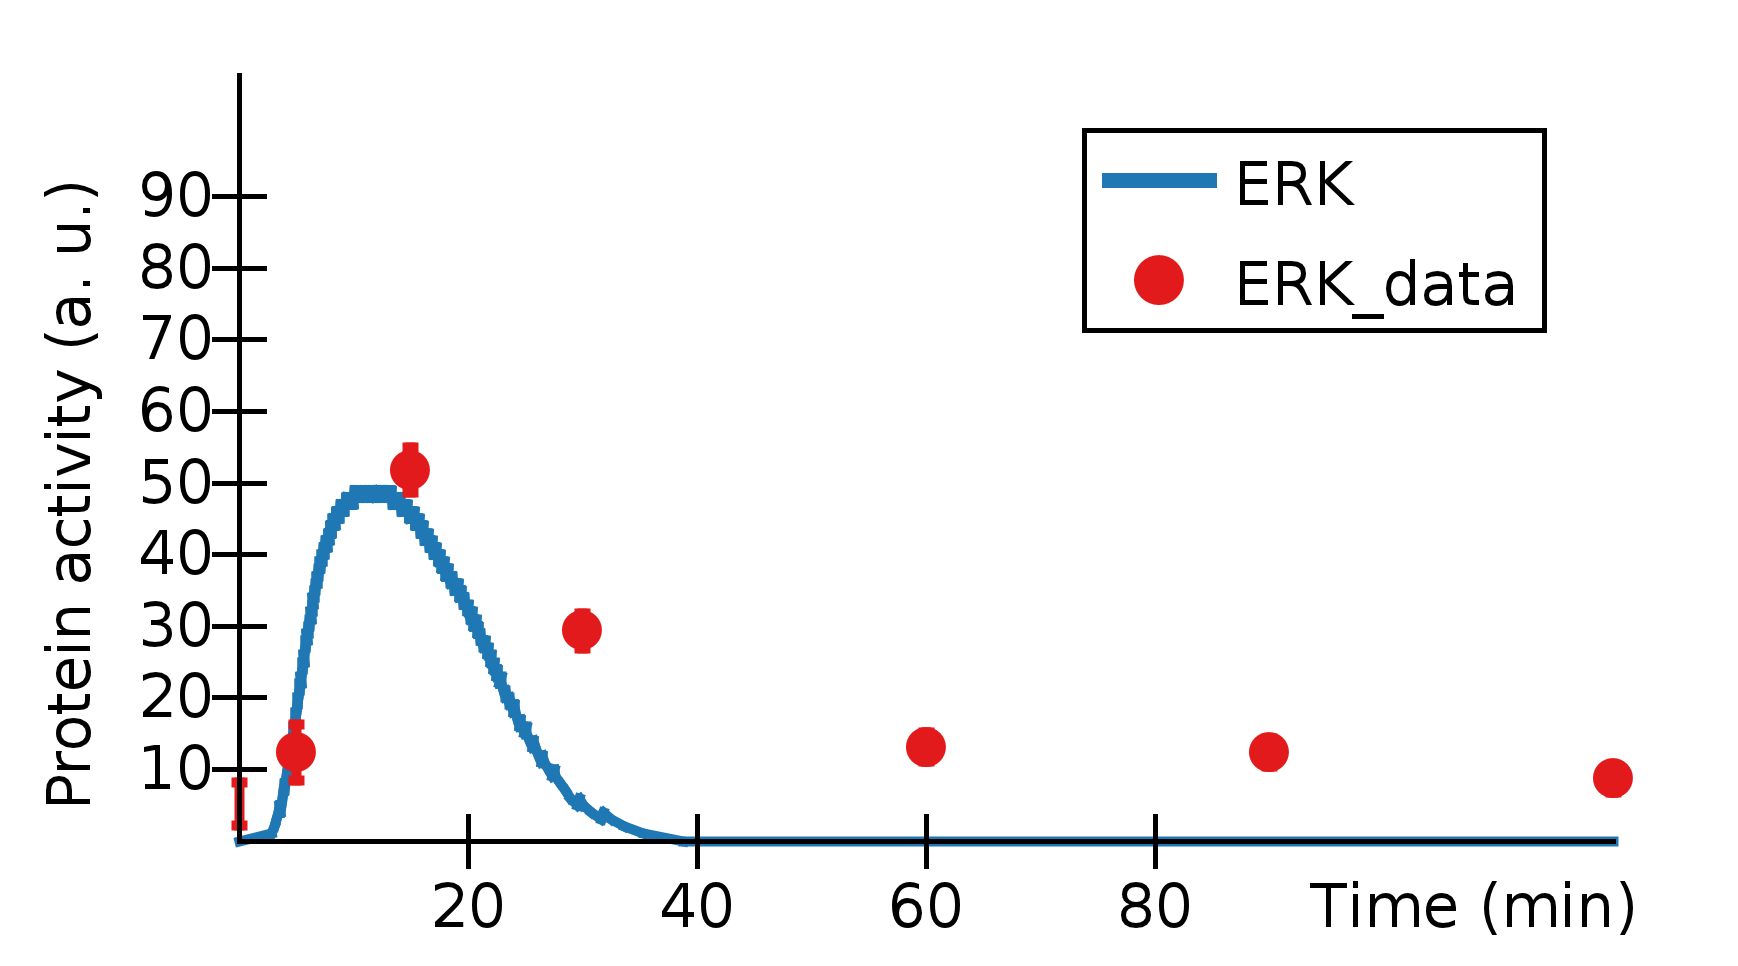
\includegraphics[width=0.29\textwidth]{images/TNFa100/ERK}} &
\subfloat[Akt (24 hours)]{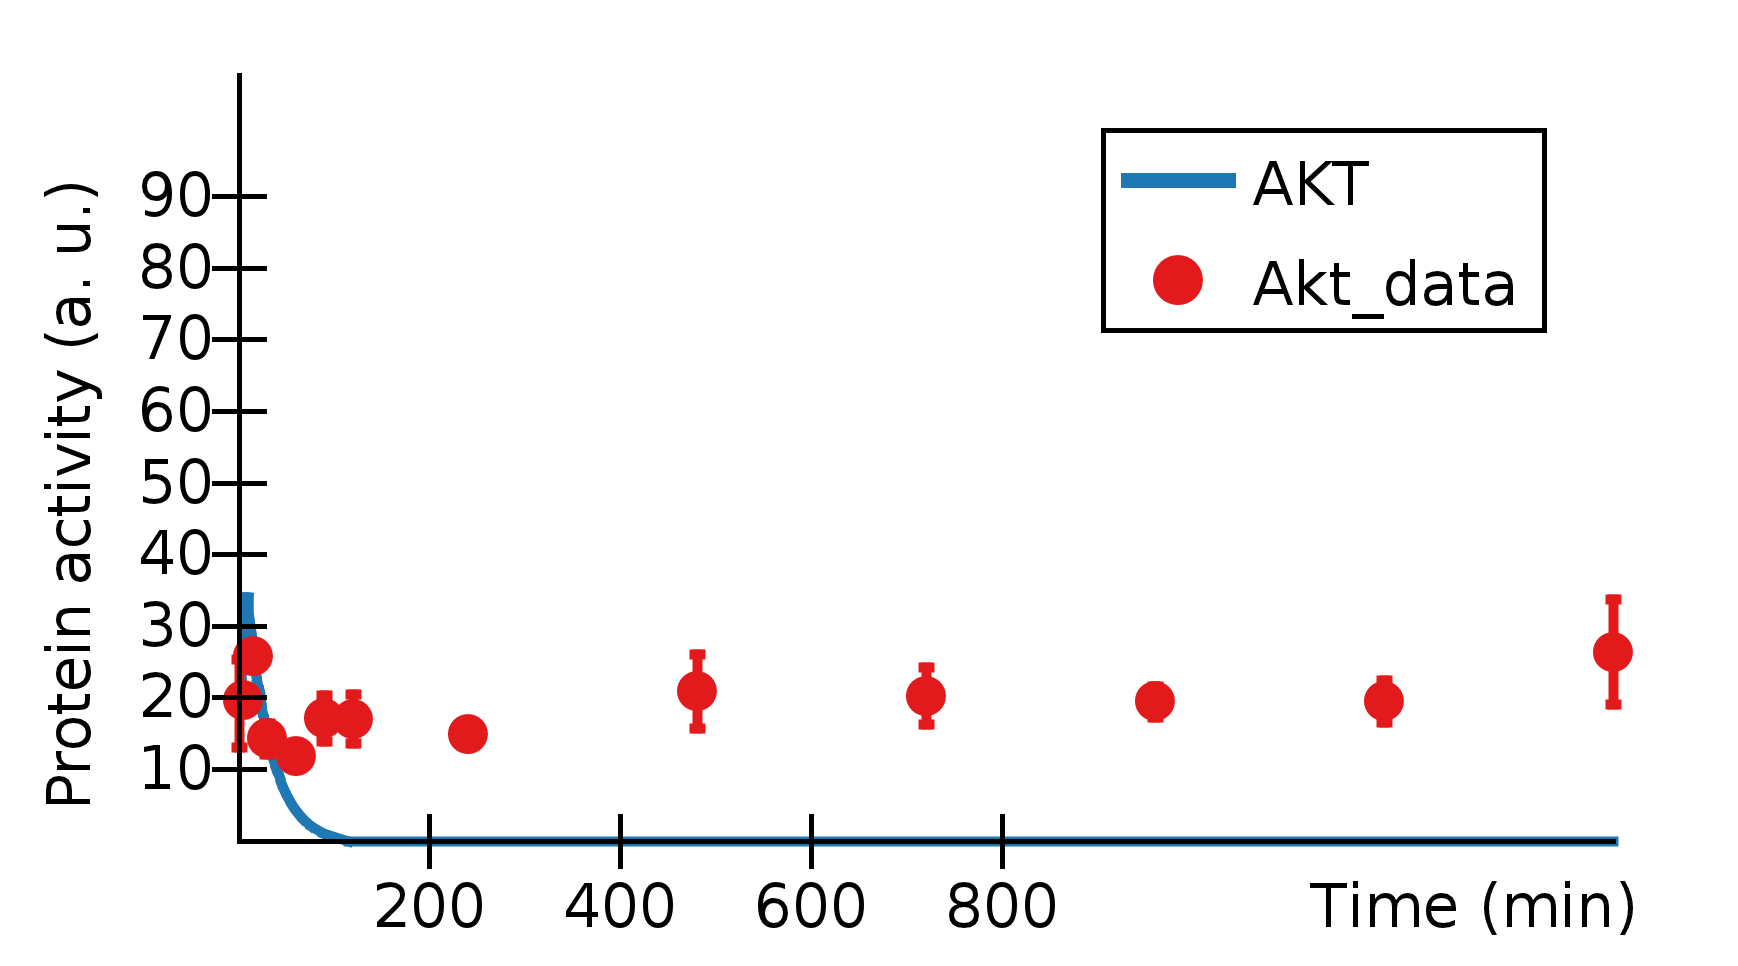
\includegraphics[width=0.29\textwidth]{images/TNFa100/Akt}} \\
\subfloat[IRS-1(S) (2 hours)]{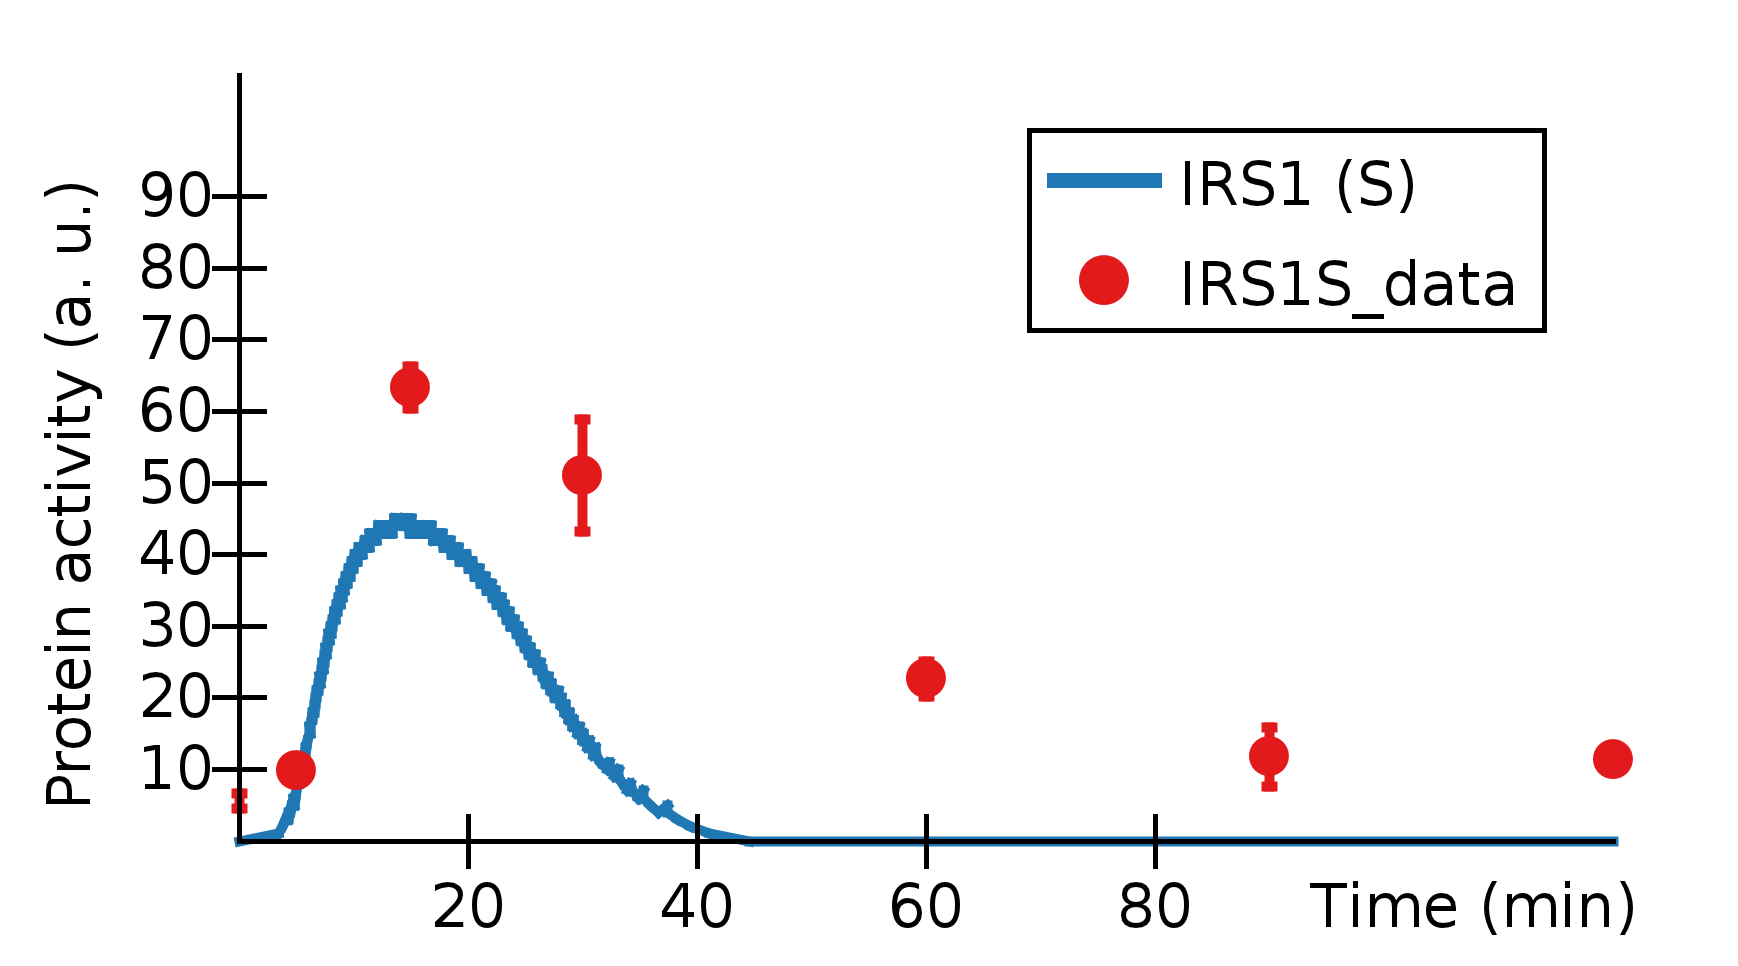
\includegraphics[width=0.29\textwidth]{images/TNFa100/IRS1s_120}} &
\subfloat[IRS-1(Y) (2 hours)]{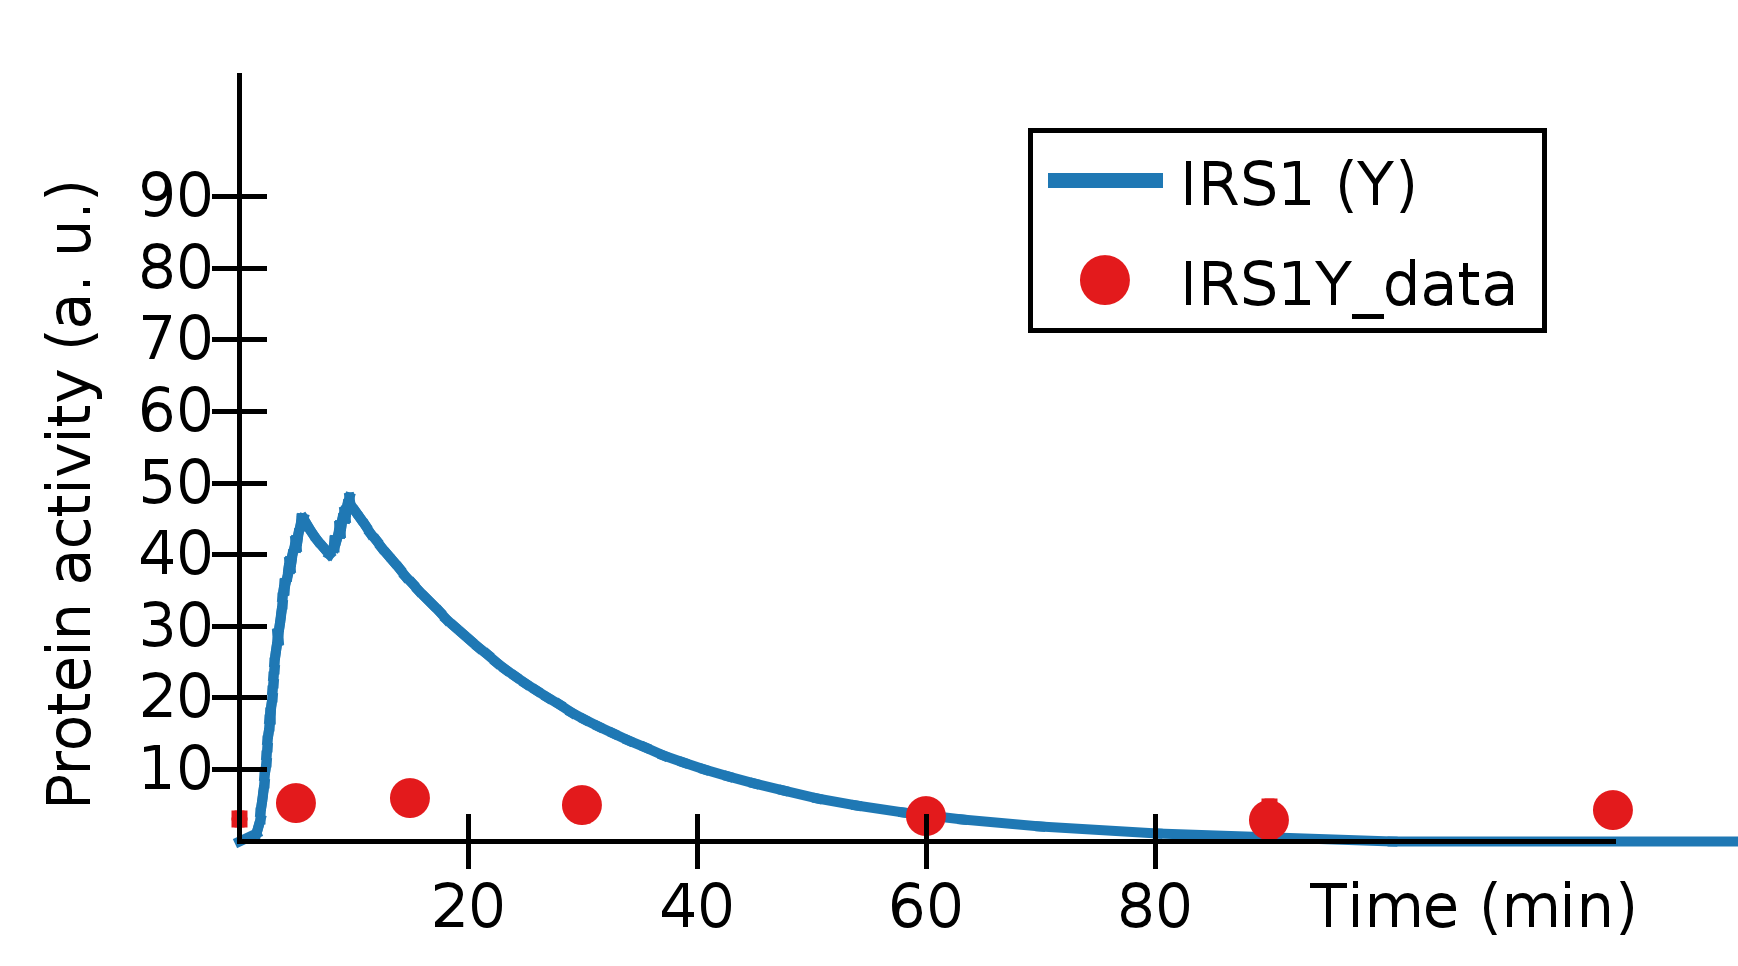
\includegraphics[width=0.29\textwidth]{images/TNFa100/IRS1y_120}} &
\subfloat[FKHR (12 hours)]{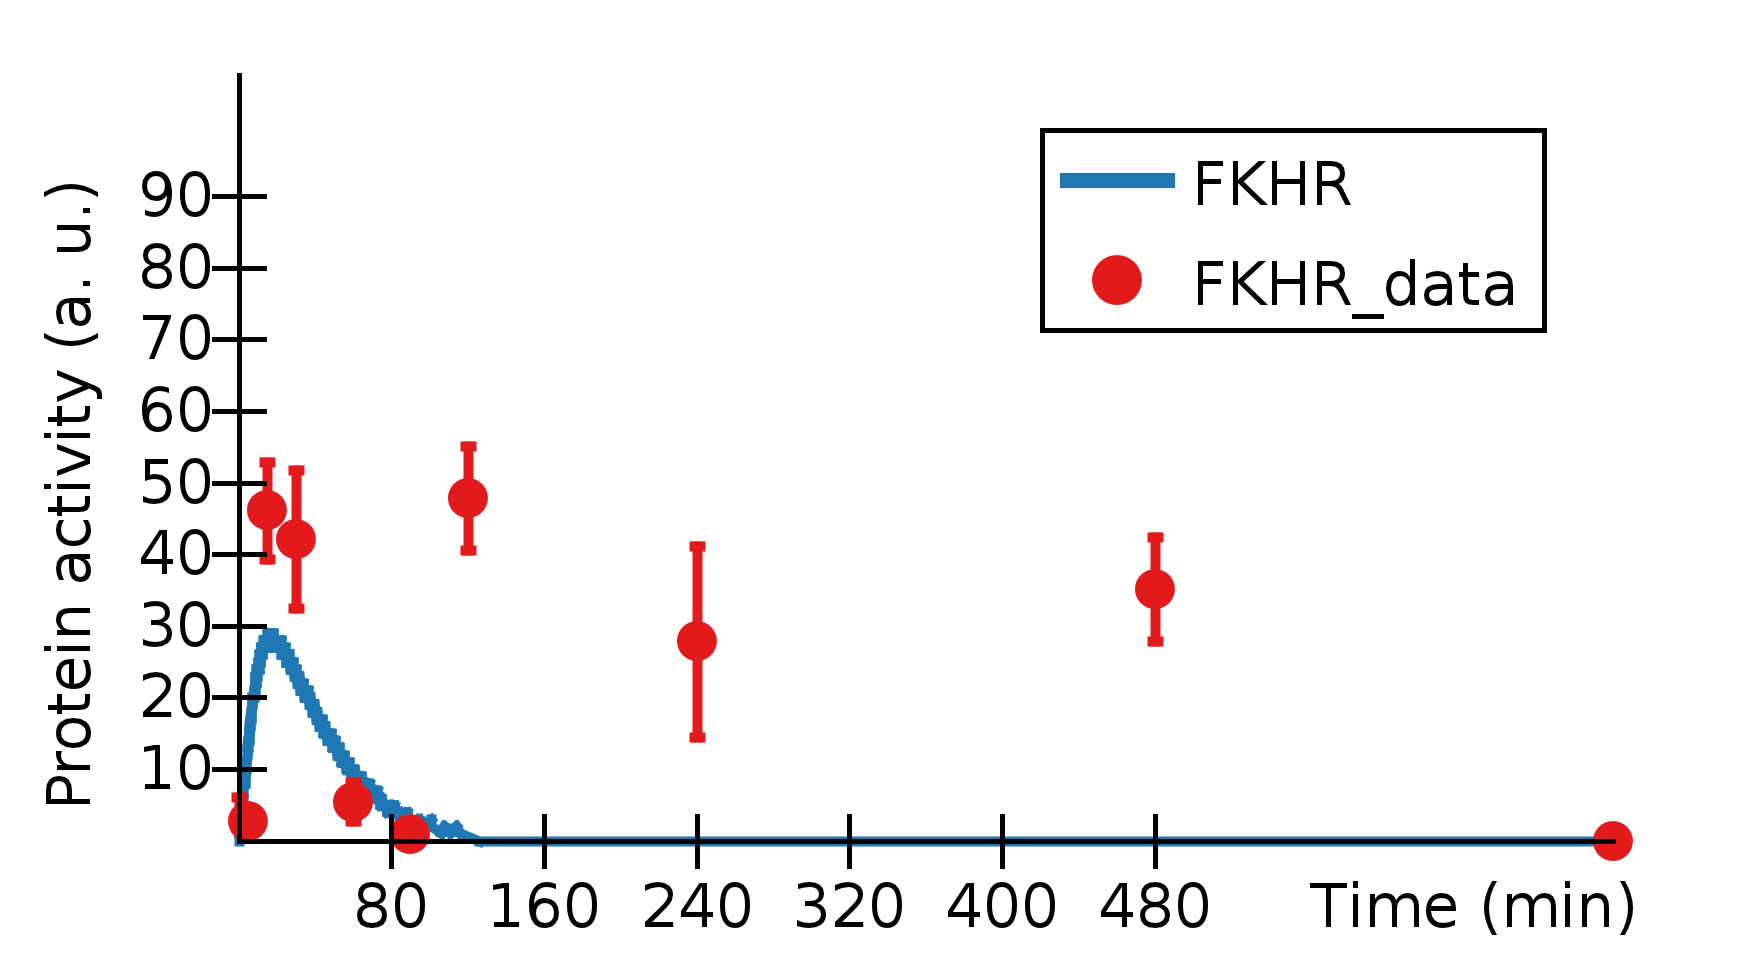
\includegraphics[width=0.29\textwidth]{images/TNFa100/FKHR_720}}
\end{tabularx}
\caption{Comparison between the ANIMO model in Figure~\ref{fig:large-model-complete} and experimental data. Treatment condition: 100 ng/ml TNF$\alpha$.
In order to ease the comparison for earlier responses, the time span for those cases is less than 24 hours.}\label{fig:differences1}
\end{minipage}
\end{figure}


\begin{figure}[!tpb]
\begin{minipage}{\textwidth}
\begin{tabularx}{\textwidth}{XXX}
\subfloat[MK2 (2 hours)]{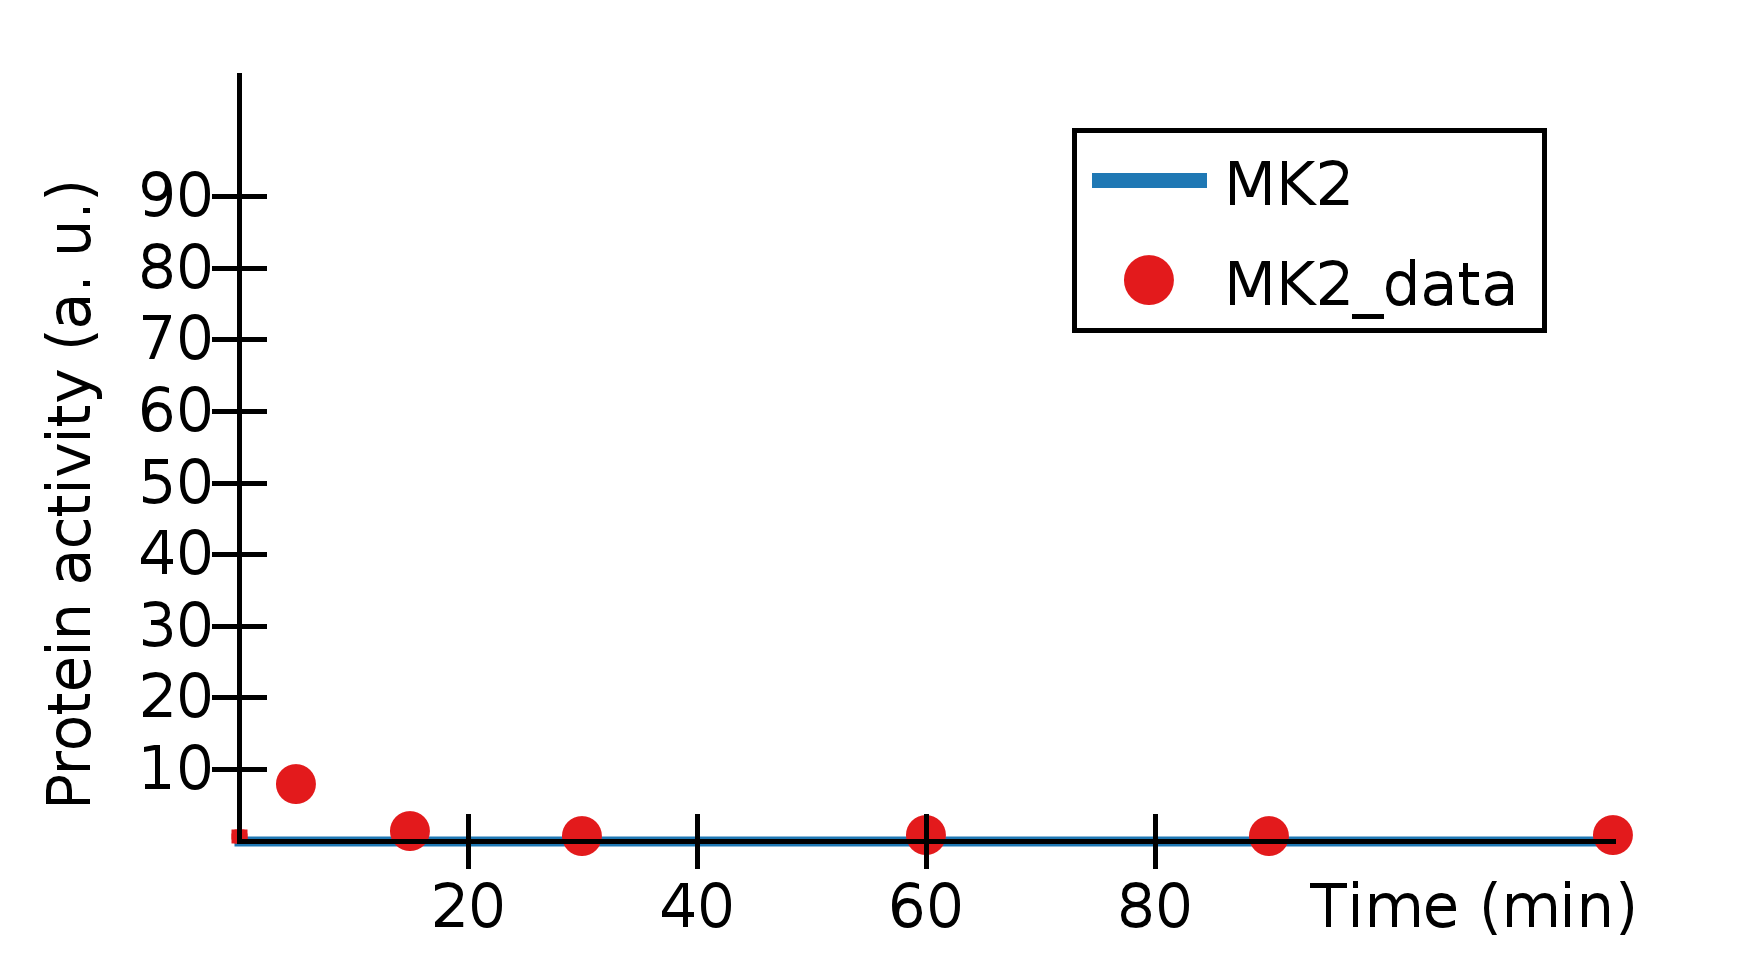
\includegraphics[width=0.29\textwidth]{images/EGF100/MK2}} &
\subfloat[JNK1 (2 hours)]{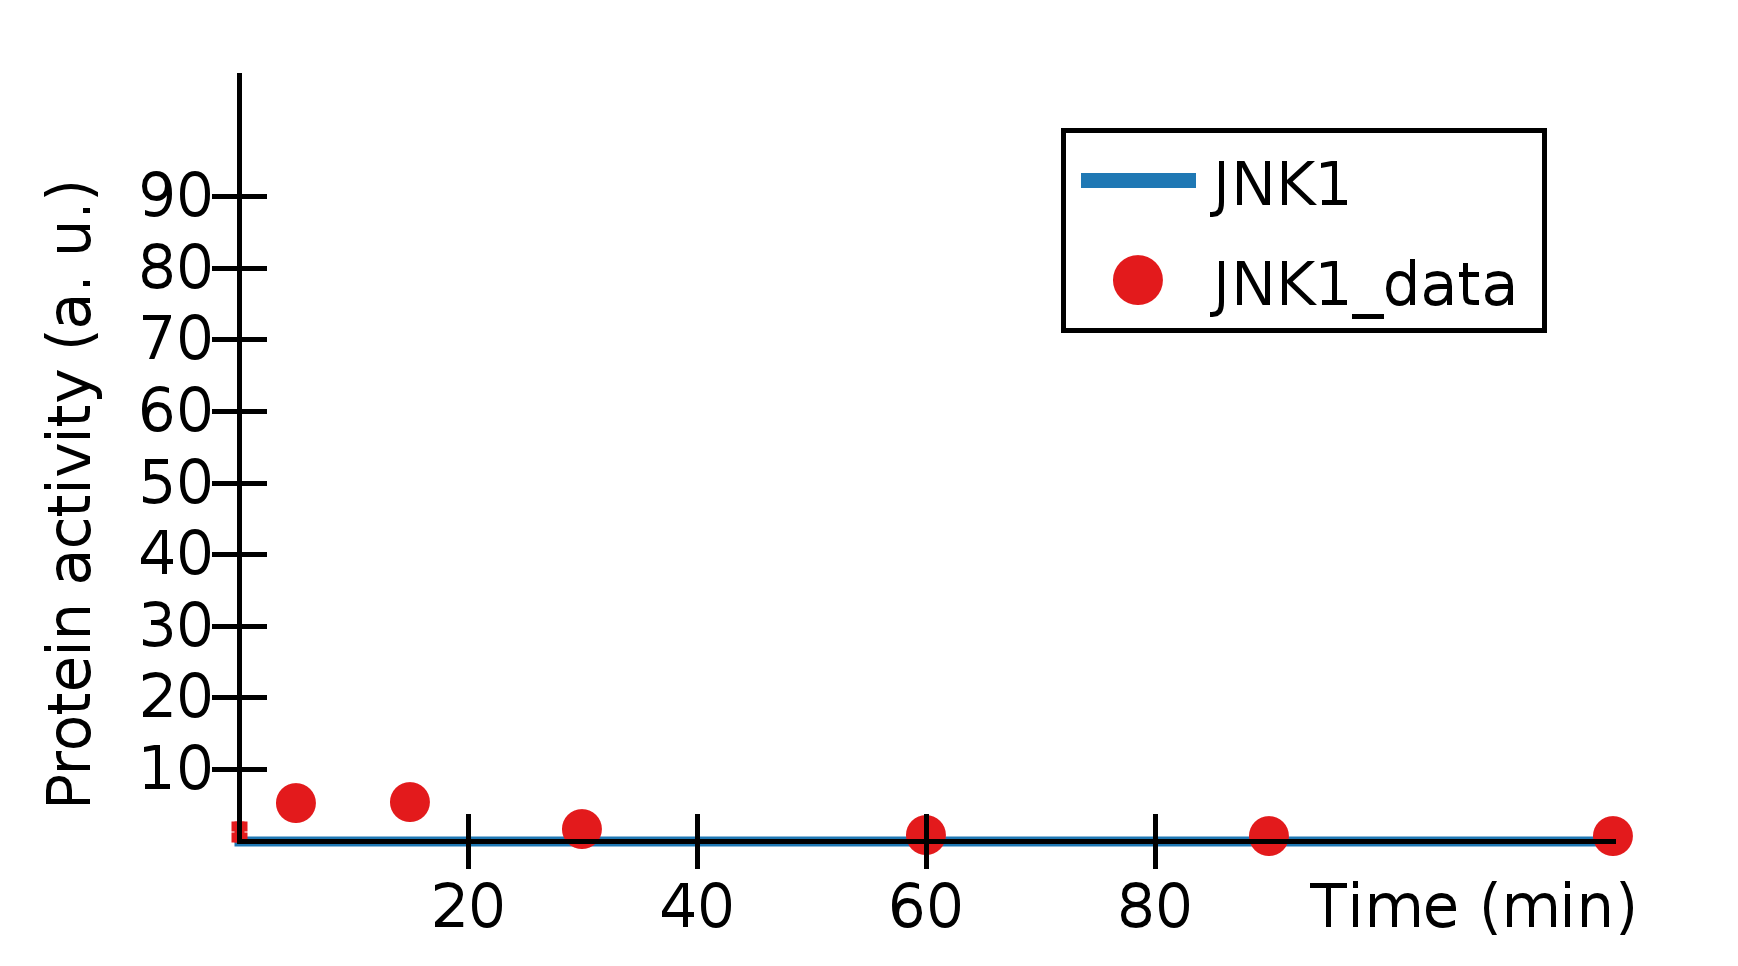
\includegraphics[width=0.29\textwidth]{images/EGF100/JNK1}} &
\subfloat[IKK (24 hours)]{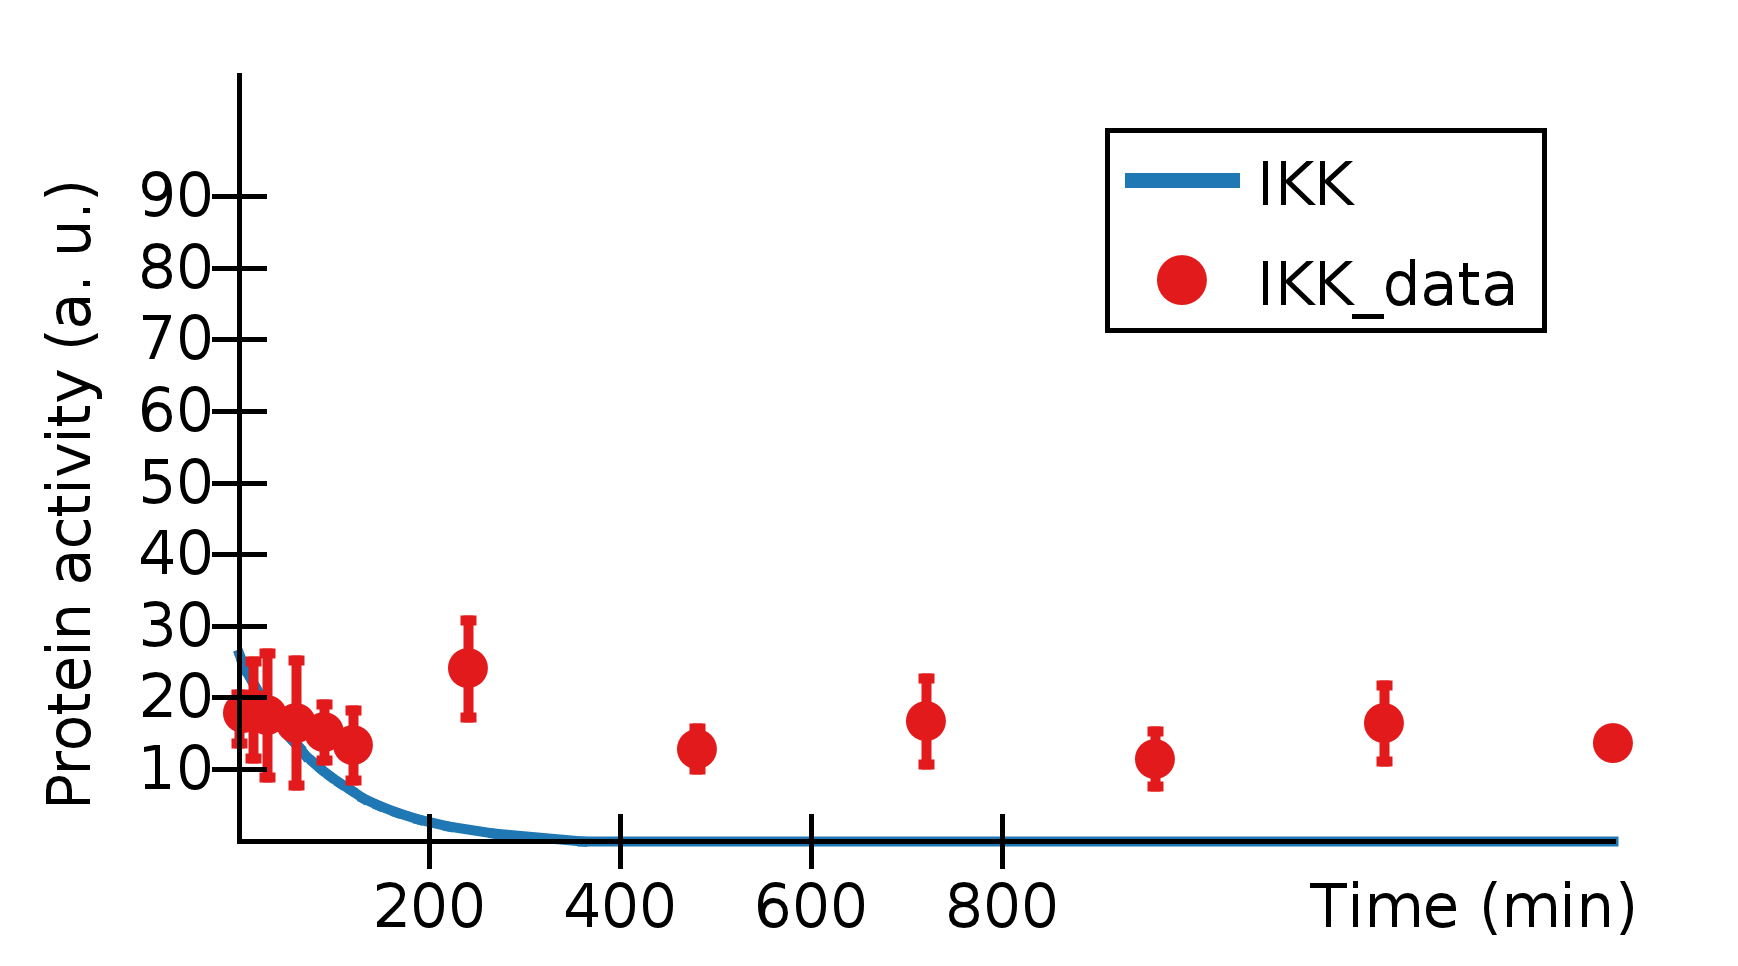
\includegraphics[width=0.29\textwidth]{images/EGF100/IKK}} \\
\subfloat[caspase-8 (24 hours)]{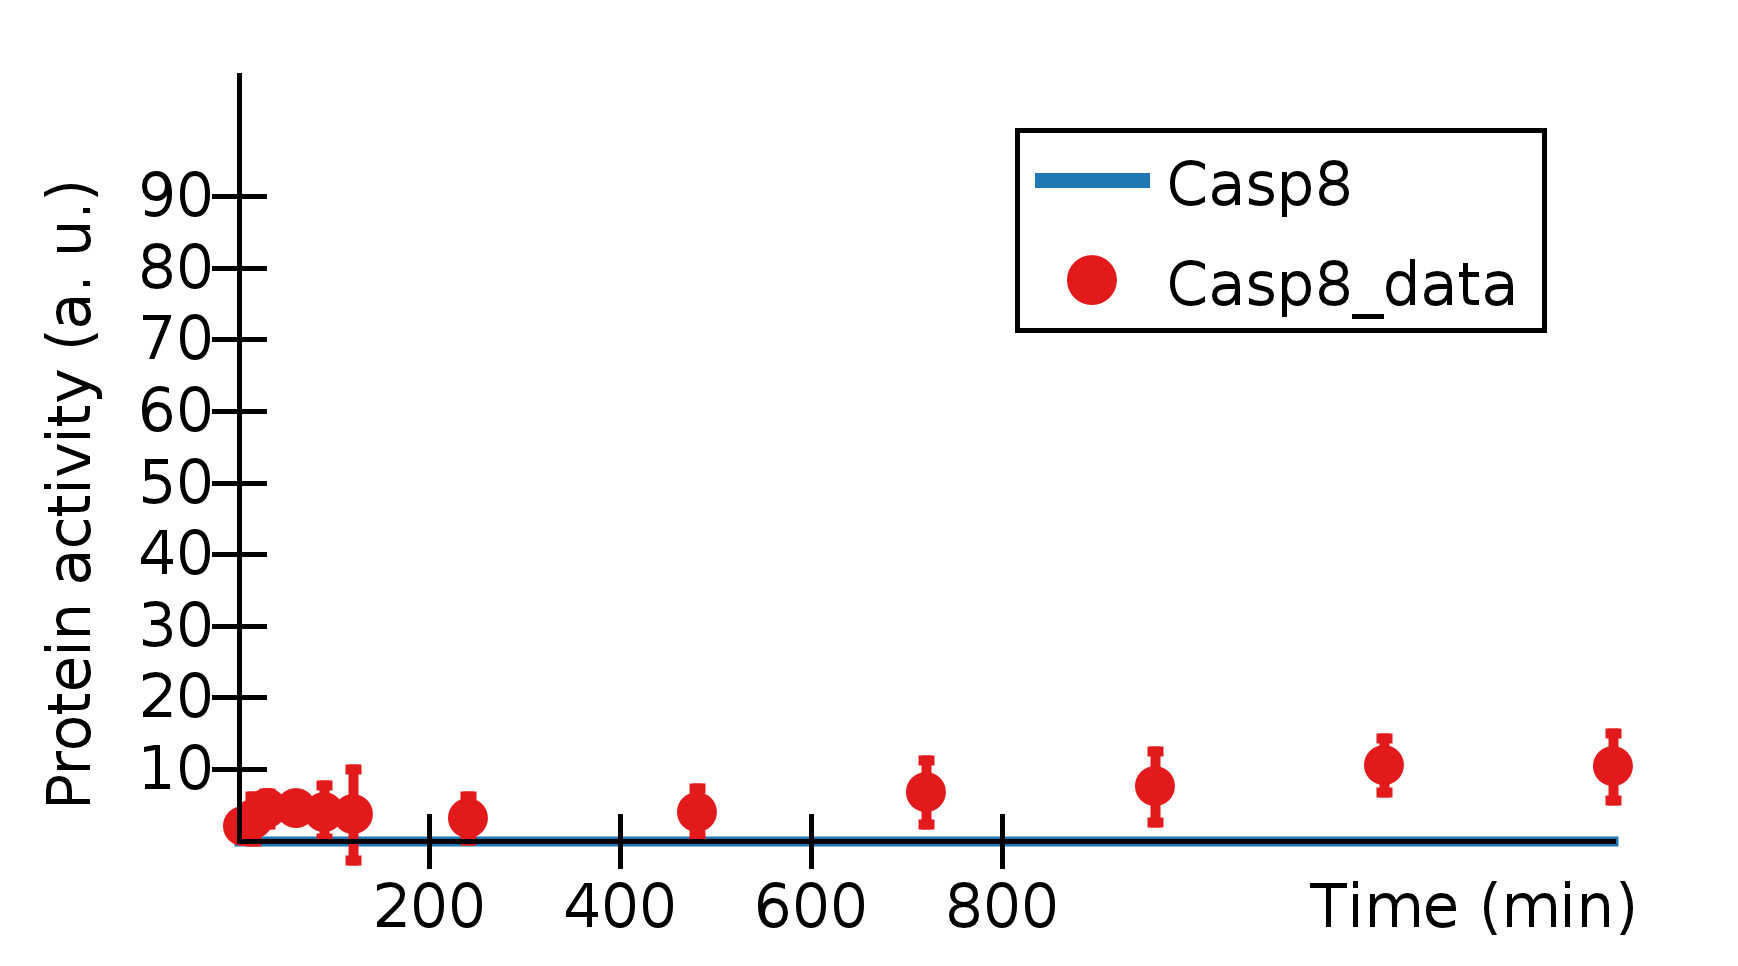
\includegraphics[width=0.29\textwidth]{images/EGF100/casp8}} &
\subfloat[caspase-3 (24 hours)]{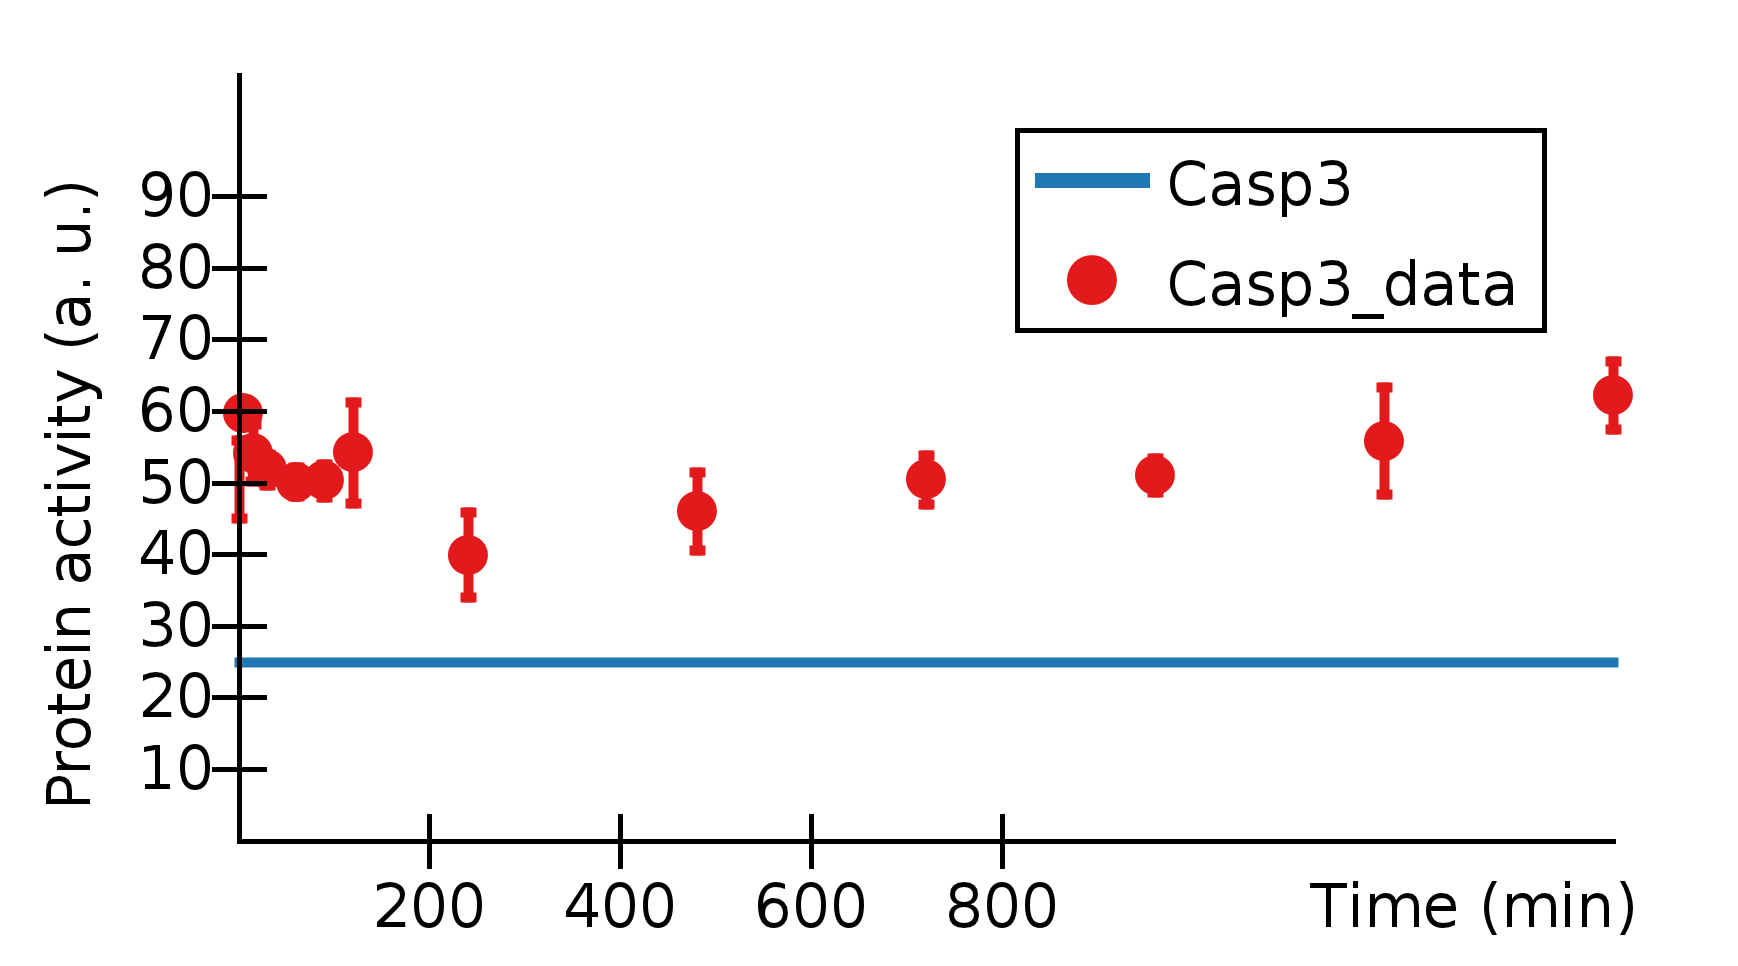
\includegraphics[width=0.29\textwidth]{images/EGF100/casp3}} &
\subfloat[MEK (2 hours)]{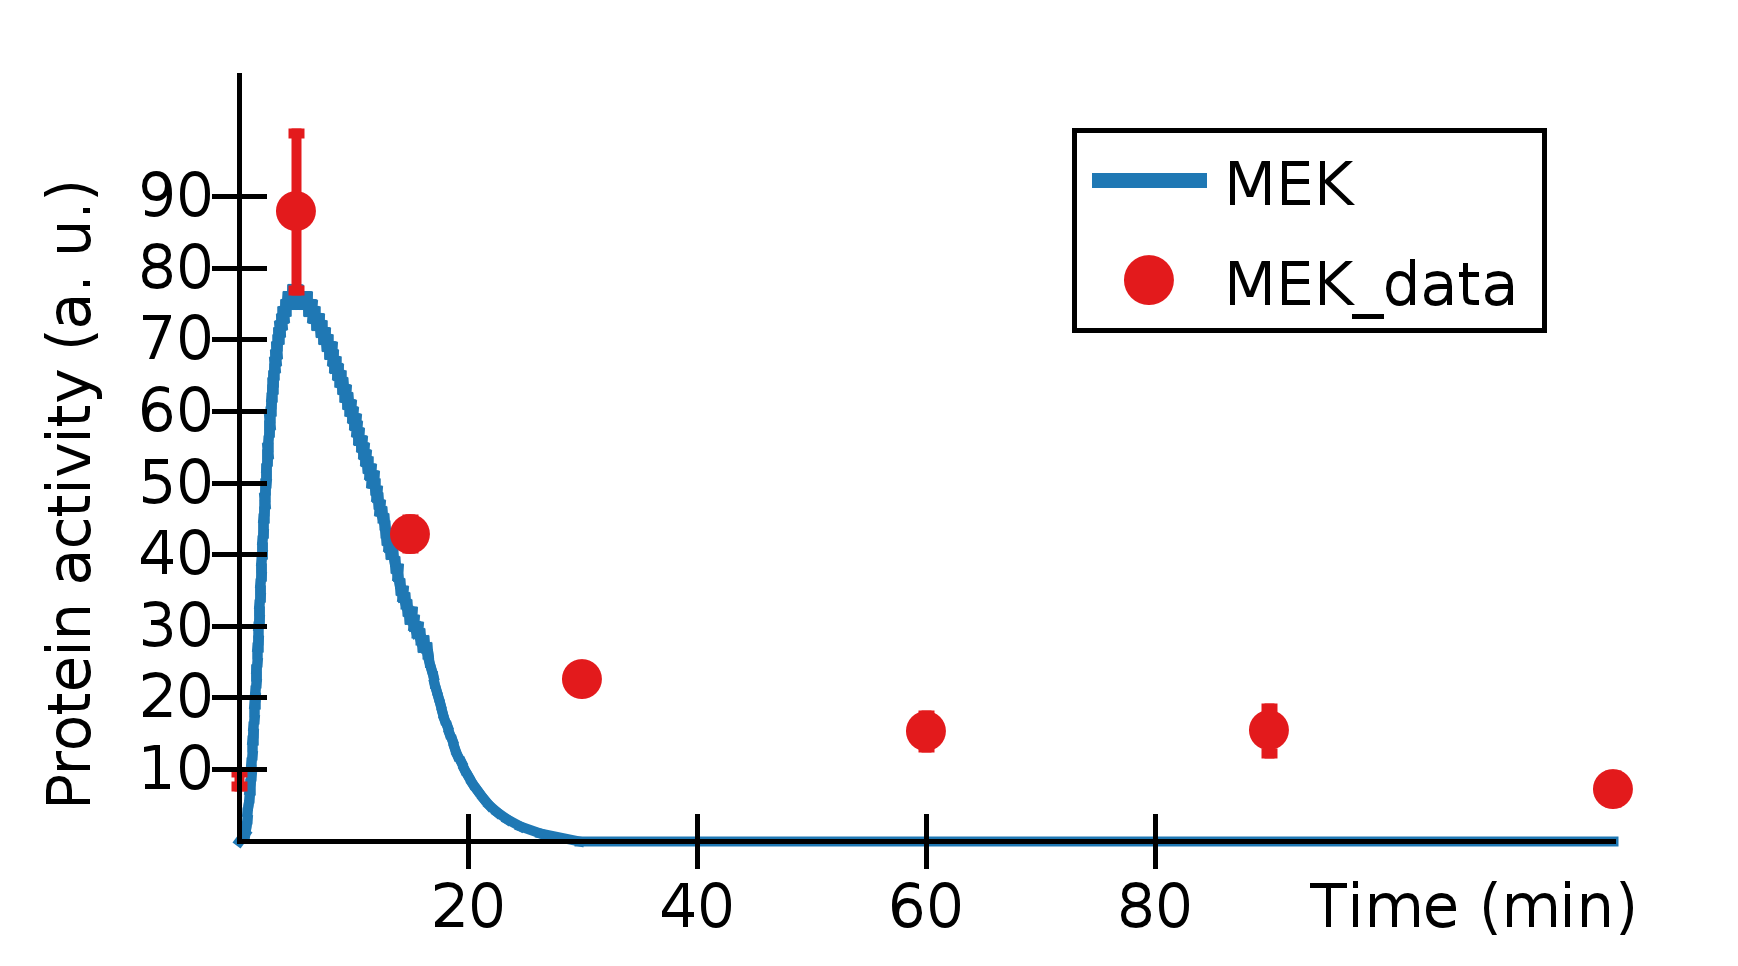
\includegraphics[width=0.29\textwidth]{images/EGF100/MEK}} \\
\subfloat[ERK (2 hours)]{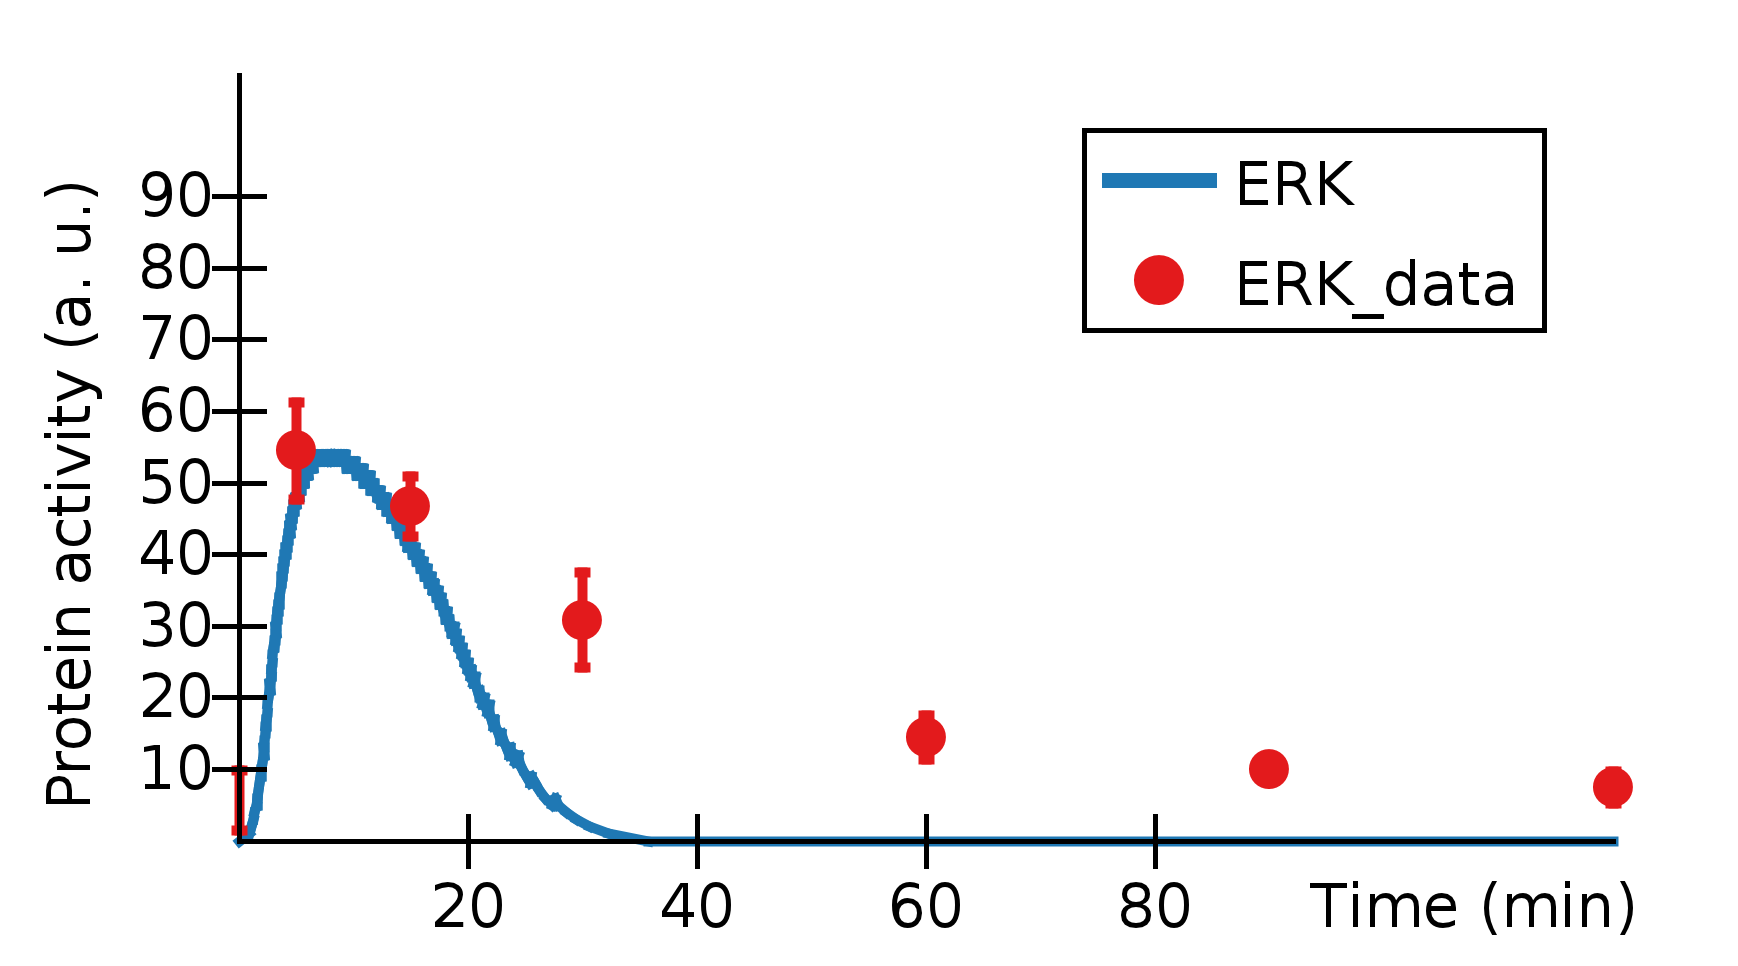
\includegraphics[width=0.29\textwidth]{images/EGF100/ERK}} &
\subfloat[Akt (2 hours)]{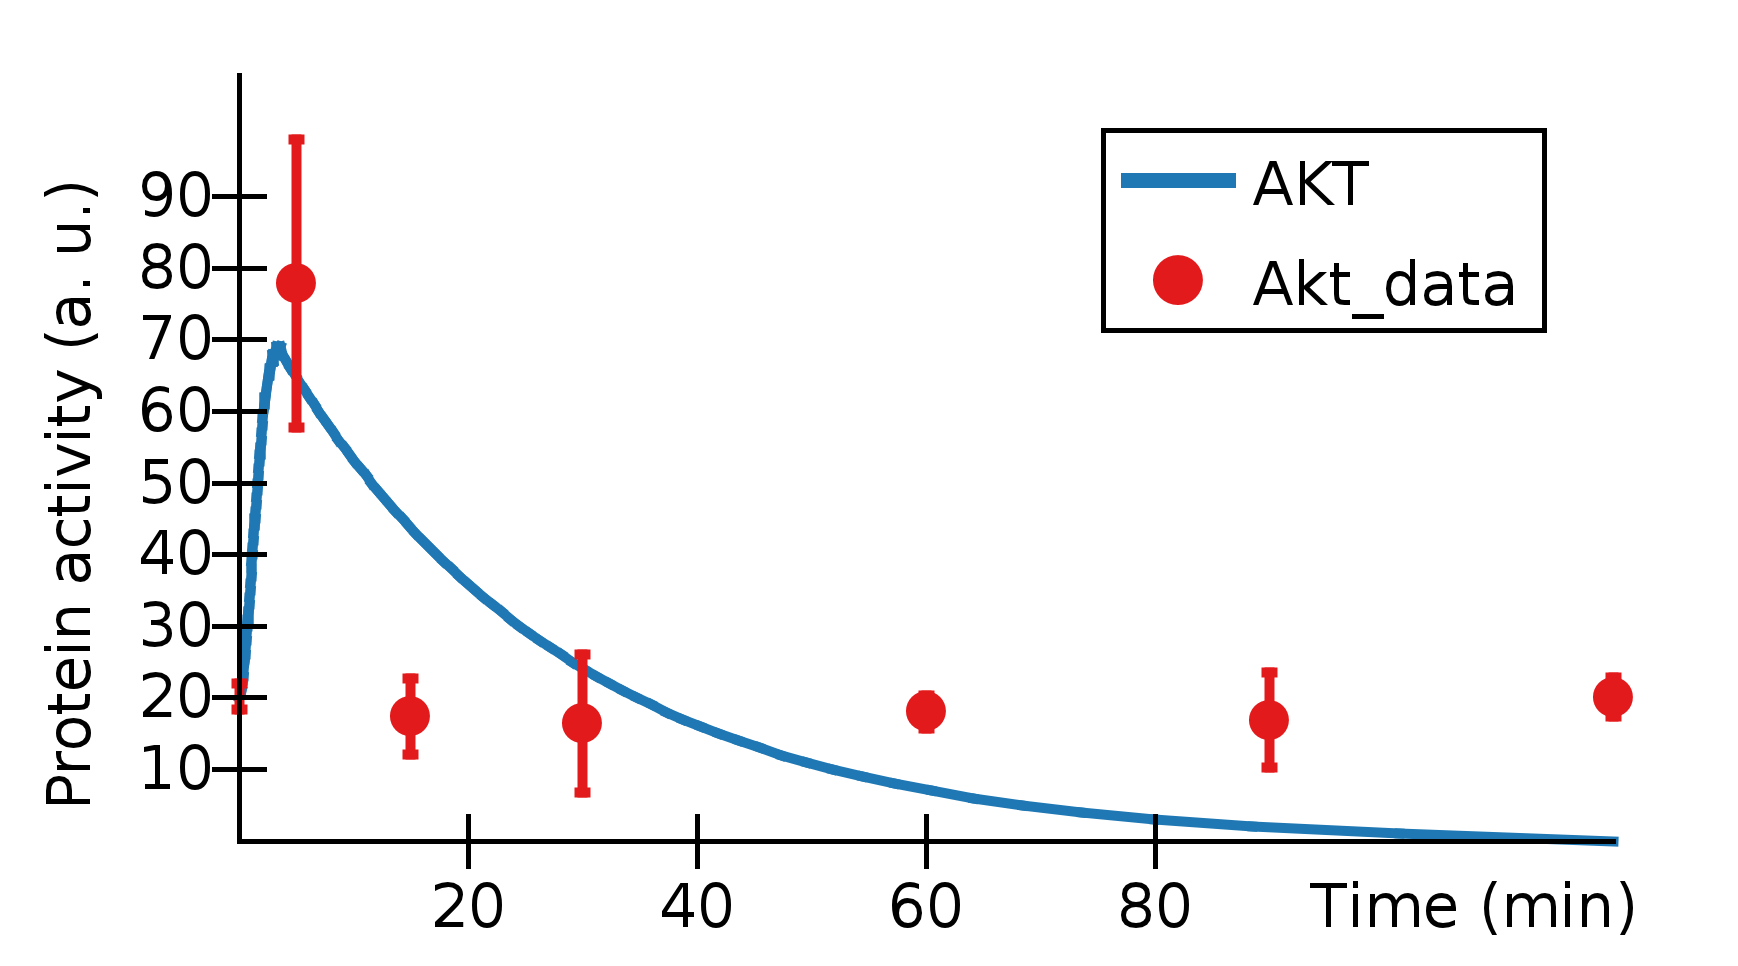
\includegraphics[width=0.29\textwidth]{images/EGF100/Akt_120}} &
\subfloat[Akt (24 hours)]{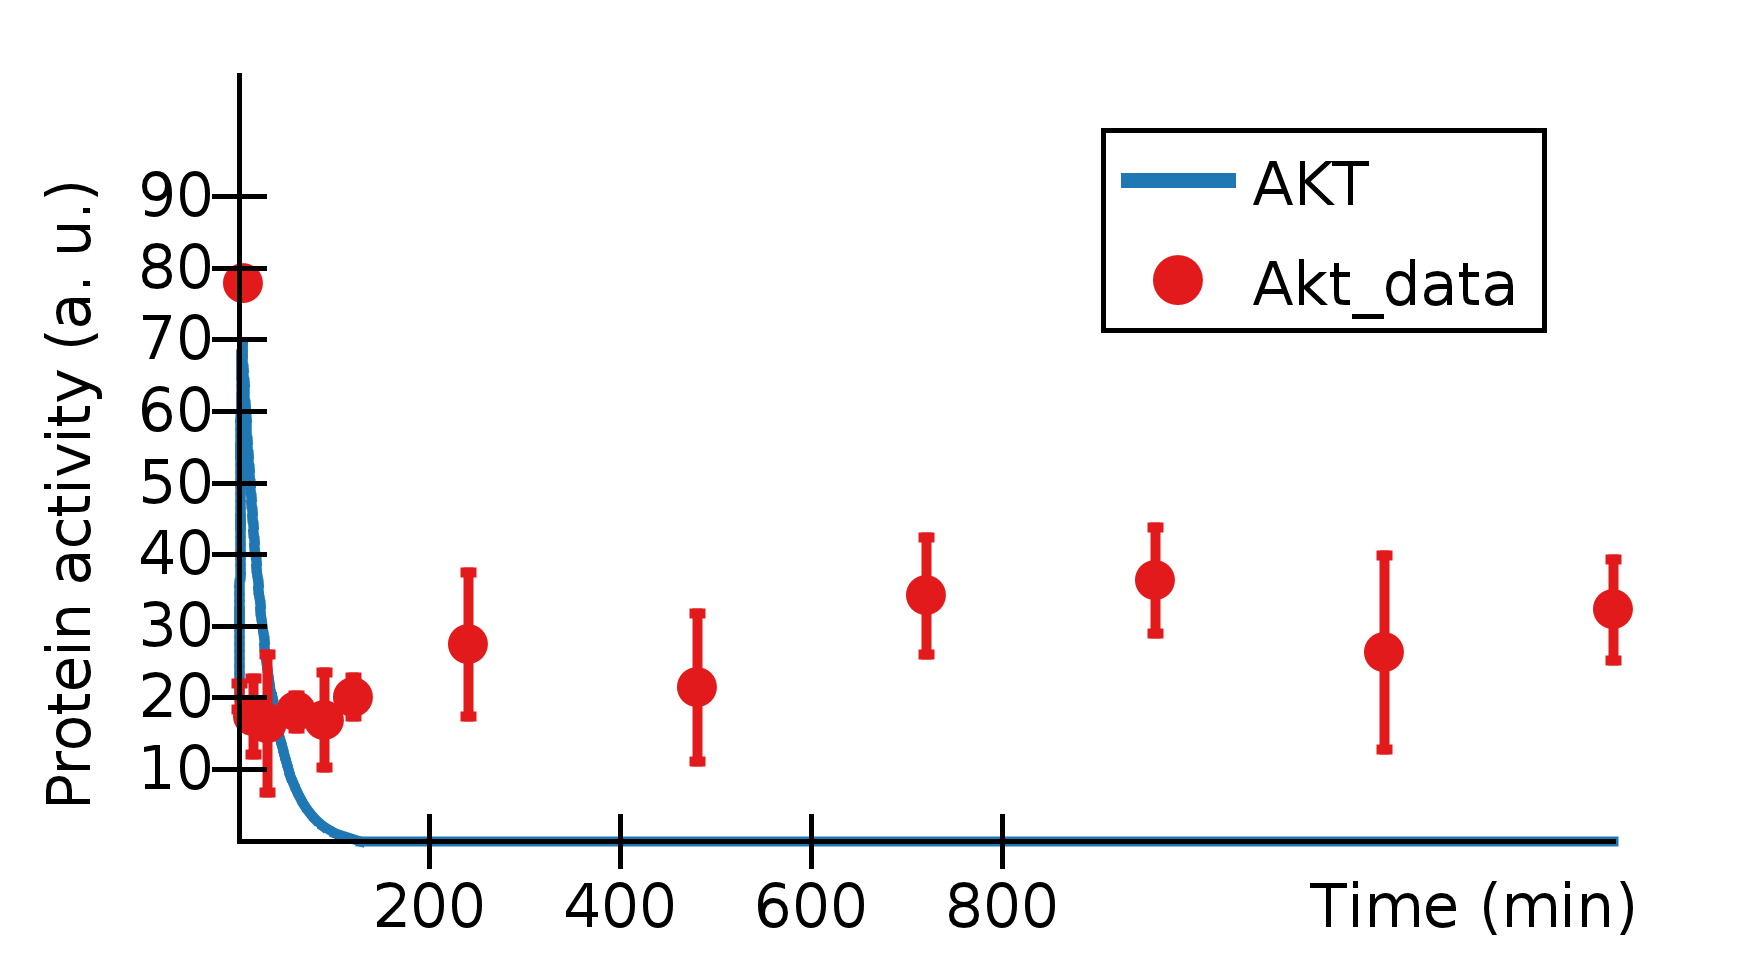
\includegraphics[width=0.29\textwidth]{images/EGF100/Akt_1440}} \\
\subfloat[IRS-1(S) (2 hours)]{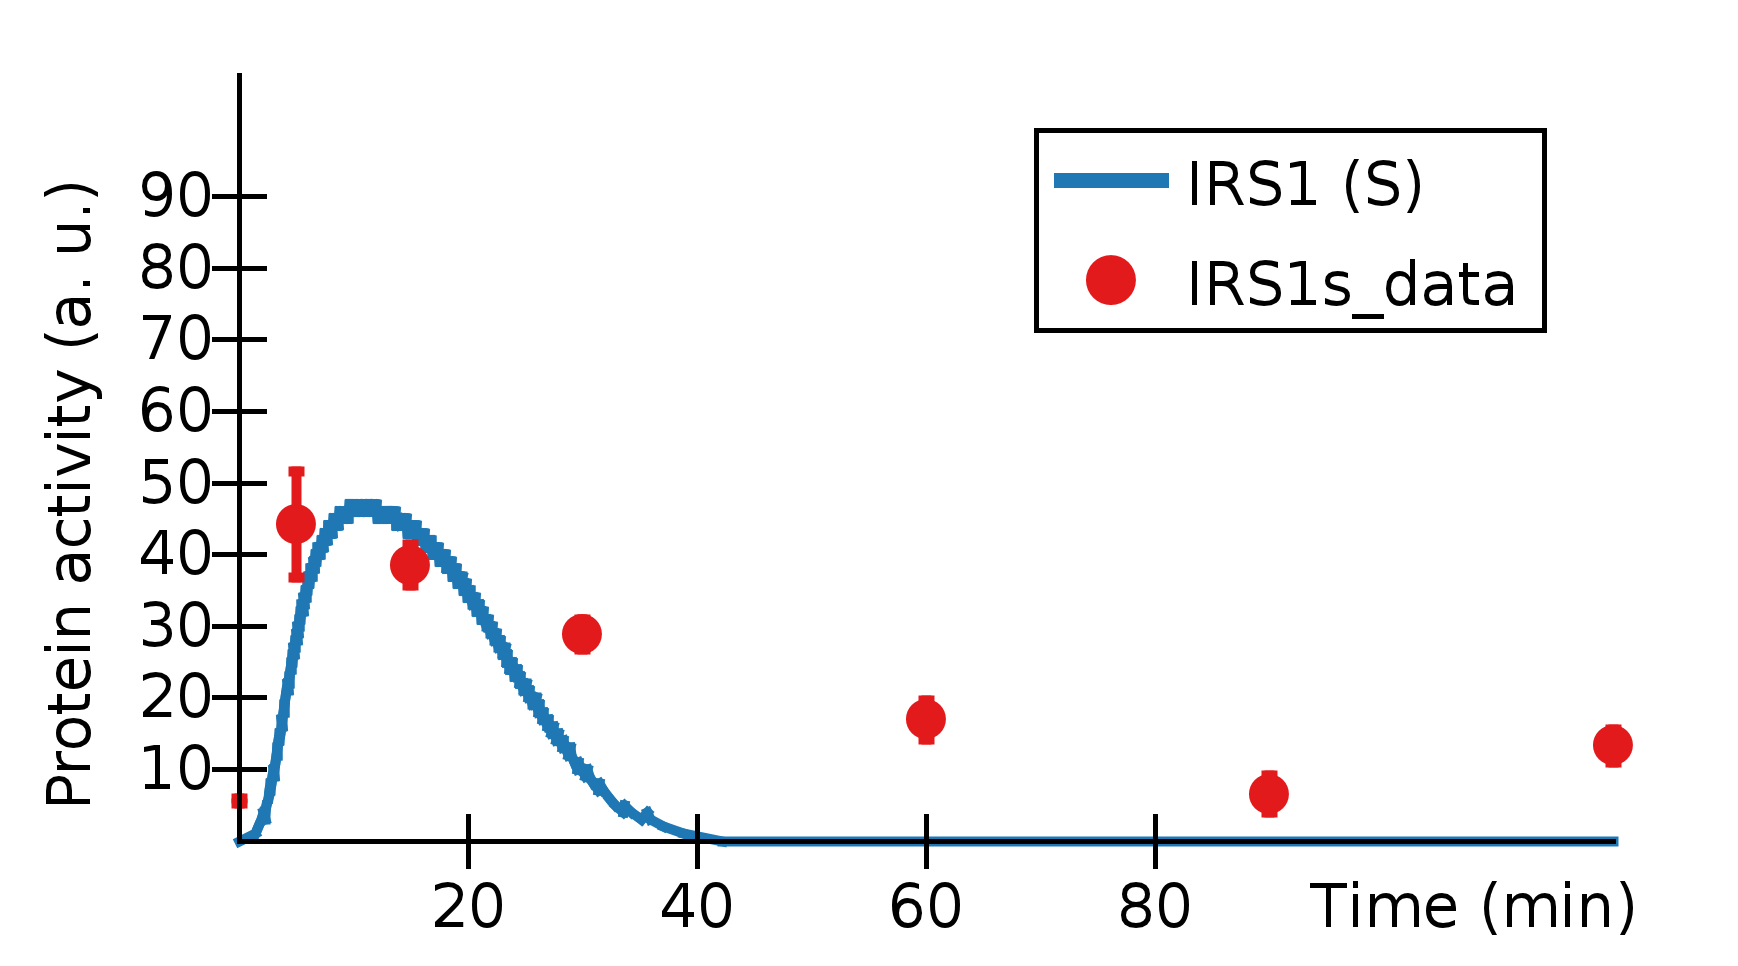
\includegraphics[width=0.29\textwidth]{images/EGF100/IRS1s_120}} &
\subfloat[IRS-1(Y) (2 hours)]{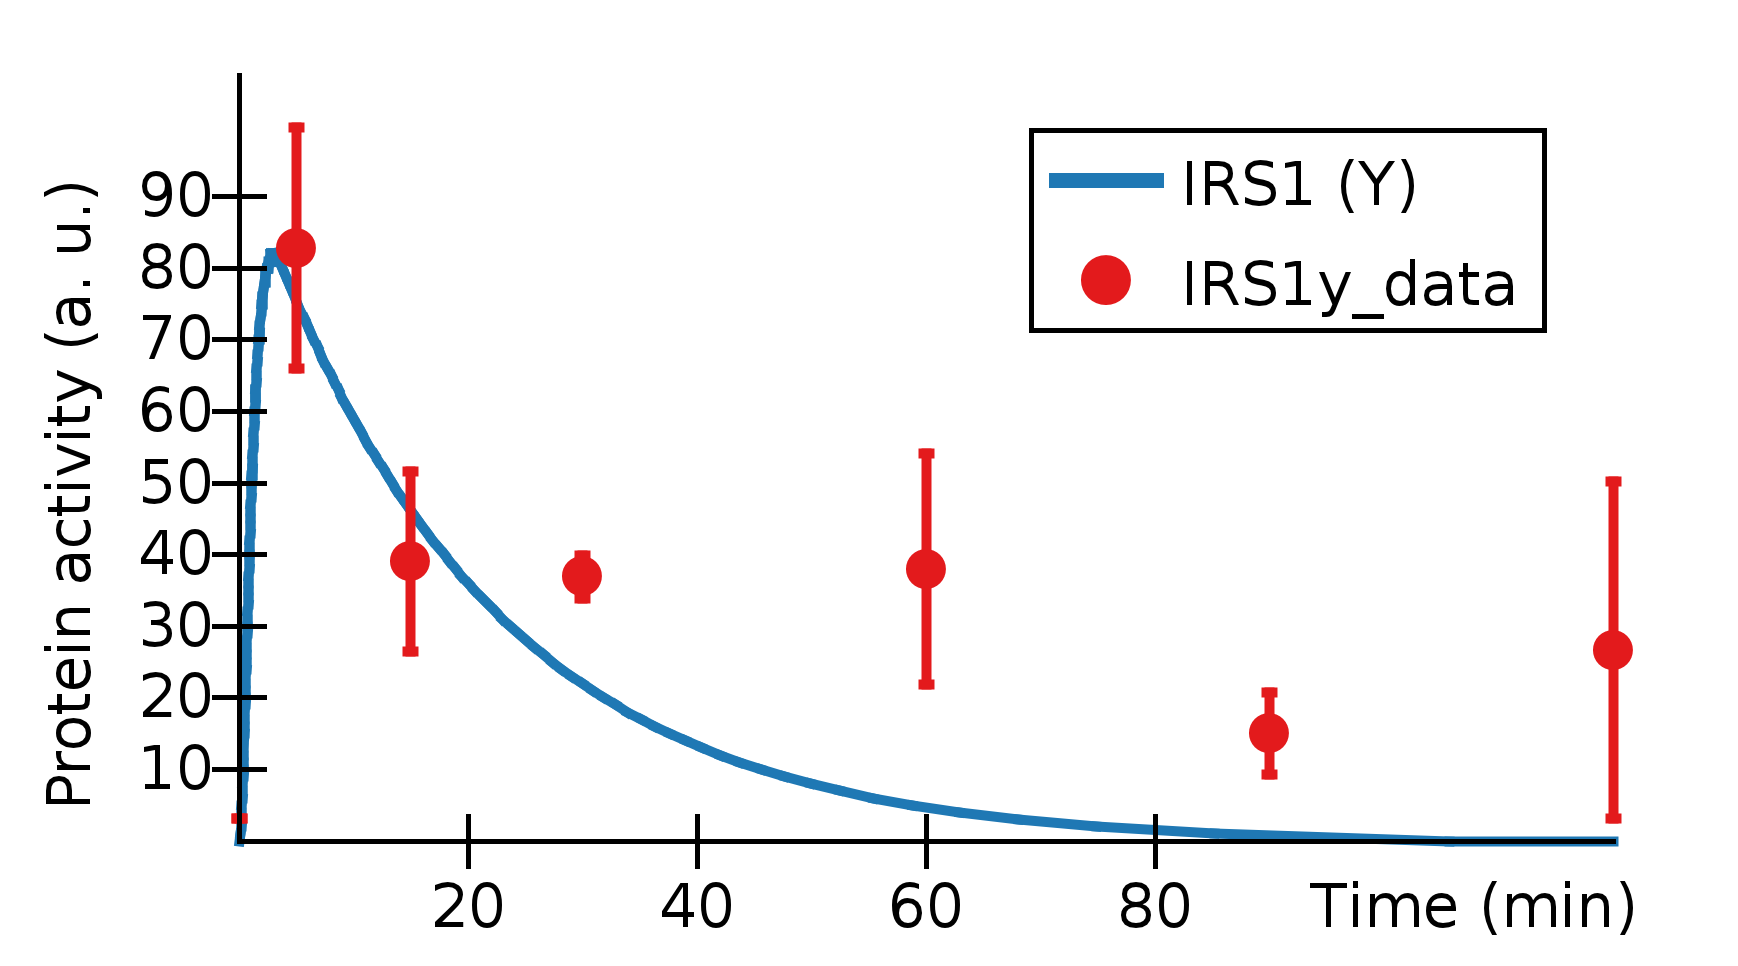
\includegraphics[width=0.29\textwidth]{images/EGF100/IRS1y_120}} &
\subfloat[IRS-1(Y) (12 hours)]{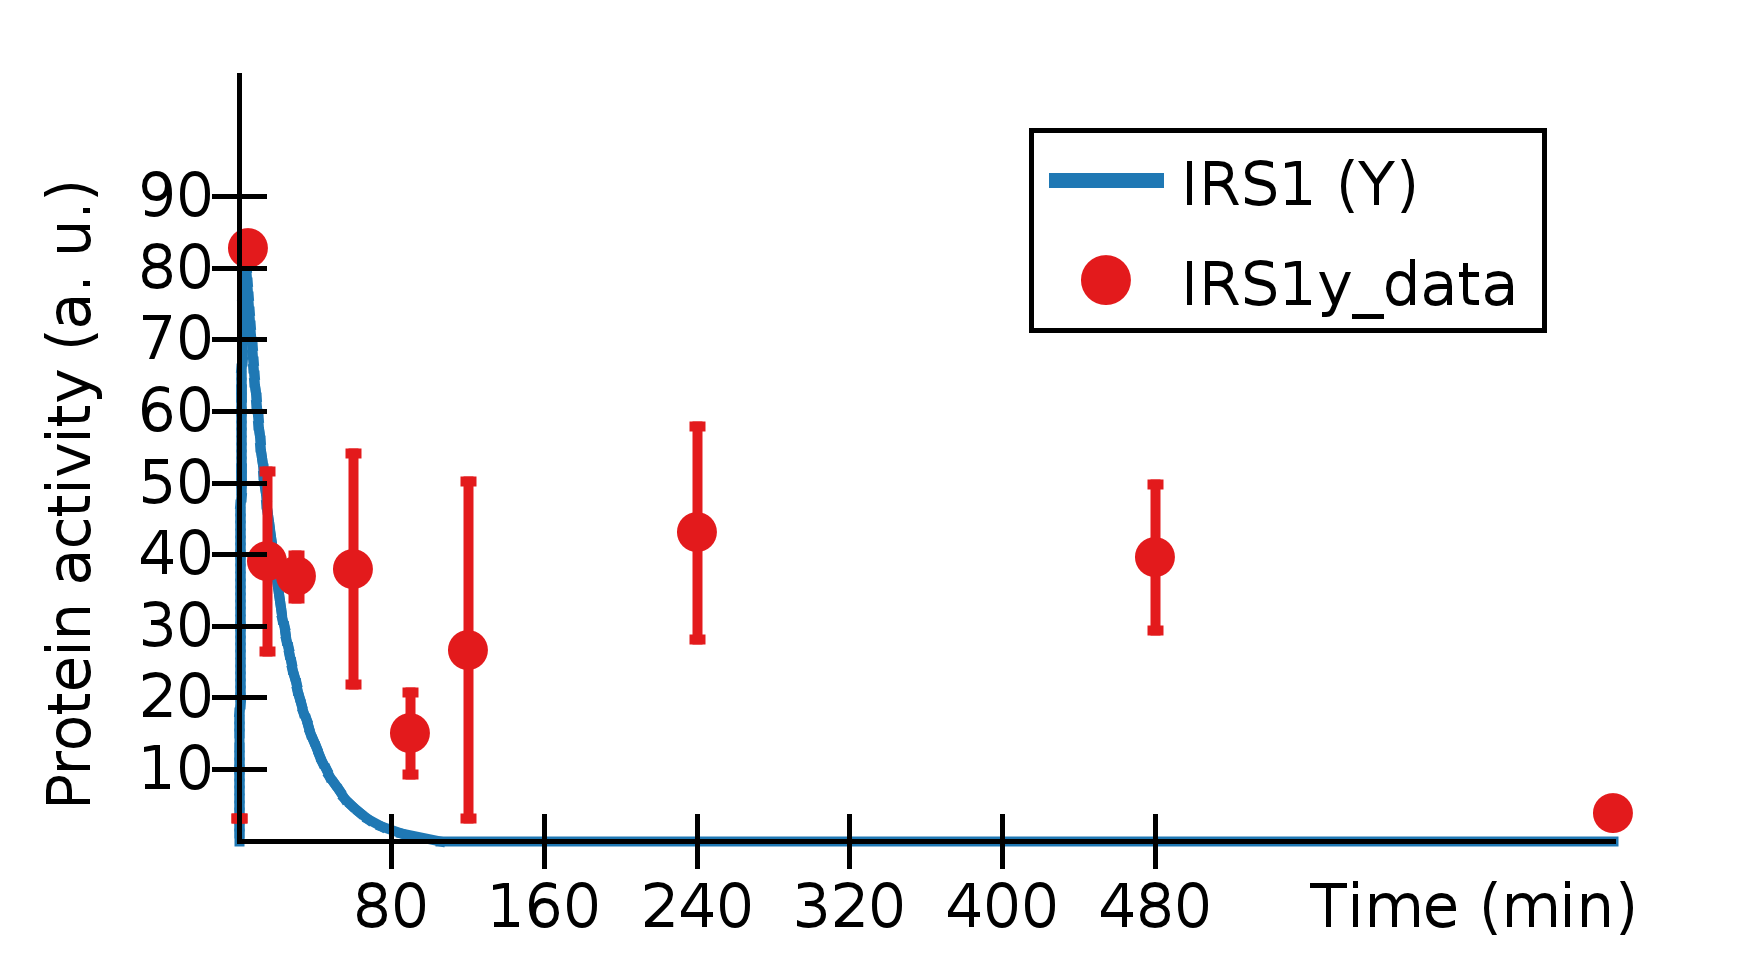
\includegraphics[width=0.29\textwidth]{images/EGF100/IRS1y_720}} \\
\subfloat[FKHR (2 hours)]{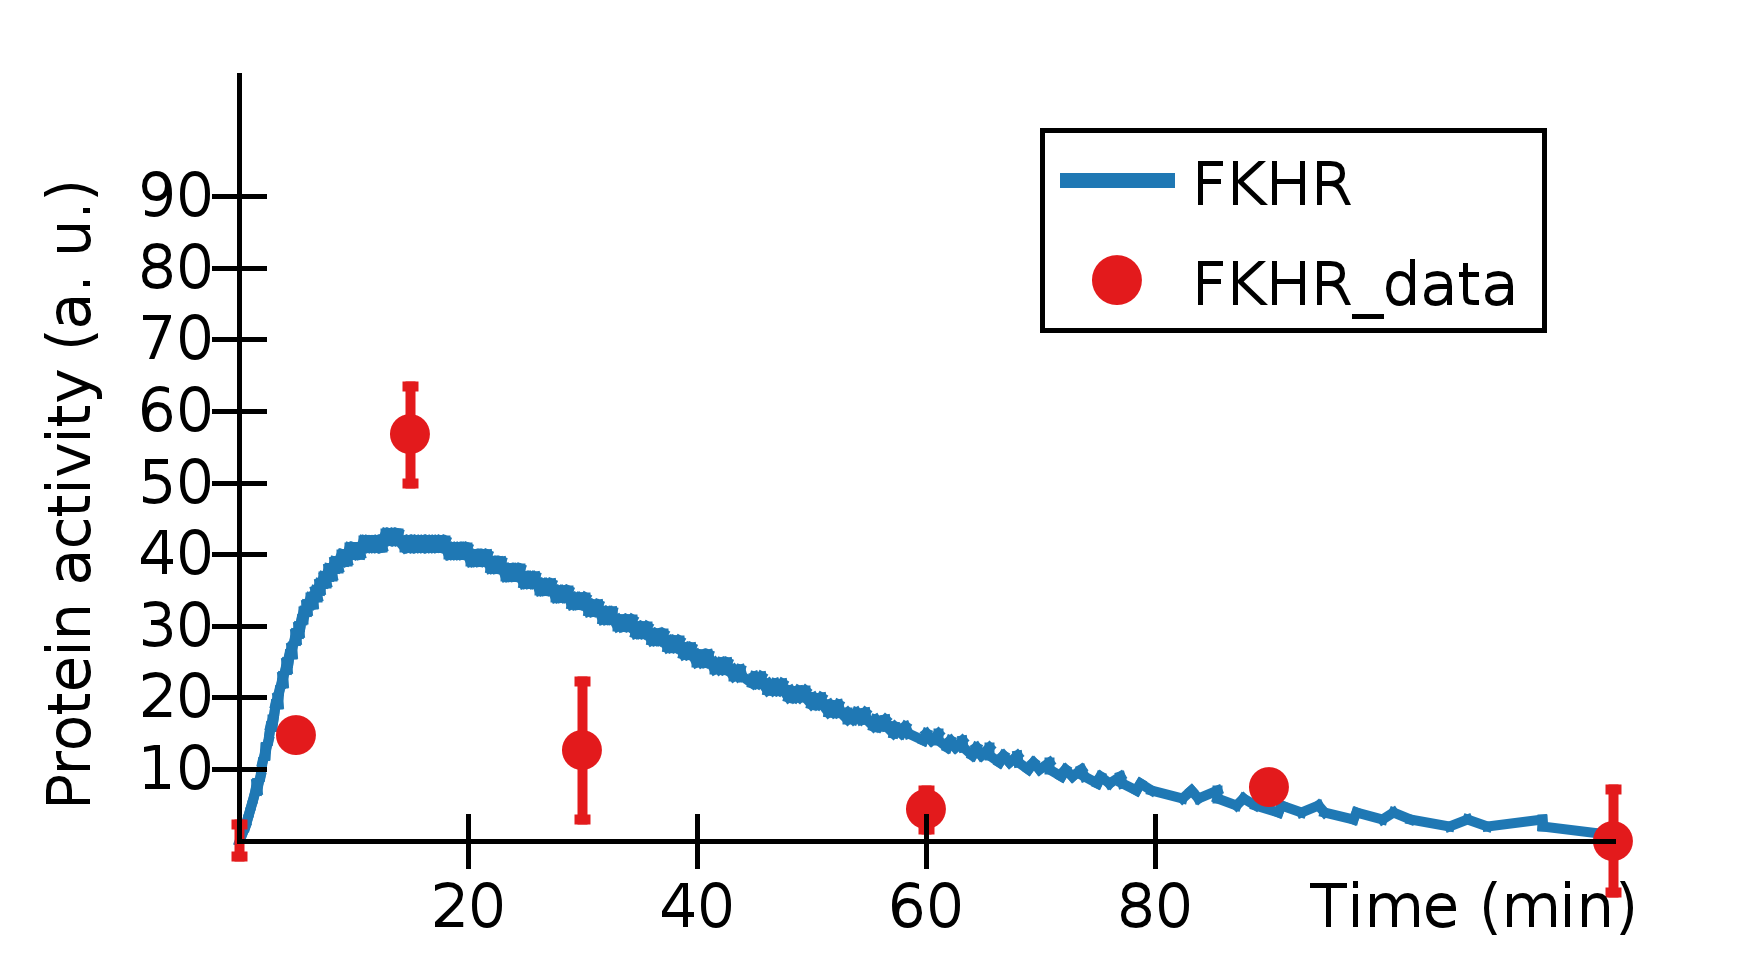
\includegraphics[width=0.29\textwidth]{images/EGF100/FKHR_120}} &
\subfloat[FKHR (12 hours)]{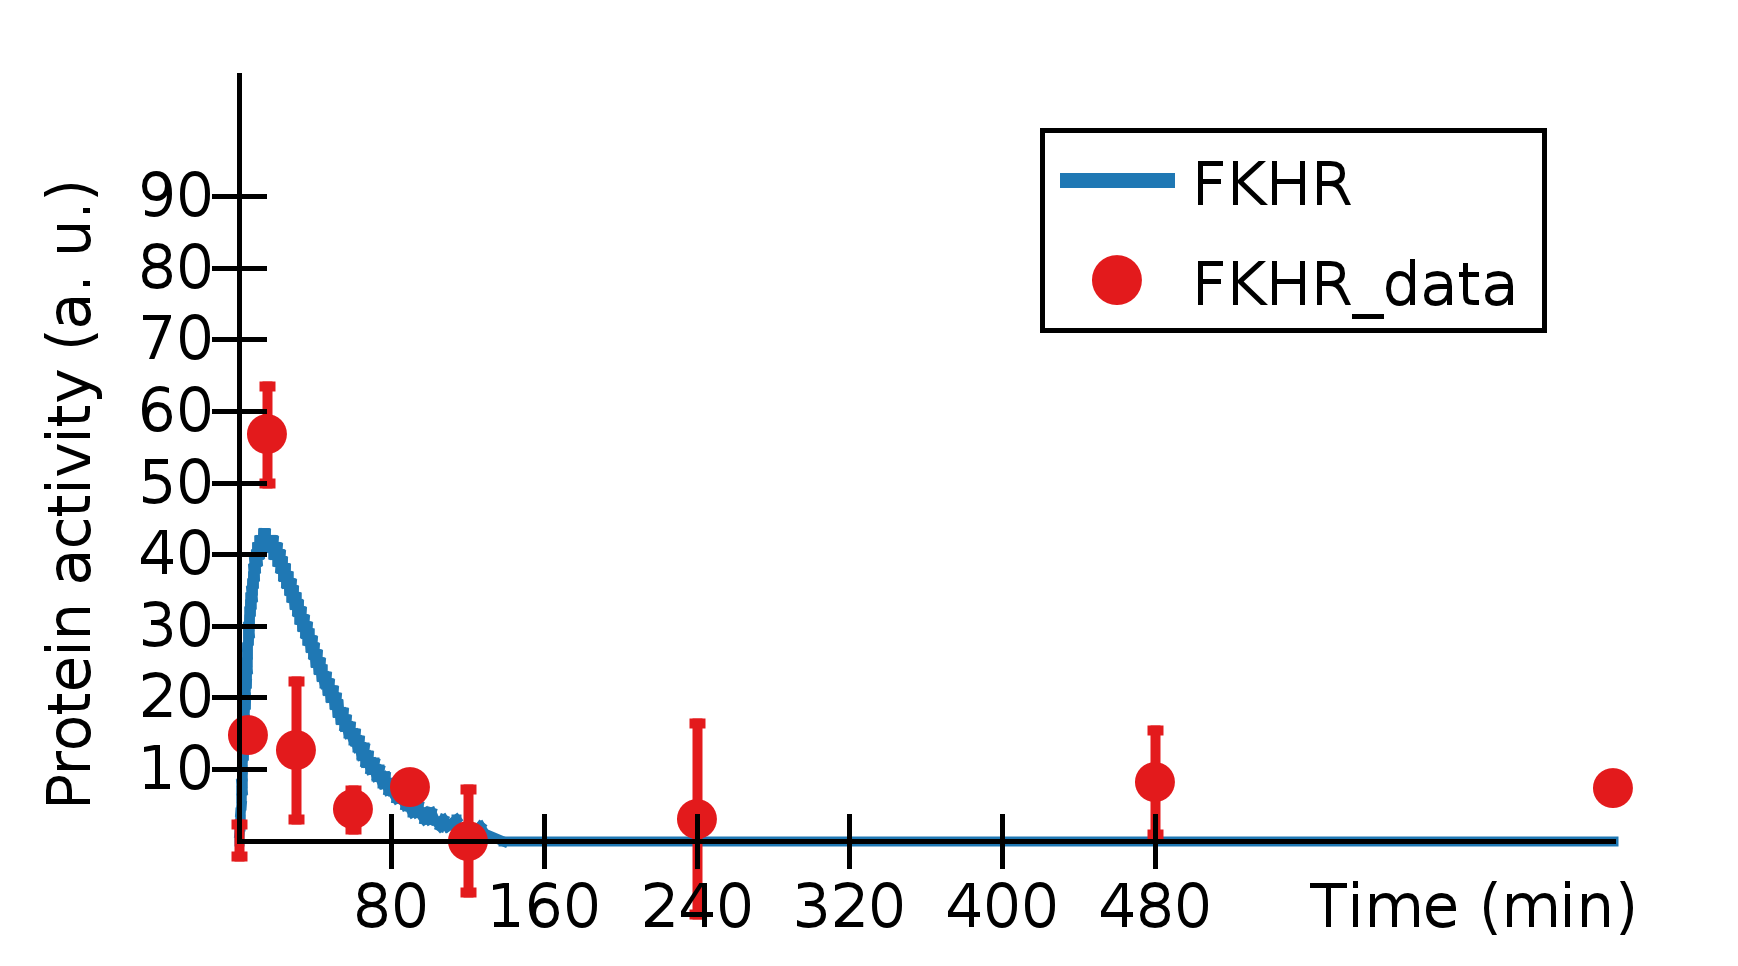
\includegraphics[width=0.29\textwidth]{images/EGF100/FKHR_720}}
\end{tabularx}
\caption{Comparison between the ANIMO model in Figure~\ref{fig:large-model-complete} and experimental data. Treatment condition: 100 ng/ml EGF.
In order to ease the comparison for earlier responses, the time span for those cases is less than 24 hours.}\label{fig:differences2}
\end{minipage}
\end{figure}


\begin{figure}[!tpb]
\begin{minipage}{\textwidth}
\begin{tabularx}{\textwidth}{XXX}
\subfloat[MK2 (2 hours)]{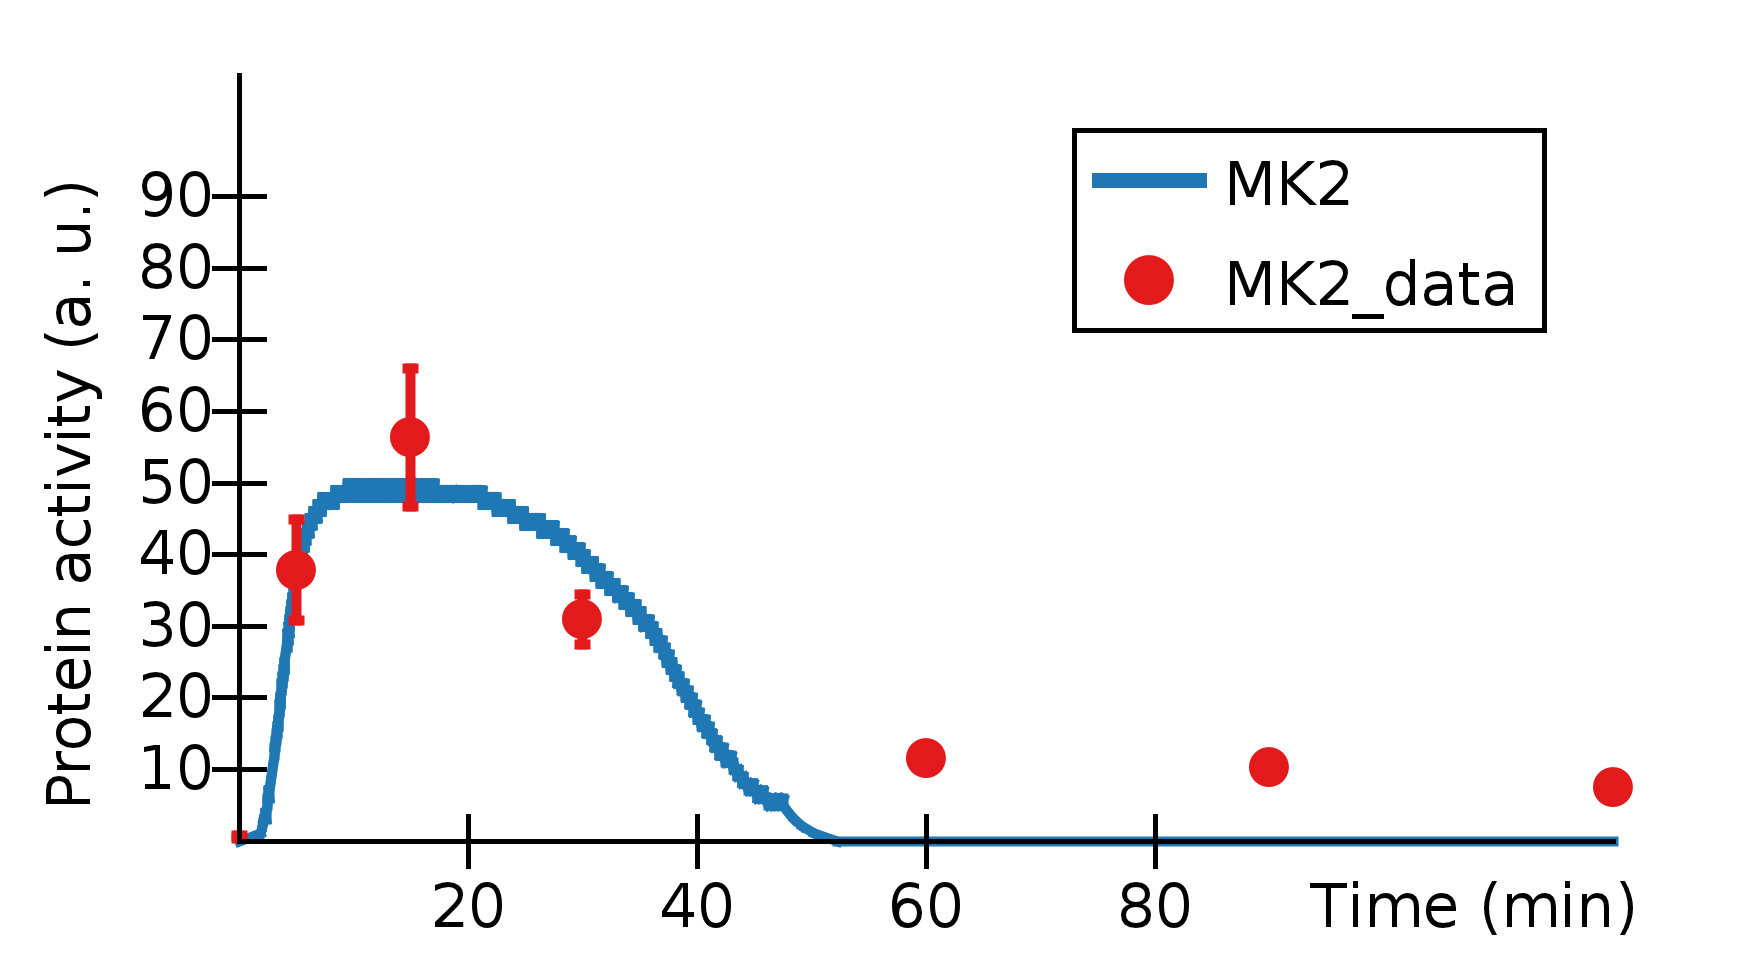
\includegraphics[width=0.29\textwidth]{images/TNFa100_EGF100/MK2}} &
\subfloat[JNK1 (2 hours)]{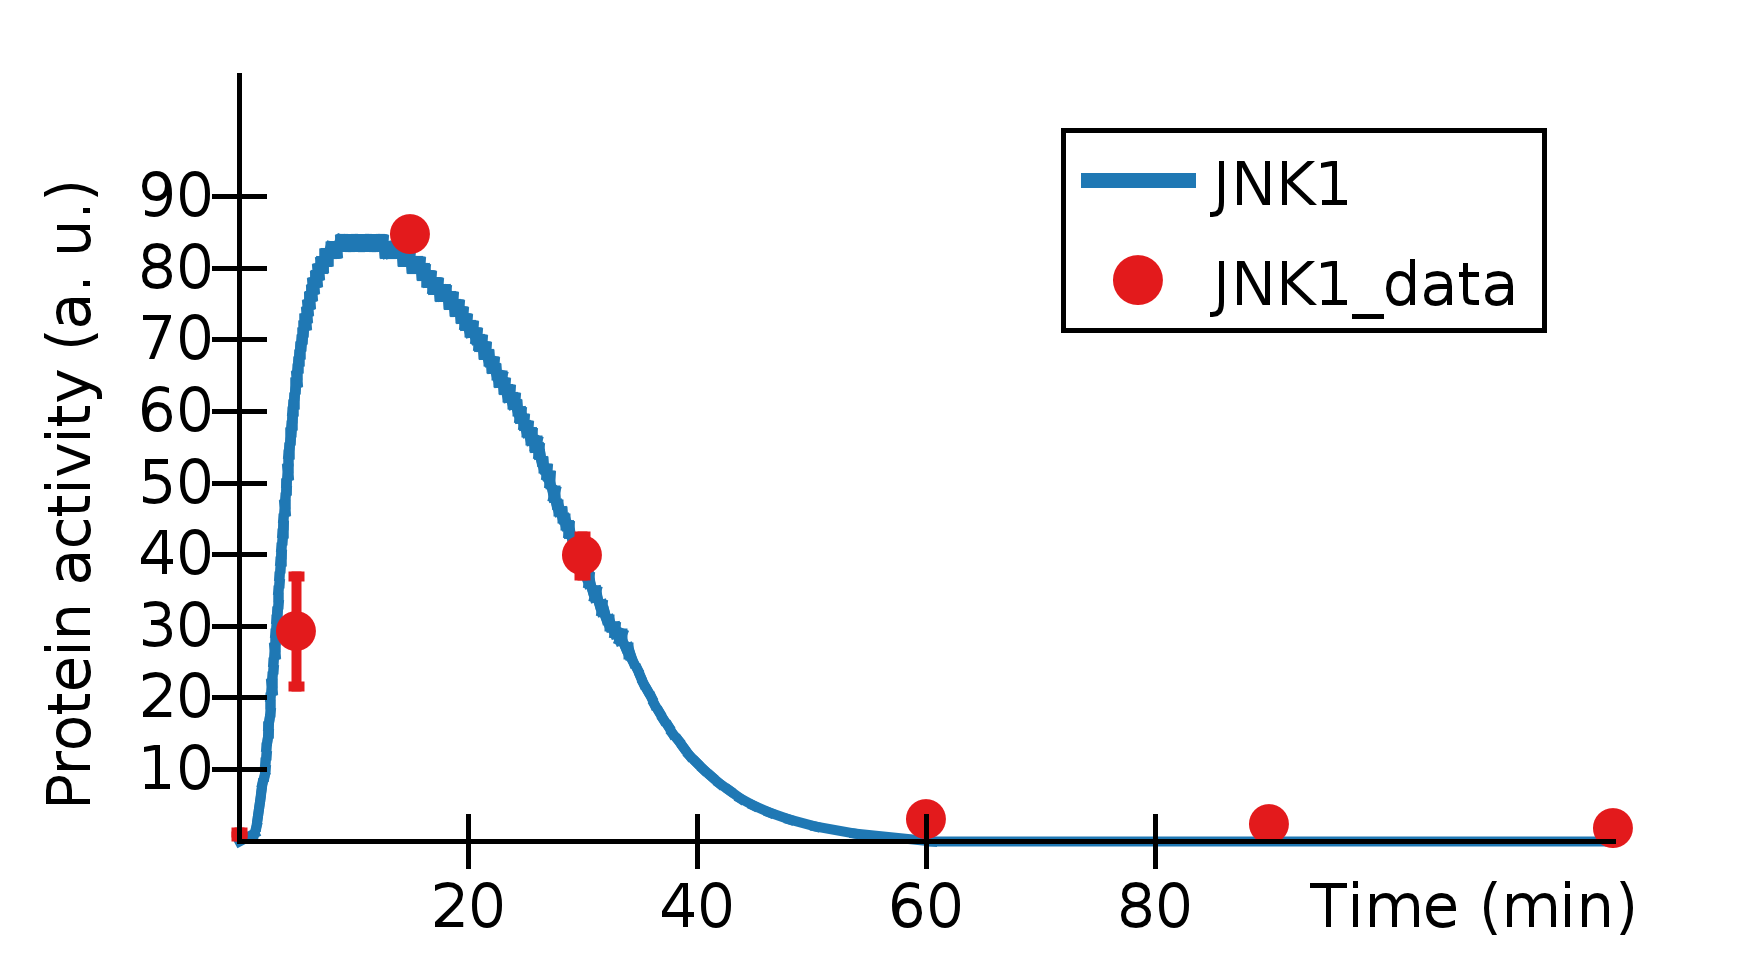
\includegraphics[width=0.29\textwidth]{images/TNFa100_EGF100/JNK1}} &
\subfloat[IKK (24 hours)]{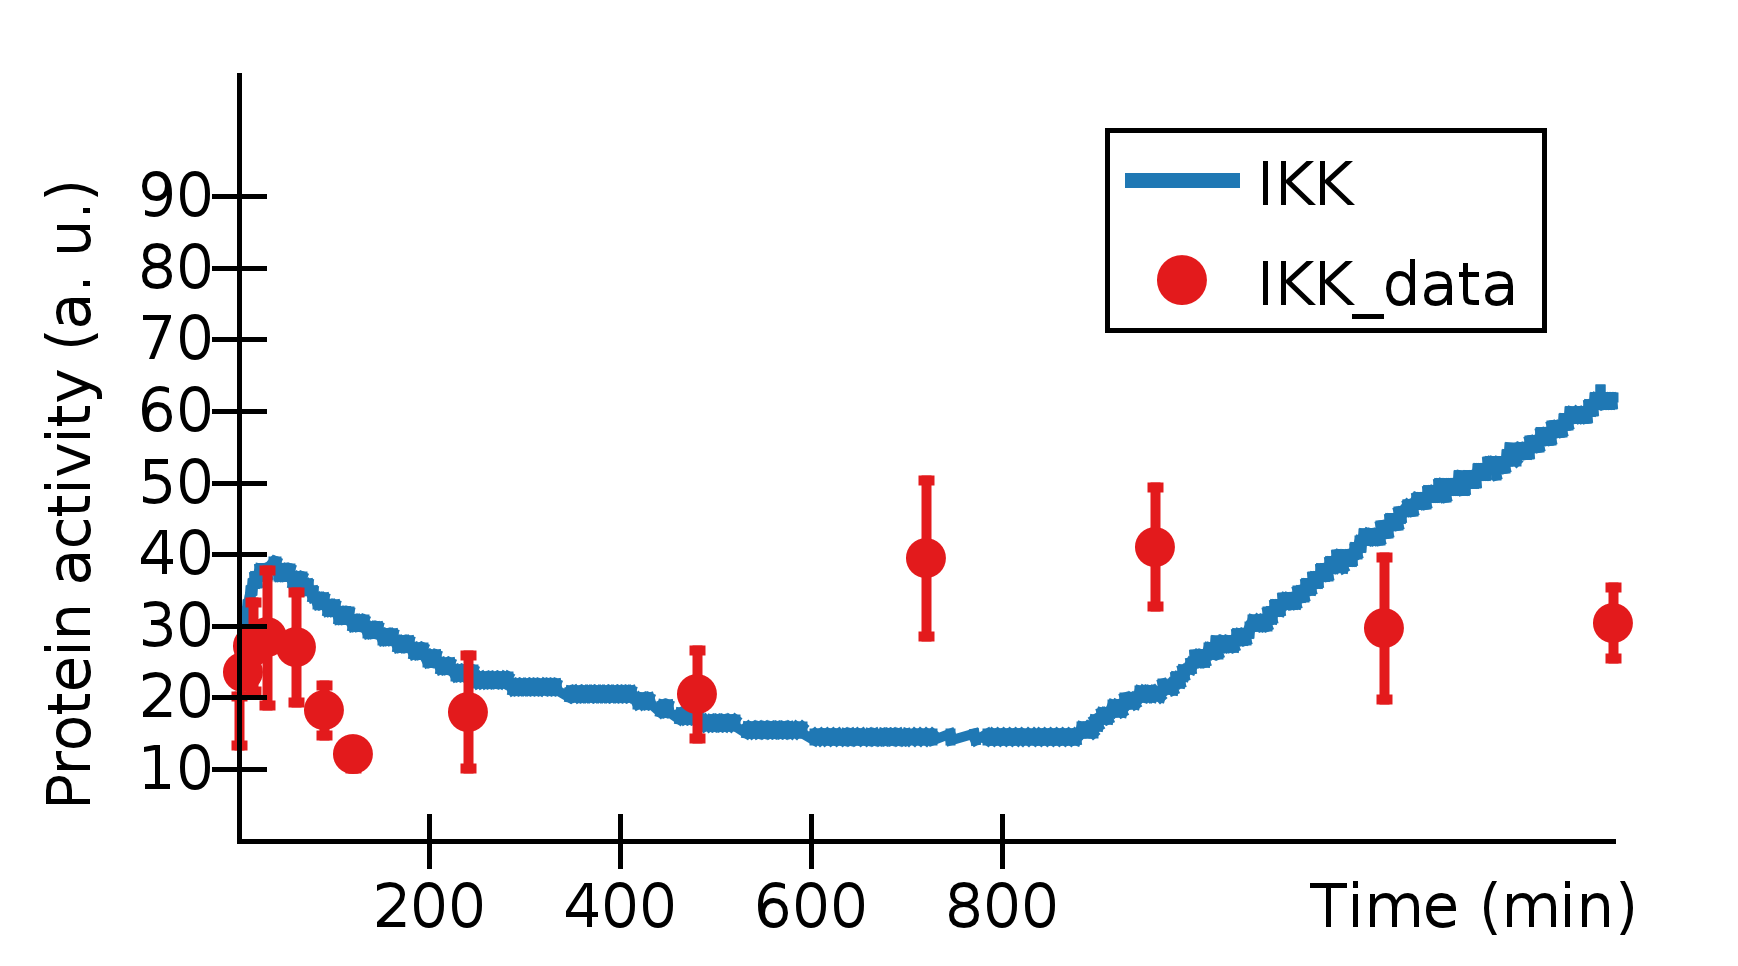
\includegraphics[width=0.29\textwidth]{images/TNFa100_EGF100/IKK}} \\
\subfloat[caspase-8 (24 hours)]{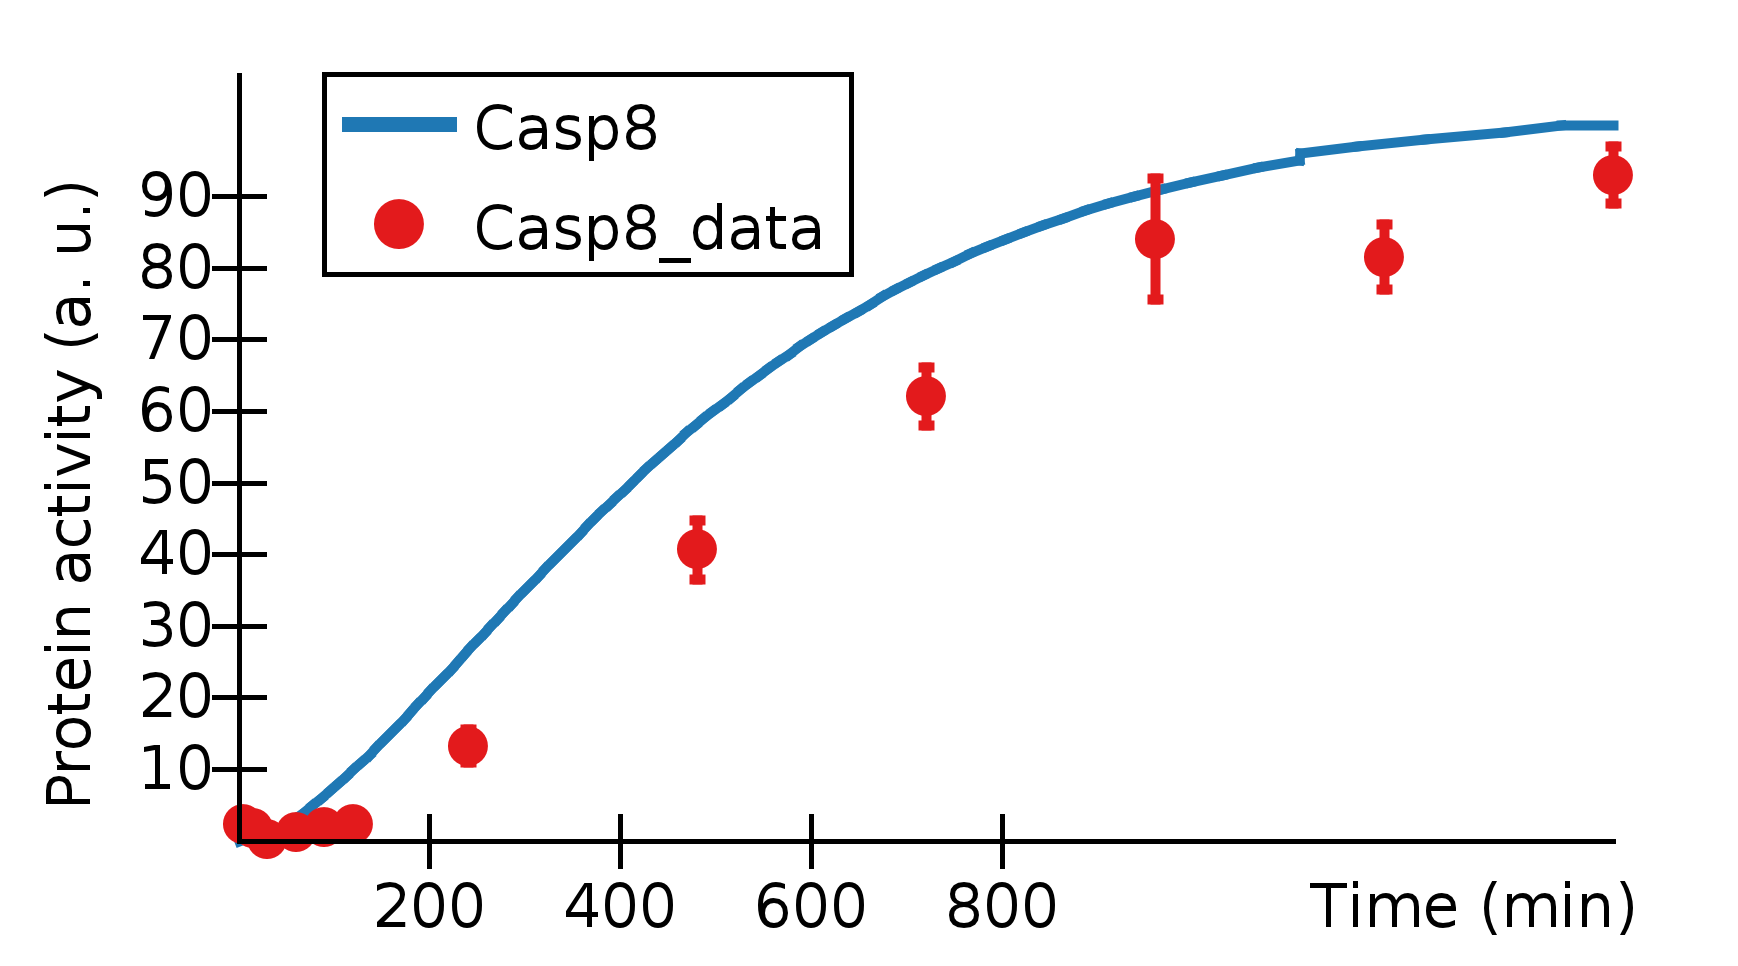
\includegraphics[width=0.29\textwidth]{images/TNFa100_EGF100/casp8}} &
\subfloat[caspase-3 (24 hours)]{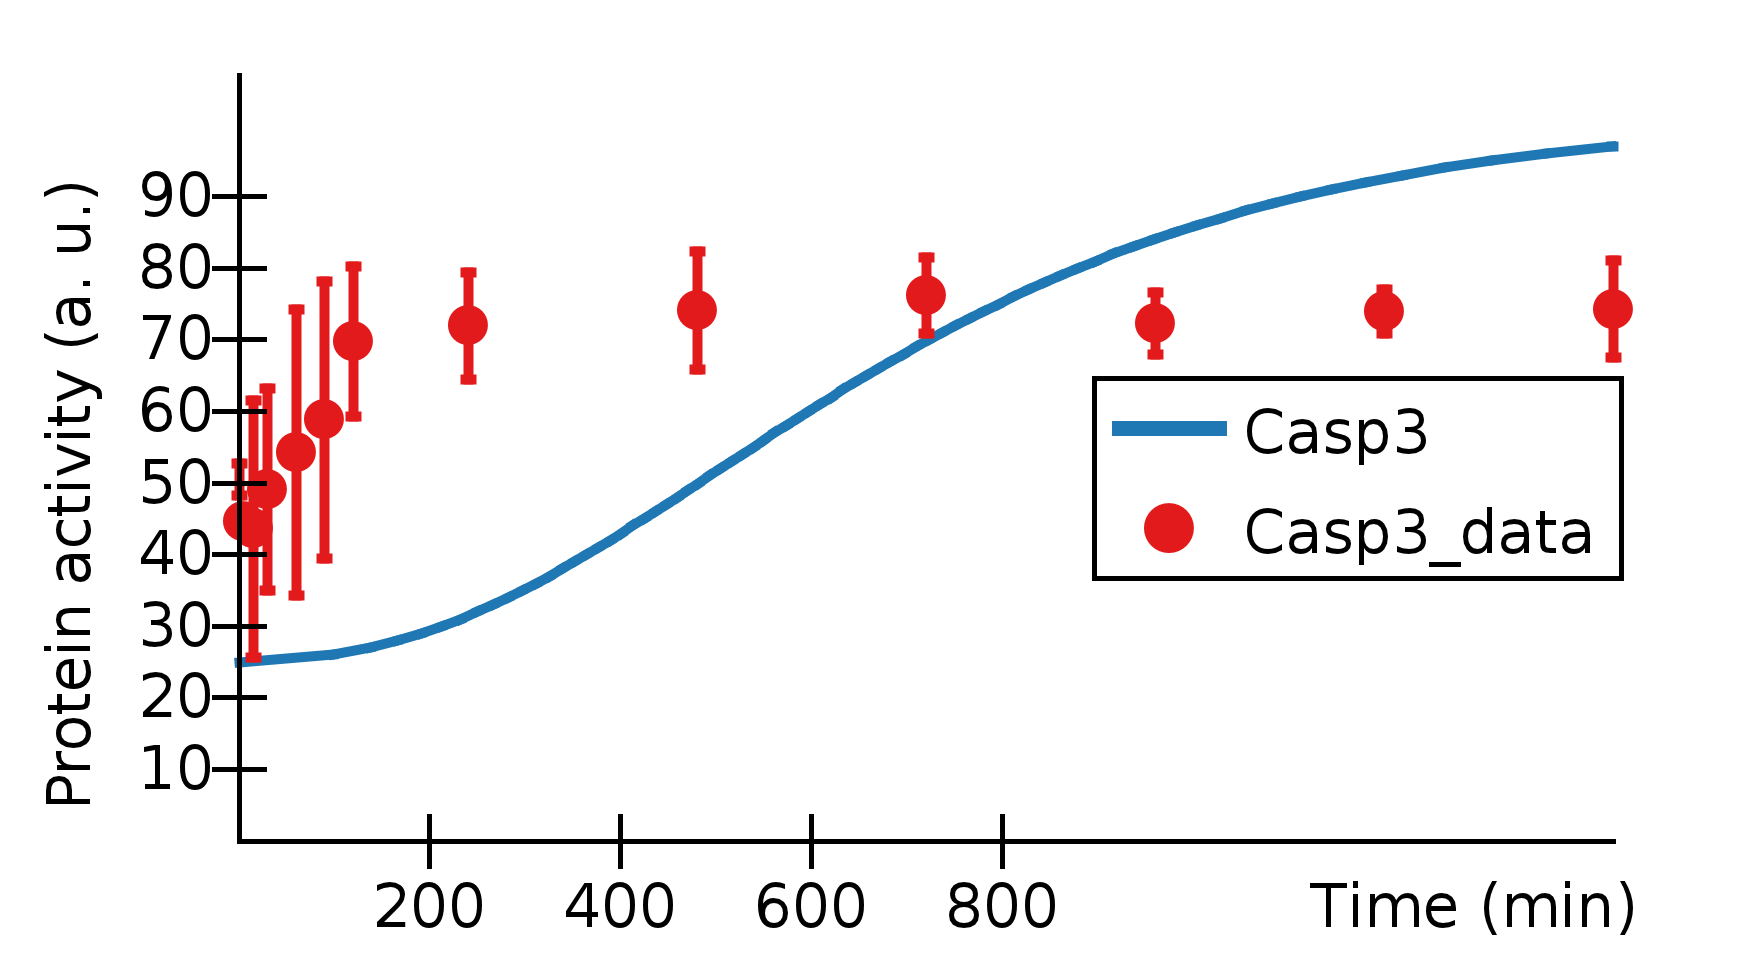
\includegraphics[width=0.29\textwidth]{images/TNFa100_EGF100/casp3}} &
\subfloat[MEK (2 hours)]{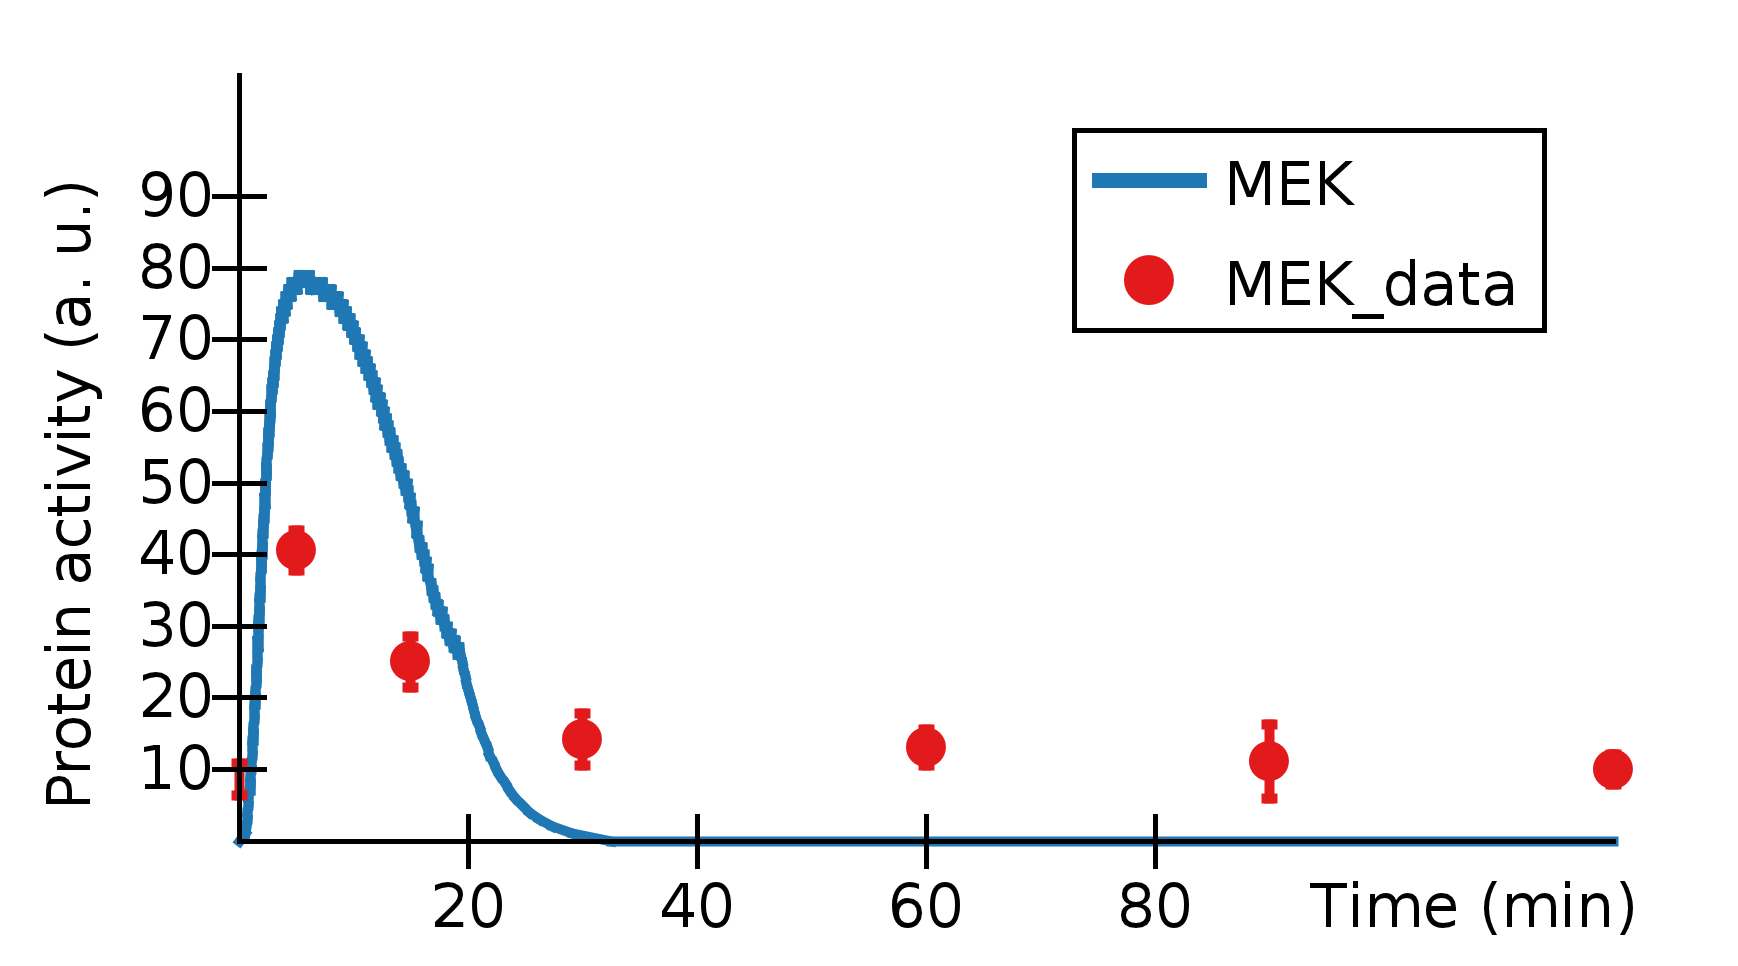
\includegraphics[width=0.29\textwidth]{images/TNFa100_EGF100/MEK}} \\
\subfloat[ERK (2 hours)]{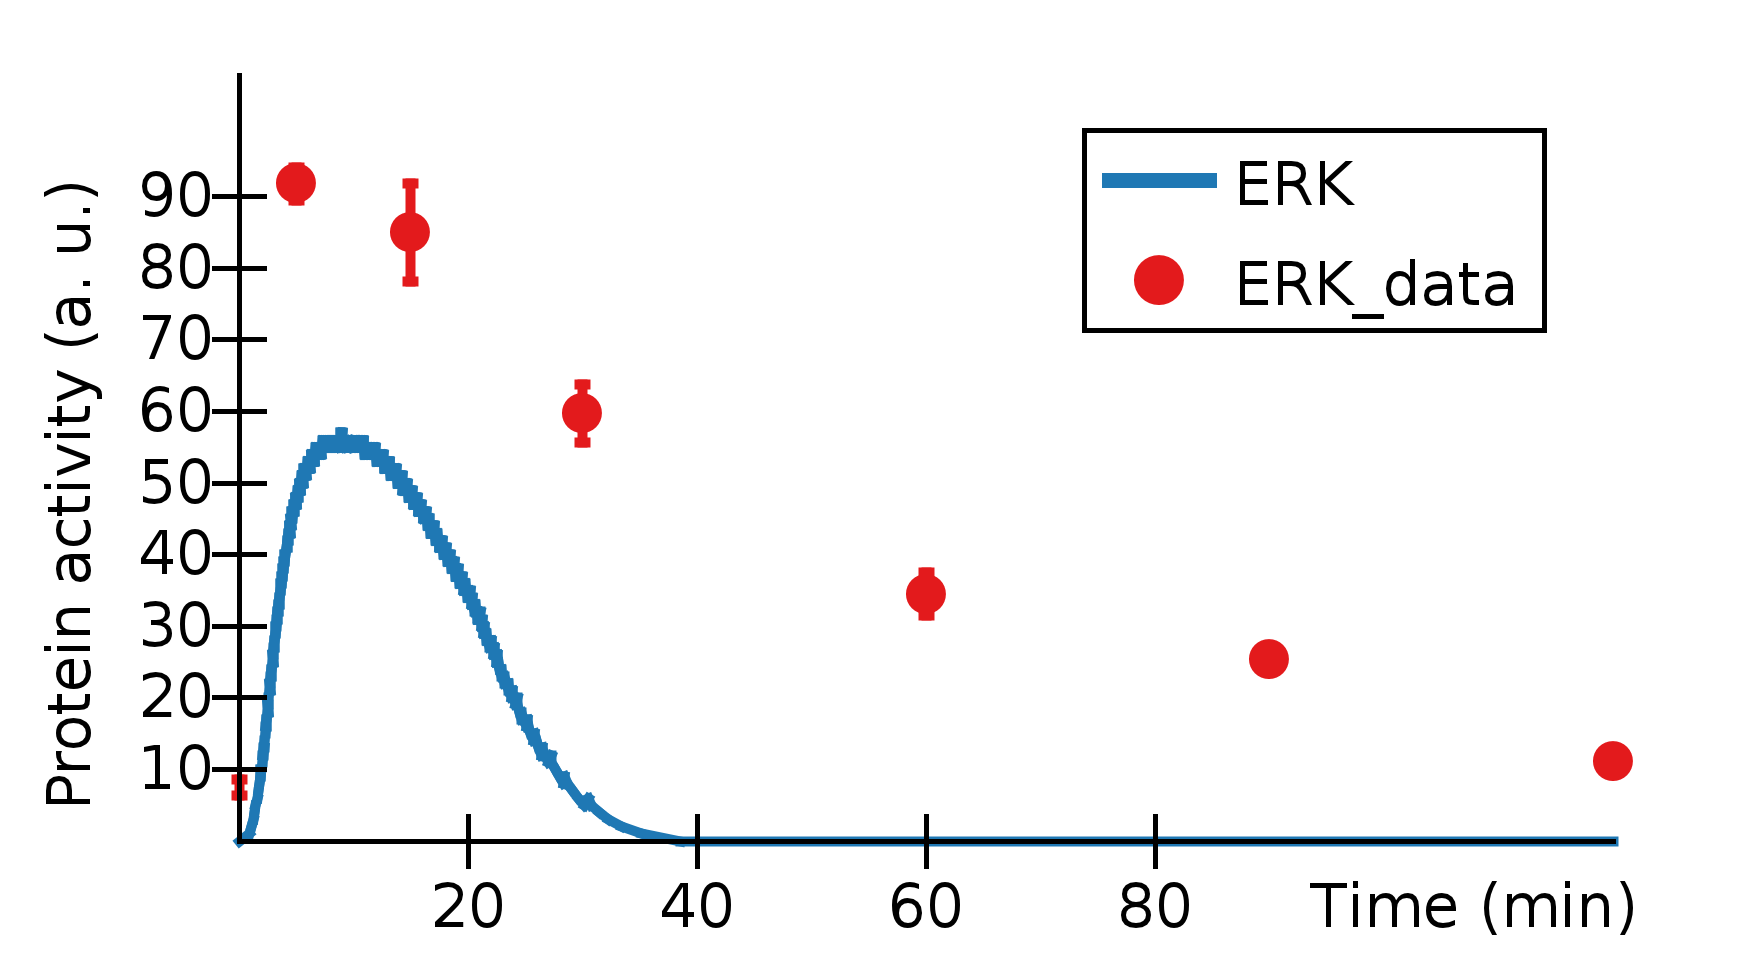
\includegraphics[width=0.29\textwidth]{images/TNFa100_EGF100/ERK}} &
\subfloat[Akt (2 hours)]{\includegraphics[width=0.29\textwidth]{images/TNFa100_EGF100/Akt}} &
\subfloat[IRS-1(S) (2 hours)]{\includegraphics[width=0.29\textwidth]{images/TNFa100_EGF100/IRS1s_120}} \\
\subfloat[IRS-1(S) (12 hours)]{\includegraphics[width=0.29\textwidth]{images/TNFa100_EGF100/IRS1s_720}} &
\subfloat[IRS-1(Y) (2 hours)]{\includegraphics[width=0.29\textwidth]{images/TNFa100_EGF100/IRS1y}} &
\subfloat[FKHR (4 hours)]{\includegraphics[width=0.29\textwidth]{images/TNFa100_EGF100/FKHR_240}}
\end{tabularx}
\caption{Comparison between the ANIMO model in Figure~\ref{fig:large-model-complete} and experimental data. Treatment condition: 100 ng/ml TNF$\alpha$ + 100 ng/ml EGF.
In order to ease the comparison for earlier responses, the time span for those cases is less than 24 hours.}\label{fig:differences3}
\end{minipage}
\end{figure}
